\pagebreak
%% ===========================================
\begin{tcolorbox}

\section{zzAdvice-on-Appendices}

\textbf{APPENDICES HOW TO Guidelines - TO REMOVE LATER}	
% \vspace*{1\baselineskip}

% ==========================================================
\lstset{basicstyle=\footnotesize, numberstyle=\tiny\color{blue}, frame=single, numbers=left, firstnumber=1, stepnumber=1, numbersep=1pt, xleftmargin=2.0em, framexleftmargin=1.5em, xrightmargin=0.0em, breaklines=true, breakatwhitespace=false, breakindent=5pt, prebreak=\space, postbreak=\space }
% ==========================================================
\begin{lstlisting}[caption={zzAdvice-on-Appendices}, label=zzAdvice-on-Appendices]

% (1) INFO FOR APPENDICES


% (2) PLACED INSIDE PREAMBLE SECTION

%% FOR APPENDIX FOR EACH CHAPTER
%% FOR DOCUMENT APPENDIX TESTED GOOD
	\usepackage{tocbibind}
	\usepackage[toc,page]{appendix}

% (3) PLACED INSIDE DOCUMENT SECTION

%% PLACED AT THE END JUST ABOVE INDEXING
%% FOR APPENDIX FOR EACH CHAPTER TEX FILE SEPARATELY
	\appendix
	\renewcommand{\thechapter}{\arabic{chapter}}
	\chapter{Appendices}
	\input{Chapter-8-Chapters-for-Appendices}

% (4) EXAMPLES

CONTENTS FOR Chapter-8-Chapters-for-Appendices TEX FILE
The contents of the appendices are organized according to chapters presented in the text. The appendices are as follows: 

\begin{enumerate}[start=1,label={(\bfseries \arabic*):}]
\item Chapter-1 Appendices (Introduction) [\ref{sec:App1-Introduction}] 
\item Chapter-2 Appendices (Literature Survey)[\ref{sec:App2-Literature-Survey}] 
\item Chapter-3 Appendices (Research Methodology)[\ref{sec:App3-Research-Methodology}] 
\item Chapter-4 Appendices (Related Research Work)[\ref{sec:App4-Related-Research-Work}] 
\item Chapter-5 Appendices (Research Implementation Plan)[\ref{sec:App5-Research-Implementation-Plan}] 
\end{enumerate}

\clearpage
\pagebreak
	
	%% SEPARATE FILES AS INPUT
	
	% ==========================================================
\clearpage
\pagebreak
\justifying
\renewcommand{\thesection}{A \arabic{section}}

\titleformat{\section}{\normalfont\LARGE\bfseries\color{black}}{\thesection}{10pt}{\LARGE}
\section{Appendix-A1 Introduction}\label{sec:App1-Introduction}

% ==========================================================	
\subsection{App1-CNC Milling Machine}
\begin{figure}[htbp]
	\begin{center}
		\frame{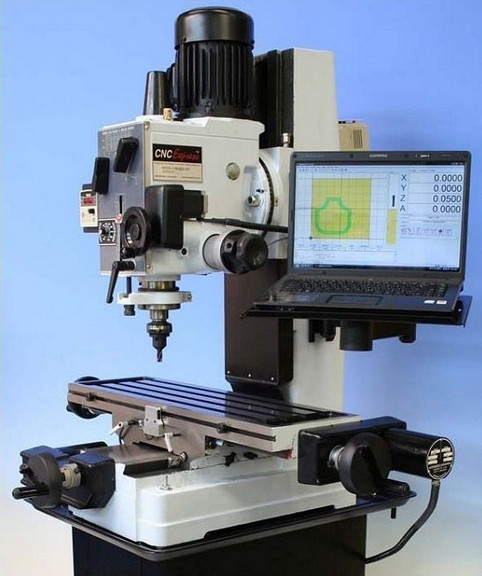
\includegraphics[width=0.5\textwidth]{./07-images/img-Ch1App/CNC-Milling-Machine.jpg}}
		\caption{App1-CNC Milling Machine}
		\label{fig:App1-CNC-Milling-Machine.jpg}
	\end{center}
\end{figure}

% ==========================================================
\subsection{App1-CNC Lathe Machine}
\begin{figure}[htbp]
	\begin{center}
		\frame{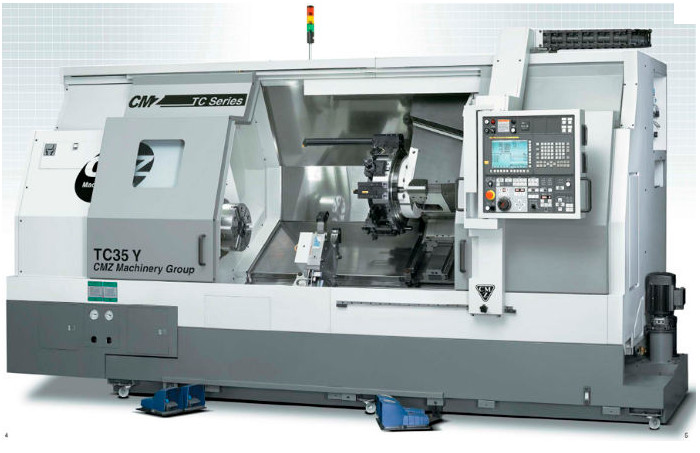
\includegraphics[width=0.5\textwidth]{./07-images/img-Ch1App/CNC-Lathe-Machine.jpg}}
		\caption{App1-CNC Lathe Machine}
		\label{fig:App1-CNC-Lathe-Machine.jpg}
	\end{center}
\end{figure}

% ==========================================================
\clearpage
\pagebreak
\subsection{App1-CNC Routing Machine}
\begin{figure}[htbp]
	\begin{center}
		\frame{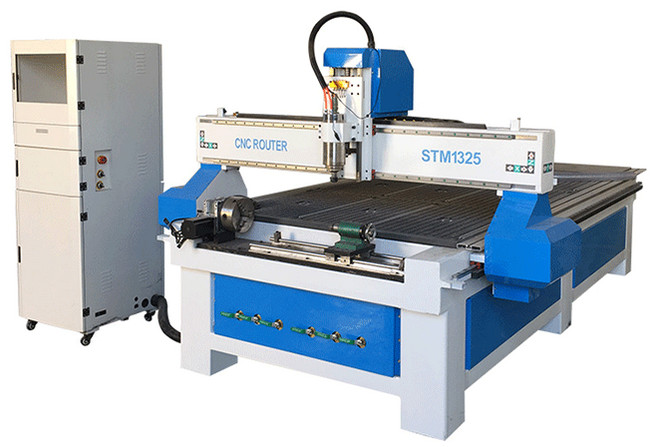
\includegraphics[width=0.50\textwidth]{./07-images/img-Ch1App/CNC-Routing-Machine.jpg}}
		\caption{App1-CNC Routing Machine}
		\label{fig:App1-CNC-Routing-Machine.jpg}
	\end{center}
\end{figure}

% ===========================================================
\subsection{App1-CNC 3D Printing Machine}
\begin{figure}[htbp]
	\begin{center}
		\frame{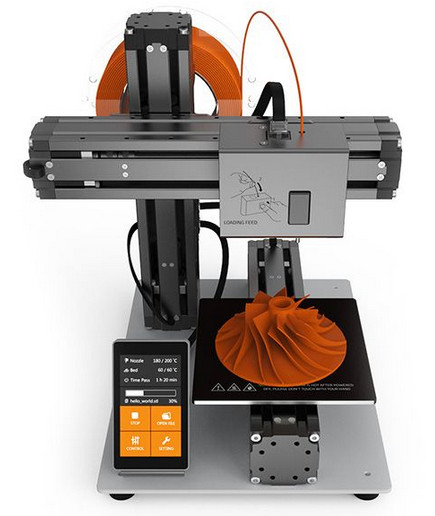
\includegraphics[width=0.5\textwidth]{./07-images/img-Ch1App/CNC-3D-Printing-Machine.jpg}}
		\caption{App1-CNC 3D Printing Machine}
		\label{fig:App1-CNC-3D-Printing-Machine.jpg}
	\end{center}
\end{figure}

% ==========================================================
 %% Introduction
	% ==========================================================
\clearpage
\pagebreak
\justifying
\renewcommand{\thesection}{B \arabic{section}}

\titleformat{\section}{\normalfont\LARGE\bfseries\color{black}}{\thesection}{10pt}{\LARGE}
\section{Appendix-B2 Literature Survey}\label{sec:App2-Literature-Survey}

% ==========================================================
\clearpage
\begin{landscape}
\subsection{App2-Ha Scilab NURBS versus Octave NURBS}
	
	\begin{table}[ht]
		\begin{center}
			\caption{App2-Scilab NURBS versus Octave NURBS}		
			\label{table:App2-Scilab NURBS versus Octave NURBS}	
			
			\begin{tabular}{ |p{0.5cm}|p{5.0cm}|p{9.0cm}|p{9.0cm}|}
				\rowcolor{gray!10}			
				\hline \multicolumn{4}{|c|}{\textbf{Scilab NURBS versus Octave NURBS}} \\ [1.0ex]
				\rowcolor{gray!10}
				\hline \textbf{No} & \textbf{Specifications}    & \textbf{Hewlett Packard EliteBook 8470p} & \textbf{Hewlett Packard ProBook 440G}\\ 
				
				\hline 1 & Name of Student    & Wan Ruslan bin W Yusoff & hello\\ 
				\hline 2 & Student ID         &  aaa & Hello\\ 
				\hline 3 & National Reg. ID   & bbb  & Hello\\ 
				\hline 4 & Faculty            & ccc  & Hello\\ 
				
				\hline
			\end{tabular}
		\end{center}
	\end{table}  
	
	
\end{landscape}
% ==========================================================
% ==========================================================
\clearpage
\begin{landscape}
	\subsection{App2-Scilab NURBS versus Octave NURBS}
	
	\begin{table}[ht]
		\begin{center}
			\caption{App2-Computer Notebook Specifications}		
			\label{tabl2:App2-Computer Notebook Specifications}	
			
			\begin{tabular}{ |p{0.5cm}|p{5.0cm}|p{9.0cm}|p{9.0cm}|}
				\rowcolor{gray!10}			
				\hline \multicolumn{4}{|c|}{\textbf{Computer Notebook Specifications}} \\ [1.0ex]
				\rowcolor{gray!10}
				\hline \textbf{No} & \textbf{Specifications}    & \textbf{Hewlett Packard EliteBook 8470p} & \textbf{Hewlett Packard ProBook 440G}\\ 
				
				\hline 1 & Name of Student    & Wan Ruslan bin W Yusoff & hello\\ 
				\hline 2 & Student ID         &  aaa & Hello\\ 
				\hline 3 & National Reg. ID   & bbb  & Hello\\ 
				\hline 4 & Faculty            & ccc  & Hello\\ 
				
				\hline
			\end{tabular}
		\end{center}
	\end{table}  
	
	
\end{landscape}
% ==========================================================
% ==========================================================

\clearpage
\begin{landscape}
	\subsection{App2-Bla bla bla}
	
	\begin{table}[ht]
		\begin{center}
			\caption{App2-Computer Notebook Specifications}		
			\label{table:App2-Computer Notebook Specifications}	
			
			\begin{tabular}{ |p{0.5cm}|p{5.0cm}|p{9.0cm}|p{9.0cm}|}
				\rowcolor{gray!10}			
				\hline \multicolumn{4}{|c|}{\textbf{Computer Notebook Specifications}} \\ [1.0ex]
				\rowcolor{gray!10}
				\hline \textbf{No} & \textbf{Specifications}    & \textbf{Hewlett Packard EliteBook 8470p} & \textbf{Hewlett Packard ProBook 440G}\\ 
				
				\hline 1 & Name of Student    & Wan Ruslan bin W Yusoff & hello\\ 
				\hline 2 & Student ID         &  aaa & Hello\\ 
				\hline 3 & National Reg. ID   & bbb  & Hello\\ 
				\hline 4 & Faculty            & ccc  & Hello\\ 
				
				\hline
			\end{tabular}
		\end{center}
	\end{table}  
	
	
\end{landscape}
% ==========================================================
% ========================================================== %% Literature Survey
	% ==========================================================
\clearpage
\pagebreak
\justifying
\renewcommand{\thesection}{C \arabic{section}}

\titleformat{\section}{\normalfont\LARGE\bfseries\color{black}}{\thesection}{10pt}{\LARGE}
\section{Appendix-C3 Research Methodology}\label{sec:App3-Research-Methodology}

% ==========================================================
\subsection{App3-Pico Universal PWM Servo Controller}\label{sec:C-3.1-Universal PWM Servo Controller Board}
				
\begin{figure}[htbp]
	\begin{center}
		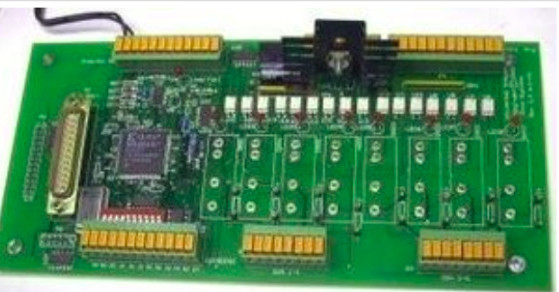
\includegraphics[width=0.85\textwidth]{./07-images/img-Ch3App/Universal-PWM-Servo-Controller.jpg}
		\caption{App3-Universal PWM Servo Controller Parallel Port Interface Board}
		\label{fig:App3-Universal-PWM-Servo-Controller.jpg}
	\end{center}
\end{figure}

\subsection{App3-Specifications Pico Universal PWM Servo Controller}

Reference: \url{http://www.pico-systems.com/motion.html}
\vspace{0.5cm}

The Universal PWM Servo Controller is a small board with everything needed to control a 2-axis, 3-axis or 4-axis machine tool with PWM-driven servo amplifiers. It contains 4 PWM generators with variable PWM drive frequency, 4 digital encoder counters to follow the machine position, 16 channels of opto-isolated digital inputs, and 8 positions for Solid State Relays of your choice to be mounted. It is connected to a computer by the parallel port. The parallel port must be at least capable of bi-directional exchange of data, but EPP or ECP modes give the best data transfer rate. The digital I/O section also implements emergency stop logic. There is an on board watchdog timer, which can be set to cause an emergency stop in case the computer fails to update the PWM generators in a timely fashion. This could shut off the servo amps, spindle motor, coolant, etc. For machines with more than 4 axes, 2 or more boards can be used together.
\vspace{0.5cm}

The computer reads the position from the encoder counters and computes a new PWM duty cycle to send to the PWM generators. This takes only about 50 uS on a 333 MHz Pentium II, so that reasonable servo update rates of 10 KHz could be made on such a machine. I usually use 1 KHz, because that is all that seems needed for machine-tool type applications.
\vspace{0.5cm}

The PWM generators divide a 10 MHz crystal clock by a minimum of 2 up to 216-1, which comes out to 5 MHz down to 153 Hz. A PWM frequency of 1 to 100 KHz is practical, and can be selected to suit the servo amplifiers. The duty cycle of the PWM waveform can be programmed in 100 nS steps, which is 1 percent at 100 KHz, but 0.2 percent at 20 KHz. The PWM and direction outputs can source or sink 12 mA to drive opto-coupled amplifier inputs.
\vspace{0.5cm}

The encoder counters keep a continuous watch over the encoder signals and can count up to 300,000 encoder counts/second, per channel. (The rev 5.x and later boards have an adjustable digital filter so that counting above 5 MHz can be performed.) They can also sense the index pulse from an encoder which has this feature. This can be used to more precisely locate the home position. If the encoder has no index channel, connect the index input (Z) to A.
\vspace{0.5cm}

The digital input section has 16 opto-isolators which can sense the condition of switches, relays, pressure switches, float sensors, etc. to allow the machine to be stopped if a fault condition occurs, sense when an axis is close to the travel limit or home position, etc. The board provides isolated 5V power to power the switches and/or sensors.
\vspace{0.5cm}

The digital output section provides sockets for up to 8 Opto-22 compatible Solid State Relays to be mounted directly onto the board. These sites are left unpopulated to allow the user to select SSRs with the output configuration and current capacity needed. A terminal strip is provided for connection to the outputs of the SSRs. LEDs monitor the command signal to each of the SSRs.
\vspace{0.5cm}

The last digital input is configured to monitor an emergency stop chain. A series circuit of normally-closed switches breaks the continuity of the circuit when an unsafe condition or problem develops (ie. spindle motor stall, servo amp overheat, lube level low, manual E-stop switch activated, etc.) An analog timer circuit can also monitor the flow of commands from the computer, and if the computer ceases updating the rate generators, then an E-stop can be caused. The E-stop condition turns off all signals to the solid state relays, as well as stopping the PWM generators, to bring the machine to a safe stop.
\vspace{0.5cm}

This boards contains a power regulator that produces all power needed by it from a provided 'wall-wart' type plug-in power supply.
\vspace{0.5cm}

The Universal PWM Controller takes advantage of the IEEE-1284 hardware signalling protocol, allowing multiple register addresses to be selected and transfers accomplished with minimum CPU overhead, and maximum data transfer rate. This requires a parallel port that can operate in the ECP or EPP mode. A male-female DB-25 cable specifically designed for IEEE-1284 compatability is required. Note: You MUST use a cable marked "IEEE-1284 compliant" for this system to work reliably.

% ==========================================================
\pagebreak
\subsection{App3-MCU Microchip 28-Pin LIN Development Board}\label{sec:C-3.3-MCU Microchip 28-Pin LIN Development Board}
				
\begin{figure}[htbp]
	\begin{center}
		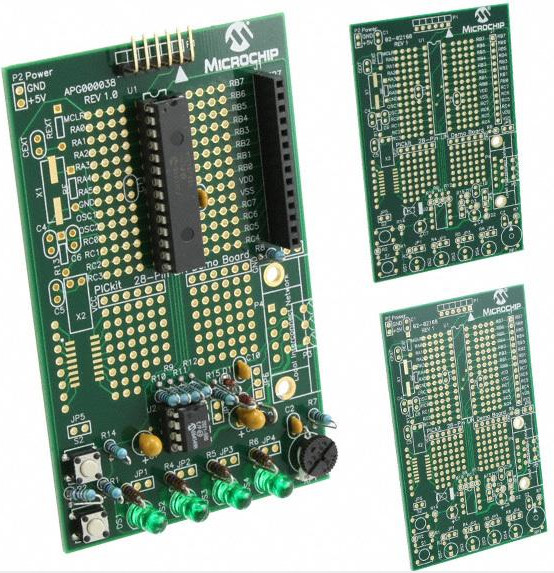
\includegraphics[width=0.95\textwidth]{./07-images/img-Ch3App/MCU-Microchip-Dev-Demo-Board.jpg}
		\caption{App3-MCU Microchip 28-Pin LIN Development Demo Interface Board}
		\label{fig:App3-MCU-Microchip-Dev-Demo-Board.jpg}
	\end{center}
\end{figure}

\subsection{App3-Specifications MCU Microchip 28-Pin LIN Development Board}

Reference: \url{https://www.digikey.my/products/en?keywords=DM164130-3-ND\%20\%20}\\
28-Pin LIN DEMO BOARD USER'S GUIDE\\
2009 Microchip Technology Inc.DSxxxxx\\
\vspace{0.5cm}

The 28-Pin LIN (Local Interconnect Network) Demo Board is a small and simple demonstration PCB for Microchip's 28-pin Dual Inline Package (DIP) PIC Microcontroller Units (MCU). It is populated with a PIC16F886 MCU, a MCP2021 LIN Transceiver with voltage regulator, four LEDs, 2 push buttons and a potentiometer. The demo board has several test points to access the I/O pins of the MCU and a generous prototyping area. The MCU can be programmed with the PICkit 2 Microcontroller Programmer or the MPLAB ICD 2 using the RJ-11 to 6-pin inline adapter (AC164110).
\vspace{0.5cm}

LIN (Local Interconnect Network) is an automotive networking technology, a sub-bus system based on a serial communications protocol. The bus is a single master/multiple slave bus that uses a single wire to transmit data.
\vspace{0.5cm}

The 28-Pin LIN Demo Board can be used with virtually any 28-pin Dual Inline Package (DIP) PIC MCU. The assembled 28-Pin LIN Demo Board is populated with a PIC16F886-I/P microcontroller. Additional 28-Pin LIN Demo Boards can be ordered from Microchip technology and distributors. Part number, DM164120-3, comes with one assembled and two blank 28-Pin LIN Demo Boards. 
\vspace{0.5cm}

The blank demo board can be used for evaluating or prototyping circuits using any of the 28-pin devices listed below.

\begin{figure}[htbp]
	\begin{center}
		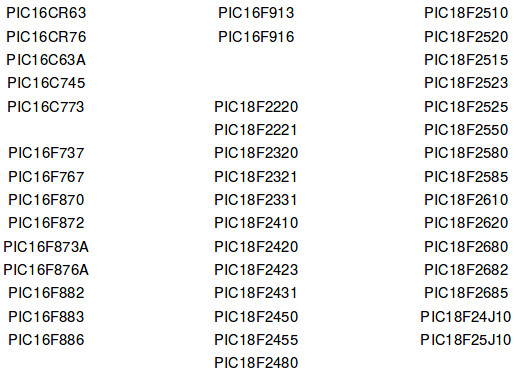
\includegraphics[width=0.85\textwidth]{./07-images/img-Ch3App/MCU-Chips-Supported-for-Dev-Demo-Board.jpg}
		\caption{App3-MCU Chips Supported-for Dev Demo Interface Board}
		\label{fig:App3-MCU-Chips-Supported-for-Dev-Demo-Board.jpg}
	\end{center}
\end{figure}

The 28-Pin LIN Demo Board is populated with a PIC16F886 MCU (U1), a MCP2021 LIN Transceiver with Voltage Regulator (U2), four LEDs (DS1-DS4), Two push buttons (SW1 and SW2), 32 KHz crystal (X2) and potentiometer (RP1). The board layout is shown in the figure below. The demo board has several test points to access the I/O pins of the MCU and a generous prototyping area. The MCU can be programmed with the PICkit 2 Microcontroller Programmer from header P1.
\vspace{0.5cm}

\pagebreak
\begin{figure}[htbp]
	\begin{center}
		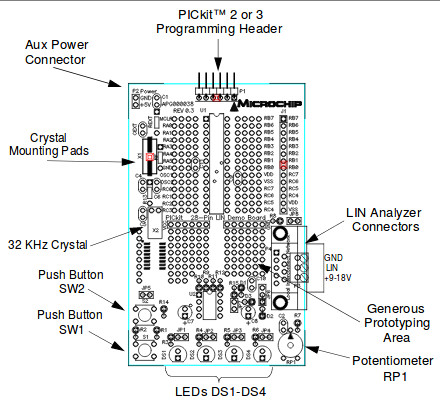
\includegraphics[width=0.95\textwidth]{./07-images/img-Ch3App/MCU-Microchip-28-Pin-LIN-Dev-Demo-Board.jpg}
		\caption{App3-MCU Microchip 28-Pin LIN Dev Demo Board Layout Diagram}
		\label{fig:App3-MCU-Microchip-28-Pin-LIN-Dev-Demo-Board.jpg}
	\end{center}
\end{figure}



% ==========================================================
\pagebreak
\subsection{App3-MCU Microchip Curiosity Development Board}\label{sec:C-3.5-Curiosity-Development-Board}

\begin{figure}[htbp]
	\begin{center}
		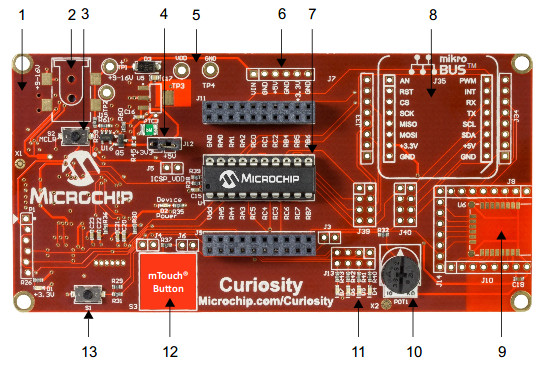
\includegraphics[width=0.85\textwidth]{./07-images/img-Ch3App/MCU-Curiosity-Dev-Board-Layout.jpg}
		\caption{App3-MCU Microchip Curiosity Demo Board Layout Diagram}
		\label{fig:App3-MCU-Curiosity-Dev-Board-Layout.jpg}
	\end{center}
\end{figure}
\begin{figure}[htbp]
	\begin{center}
		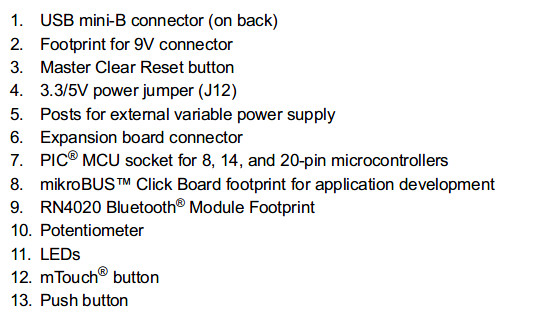
\includegraphics[width=0.65\textwidth]{./07-images/img-Ch3App/MCU-Curiosity-Dev-Board-Layout-Legend.jpg}
		\caption{App3-MCU Microchip Curiosity Demo Board Layout Legend}
		\label{fig:App3-MCU-Curiosity-Dev-Board-Layout-Legend.jpg}
	\end{center}
\end{figure}

\pagebreak
\subsection{App3-Specifications MCU Microchip Curiosity Development Board}
Reference: Curiosity Development Board User's Guide\\
2015-2016 Microchip Technology Inc. DS40001804B\\
\vspace{0.5cm}

The Curiosity Development Board supports Microchip's 8-pin, 14-pin and 20-pin 8-bit PIC MCUs. Dual-row expansion headers on either side of the socket offer flexibility of connectivity to all pins on the PIC MCUs. This board provides flexibility for 
experimentation through an application header with ground (GND) and supply voltage (VDD) connections. It also includes
a set of indication LEDs, mTouch button and push-button switches, and a variable potentiometer. Additionally, it features a 
Bluetooth low-energy footprint and a mikroBUS footprint to accommodate a variety of plug-in Click Board sensors that can be used in application development.
\vspace{0.5cm}

The Curiosity Development Board can be powered in one of three ways, depending on its usage.
\vspace{0.5cm}

\textbf{Power1 via USB Connector (J2)}\\

The USB connector (J2) will power the entire Curiosity Development Board. A shunt jumper must be placed onto jumper J12. The right two pins of J12 will connect +5V from the USB connector J2. The left two pins of J12 will connect +3.3V from the USB voltage regulator on the back side of the development board. With USB power connected to J2, power LED D1 will always be ON to indicate that +3.3V is available on the board. 
\vspace{0.5cm}

\textbf{Power2 via 9V External Power Supply (J15)}\\
%\vspace{0.5cm}

The 9V external power supply (J15) will also power the entire Curiosity Development Board. A shunt jumper must be placed onto jumper J12. The right two pins of J12 will connect +5V from the on-board voltage regulator circuitry connected to connector J15. The left two pins of J12 will connect +3.3V from the on-board voltage regulator circuitry. With 9V external power connected to J15, power LED D1 will always be ON to indicate that +3.3V is available on the board. Power LED D2 will only be ON when power (+3.3V or +5V) is applied to VDD via a shunt jumper placed on J12.
\vspace{0.5cm}

\textbf{Power3 via Variable External Power Supply (TP3, TP4)}\\
%\vspace{0.5cm}

A variable external power supply connected to TP3 and TP4 will power the entire Curiosity Development Board. A shunt jumper is not needed on J12, thus either +3.3V or +5V can be directly applied via a variable external power supply to VDD.
\vspace{0.5cm}


\textbf{Getting Started on Curiosity Board}\\
%\vspace{0.5cm}

The Curiosity Development Board must be used with MPLAB X Integrated Development Environment (IDE), available free on Microchip's web site, www.microchip.com. Use version v3.05 or later. The Curiosity Development Board, through MPLAB X, is a low-voltage in-circuit debugger, as well as a low-voltage programmer, for all supported devices. In-circuit debugging allows the user to run, examine and modify programs for the supported device embedded in the Curiosity hardware. This facilitates
the debugging of firmware and hardware concurrently. Use the Curiosity Development Board with MPLAB X IDE to run, stop and single-step through programs breakpoints can be set and the processor can be reset. When the processor stops, the contents of the register are available for examination and modification.
\vspace{0.5cm}

\textbf{Programming the Curiosity Board}\\
%\vspace{0.5cm}

After connecting the Curiosity Development Board to the computer using the on-board USB connector (J2 on the back of the board), open the MPLAB X IDE. Then create a new project or open an existing project. Click on the Project Properties icon located in the project's Dashboard window.
\vspace{0.5cm}

Alternatively, the Project Properties window can be opened by clicking on File, Project Properties, or by right-clicking on 
the project name in the Projects window and clicking Properties.
\vspace{0.5cm}

And it goes on.

% ==========================================================
 %% Research Methodology
	% ==========================================================
\clearpage
\pagebreak
\justifying
\renewcommand{\thesection}{D \arabic{section}}

\titleformat{\section}{\normalfont\LARGE\bfseries\color{black}}{\thesection}{10pt}{\LARGE}
\section{Appendix-D4 Related Research Work}\label{sec:App4-Related-Research-Work}

%% PORTRAIT
%\pagebreak
%\clearpage
% ==========================================================
\clearpage
\pagebreak
\section{Some Results on Previous Projects}

Bismillah



%% PORTRAIT
\pagebreak
\clearpage
% ==========================================================
\clearpage
\pagebreak
%% \section{Images of Devices for Previous Projects}

\subsection{App4-Parallel Port Devices}. 
				
		\begin{figure}[htbp]
			\begin{center}
				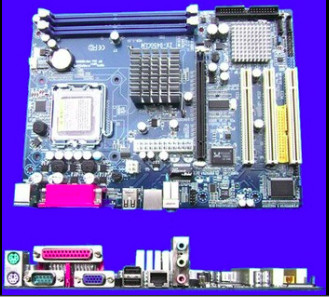
\includegraphics[width=0.700\textwidth]{./07-images/img-Ch4/Captured-Parallel-Port-Built-in-Motherboard.jpg}
				\caption{App4-Parallel Port device built-in on Motherboard (purple)}
				\label{fig:App4-Captured-Parallel-Port-Built-in-Motherboard.jpg}
			\end{center}
		 \end{figure}
		 
		
		\begin{figure}[htbp]
			\begin{center}
\frame{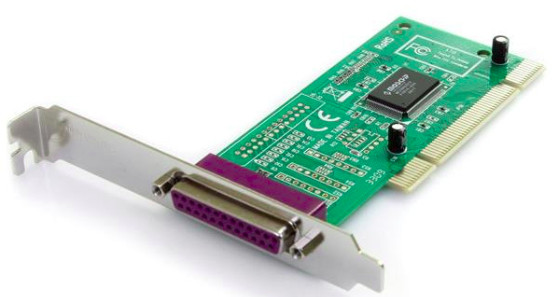
\includegraphics[width=0.65\textwidth]{./07-images/img-Ch4/Captured-Parallel-Port-PCI-Adapter-Card.jpg}}
				\caption{App4-Parallel Port PCI Adapter Card}
				\label{fig:App4-Captured-Parallel-Port-PCI-Adapter-Card.jpg}
			\end{center}
		\end{figure}
The Netmos Nm9805 is a IEEE 1284 parallel port controller with PCI bus interface. Nm9805 fully supports the existing Centronics printer interface as well as PS/2, EPP, and ECP modes. Single 5V operation. Low power. PCI compatible 1284 printer port. Multi-mode compatible controller (SPP, PS2, EPP, ECP). Fast data rates up to 1.5 Mbytes/s (parallel port). Microsoft and Linux compatible. 

% ==================
\clearpage
\pagebreak
		\begin{figure}[htbp]
			\begin{center}
\frame{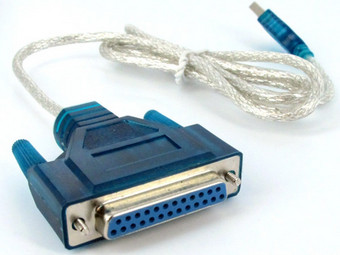
\includegraphics[width=0.65\textwidth]{./07-images/img-Ch4/Captured-USB-to-Parallel-Port-PL2305-Converter.jpg}}
				\caption{App4-USB to Parallel Port PL2305 Converter Cable}
				\label{fig:App4-Captured-USB-to-Parallel-Port-PL2305-Converter.jpg}
			\end{center}
		\end{figure}

		\begin{figure}[htbp]
			\begin{center}
\frame{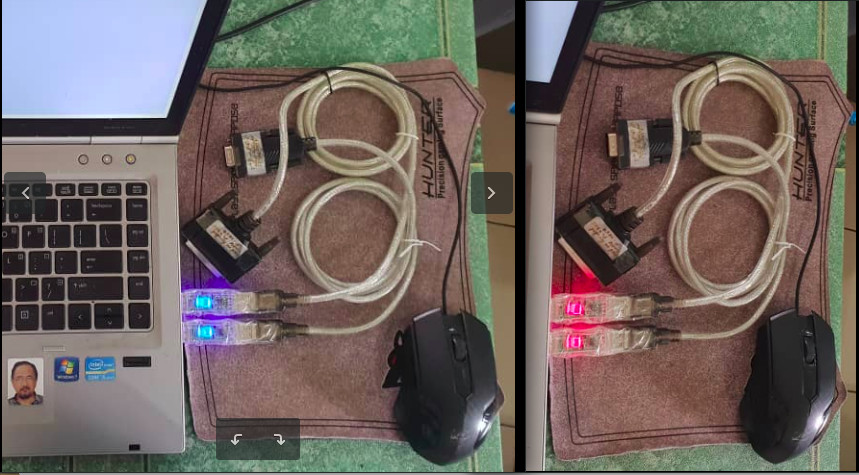
\includegraphics[width=0.75\textwidth]{./07-images/img-Ch4/USB-to-Serial-Parallel-Idle-and-Writing-Modes.jpg}}
				\caption{App4-USB to-Serial and to-Parallel Idle(Left) and Writing(Right) Modes}
				\label{fig:App4-USB-to-Serial-Parallel-Idle-and Writing-Modes.jpg}
			\end{center}
		\end{figure}
		
LEFT PICTURE: The blue color LED status is for cable device idle and ready.\\
RIGHT PICTURE: The red color LED status is for cable device busy during active reading and writing modes.  
	
\lstset{basicstyle=\ttfamily\small}
%% \lstset{basicstyle=\ttfamily\tiny}
\begin{lstlisting}[breaklines, frame=single, caption={App4-Detection of USB-to-Parallel Cable}, label=App4-usb-to-paralle-PL2305-cable-detected]
Bus 001 Device 021: ID 067b:2305 Prolific Technology, Inc. 
PL2305 Parallel Port  <=== FOUND 
[ 3978.848284] usb 1-1.6: Manufacturer: Prolific Technology Inc.
[ 3978.855271] usblp 1-1.6:1.0: usblp0: USB Bidirectional 
printer dev 21 if 0 alt 1 proto 2 vid 0x067B pid 0x2305
\end{lstlisting}

		
% ==================
\clearpage
\pagebreak
		
\subsection{App4-Velleman K8000 Parallel Interface Board}

	\begin{figure}[htbp]
		\begin{center}
\frame{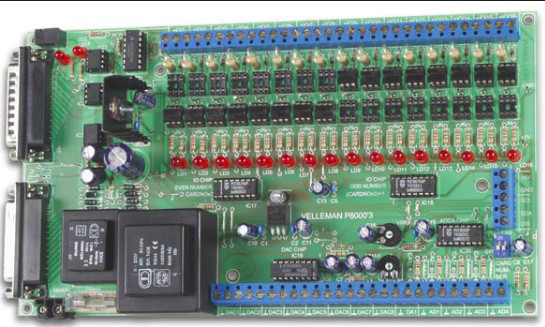
\includegraphics[width=0.85\textwidth]{./07-images/img-Ch4/Captured-Velleman-K8000-Parallel-Port-Extension-Board.jpg}}
			\caption{App4-Velleman K8000 Parallel Port Extension Board}
			\label{fig:App4-Captured-Velleman-K8000 Parallel-Port-Extension-Board.jpg}
		\end{center}
	\end{figure}
	
\lstset{basicstyle=\ttfamily\small}
%% \lstset{basicstyle=\ttfamily\tiny}
\begin{lstlisting}[breaklines, frame=single, caption={App4-Specifications of Velleman K8000 Parallel Interface Board}, label=App4-Specifications-Velleman-K8000-Interface-Board]
DIGITAL OUTPUTS:
    optocoupler, open collector output: 50mA - max. 30VDC
DIGITAL INPUTS:
    optocoupler input: 5V/5mA, max. 20V/40mA
ANALOG OUTPUTS:
    8 outputs DAC1 to DAC8, resolution: 64 steps
    minimum output voltage: 0.1V at 2mA
    maximum output voltage: 11.5V adjustable at 2mA
    resolution per step from 0.1 to 11.5V: 160mV +/- 90mV
    1 precision output DA1, resolution: 256 steps
    minimum output voltage: 0V
    maximum output voltage: 4.5V adjustable at 0.5mA
    resolution per step from 0 to 4.5V: 17.5mV
ANALOG INPUTS:
    4 analogue inputs AD1 to AD4, resolution: 256 steps
    minimum input voltage: 0V
    maximum input voltage: 5V
    input impedance: 50Mohm
    resolution: 19.5mV
    communication protocol: I2Cbus
    LED indication for each I/O
BOARD:
    25 pin D series connector for computer
    25 pin D series connector for printer
    supply voltage: 230Vac
    PCB dimensions: 237 x 133mm (9.3" x 5.2")
\end{lstlisting}			
			
%================================================		
\clearpage
\pagebreak		
		
\subsection{App4-Velleman K8055 USB Interface Board}
	
\begin{figure}[htbp]
	\begin{center}
\frame{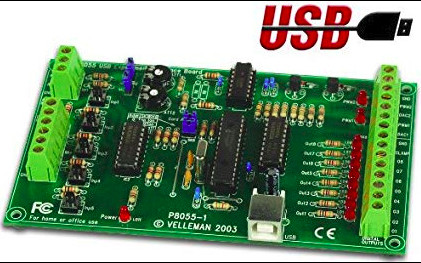
\includegraphics[width=0.85\textwidth]{./07-images/img-Ch4/Captured-Velleman-K8055-USB-Extension-Board.jpg}}
\caption{App4-Velleman K8055 USB Port Extension Board}
\label{fig:App4-Captured-Velleman-K8055-USB-Extension-Board.jpg}
	\end{center}
\end{figure}

\lstset{basicstyle=\ttfamily\small}
%% \lstset{basicstyle=\ttfamily\tiny}
\begin{lstlisting}[breaklines, frame=single, caption={App4-Specifications of Velleman K8055 USB Interface Board}, label=App4-Specifications-Velleman-K8055-USB-Interface-Board]
DIGITAL INPUTS:
    5 digital inputs (0 = ground, 1 = open) 
    (on board test buttons provided)
ANALOG INPUTS:
    2 analogue inputs with attenuation and amplification 
    option (internal test +5V provided)
DIGITAL OUTPUTS:
    8 digital open collector output switches 
    (max. 50V/100mA) (on board LED indication)
ANALOG OUTPUTS:
    2 analogue outputs:
    0 to 5V, output resistance 1K5
    PWM 0 to 100% open collector outputs 
    max 100mA / 40V (on board LED indication)
    general conversion time: 20ms per command
BOARD:    
    power supply through USB: approx. 70mA
    dimensions: 145 x 88 x 20mm / 5.7 x 3 x 0.8"
\end{lstlisting}


%================================================		
\clearpage
\pagebreak

\subsection{App4-Heber X10i USB Board}.

\begin{figure}[htbp]
	\begin{center}
		\frame{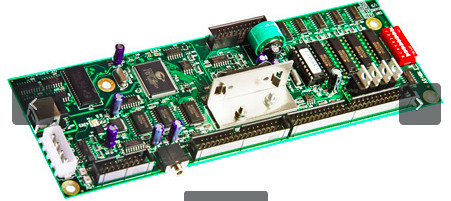
\includegraphics[width=0.85\textwidth]{./07-images/img-Ch4/Captured-Heber-X10i-USB-Extension-Board.jpg}}
		\caption{App4-Heber X10i USB Port Extension Board}
		\label{fig:App4-Captured-Heber-X10i-USB-Extension-Board.jpg}
	\end{center}
\end{figure}


\lstset{basicstyle=\ttfamily\small}
%% \lstset{basicstyle=\ttfamily\tiny}
\begin{lstlisting}[breaklines, frame=single, caption={App4-Specifications of Heber-X10i USB Interface Board}, label=App4-Specifications-Heber-X10i-USB-Interface-Board]
Heber X10i = USB real-time PC I/O controller
HARDWARE:
	64 Switched Inputs / Outputs
	Real-time I/O processor
	Battery backed SRAM
	Secure data retention
	DALLAS unique identifier
	Audio amp 5W RMS, Stereo audio amplifier
	Serial I/O
	SEC meter
	ccTalk
	LED control
	EEPROM 32KB
	Real time clock
	Current sensing 12v supply
	Open drain outputs for lamps and meters
	High current outputs
SOFTWARE:
	Serial I/O: RS232, TTL, ccTalk
	On-board security device
	Program in C, C+, C# or BlitzMax
	Microsoft Windows XPe / Linux / Raspberry Pi drivers
\end{lstlisting}

%================================================		
\clearpage
\pagebreak		
		
\subsection{App4-Arduino Due USB Board}. 

\begin{figure}[htbp]
	\begin{center}
		\frame{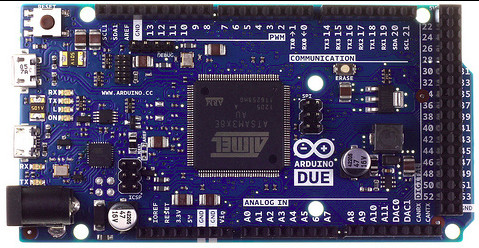
\includegraphics[width=0.85\textwidth]{./07-images/img-Ch4/Captured-Arduino-Due-USB-Extension-Board.jpg}}
		\caption{App4-Arduino Due USB Port Extension Board}
		\label{fig:App4-Captured-Arduino-Due-USB-Extension-Board.jpg}
	\end{center}
\end{figure}

Unlike most Arduino boards, the Arduino Due board runs at 3.3V. The maximum voltage that the I/O pins can tolerate is 3.3V. Applying voltages higher than 3.3V to any I/O pin could damage the board. 
\vspace*{1\baselineskip}

The SAM3X provides one hardware UART and three hardware USARTs for TTL (3.3V) serial communication.

\lstset{basicstyle=\ttfamily\small}
%% \lstset{basicstyle=\ttfamily\tiny}
\begin{lstlisting}[breaklines, frame=single, caption={App4-Specifications of Arduino Due USB Interface Board}, label=App4-Specifications-Arduino-Due-USB-Interface-Board]
Microcontroller 	AT91SAM3X8E
Operating Voltage 	3.3V
Input Voltage (recommended) 7-12V
Input Voltage (limits) 	6-16V
Digital I/O Pins 	54 (of which 12 provide PWM output)
Analog Input Pins 	12
Analog Output Pins 	2 (DAC)
Total DC Output Current on all I/O lines 	130 mA
DC Current for 3.3V Pin 	800 mA
DC Current for 5V Pin 	800 mA
Flash Memory 	512 KB all available for the user applications
SRAM 	96 KB (two banks: 64KB and 32KB)
Clock Speed 	84 MHz
Length 	101.52 mm
Width 	53.3 mm
Weight 	36 g
\end{lstlisting}

%================================================		
\clearpage
\pagebreak
		
\subsection{App4-Nexys-3 Spartan-6 FPGA USB Board}. 


\begin{figure}[htbp]
	\begin{center}
\frame{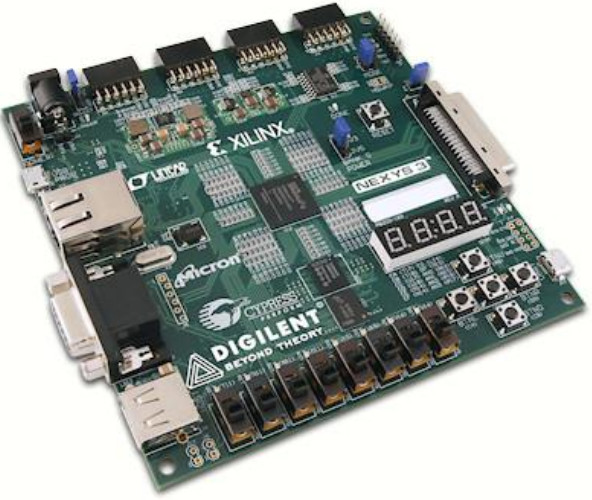
\includegraphics[width=0.80\textwidth]{./07-images/img-Ch4/Captured-Nexys3-Spartan6-FPGA-USB-Extension-Board.jpg}}
		\caption{App4-Nexys-3 Spartan-6 FPGA USB Port Extension Board}
		\label{fig:App4-Captured-Nexys3-Spartan6-FPGA-USB-Extension-Board.jpg}
	\end{center}
\end{figure}

Nexys 3 is compatible with all Xilinx CAD tools, including ChipScope, EDK, and the free WebPack. The Nexys 3 uses Digilent's newest Adept USB2 system that offers FPGA and ROM programming, automated board tests, virtual I/O, and simplified user data transfer facilities. In our project we used the Adept USB2 system.

\lstset{basicstyle=\ttfamily\small}
%% \lstset{basicstyle=\ttfamily\tiny}
\begin{lstlisting}[breaklines, frame=single, caption={App4-Specifications of Nexys-3 Spartan-6 FPGA USB Interface Board}, label=App4-Specifications-Nexys-3-Spartan-6-FPGA-USB-Interface-Board]
Xilinx Spartan-6 LX16 FPGA in a 324 pin BGA package
16 Mbyte Cellular RAM (x16)
16Mbytes SPI (quad mode) PCM non volatile memory
16Mbytes parallel PCM non volatile memory
10/100 Ethernet PHY
On board USB2 port for programming and data xfer
USB UART and USB
HID port (for mouse/keyboard)
8 bit VGA port
100 MHz CMOS oscillator
72 I/Os routed to expansion connectors
GPIO includes 8 LEDs, 5 buttons, 8 slide switches and 
4-digit seven segment display
USB v2 - programming cable included
\end{lstlisting}


%================================================		
\clearpage
\pagebreak

\subsection{App4-Raspberry Pi-3 Model-B Single Board Computer}. 

\begin{figure}[htbp]
	\begin{center}
		\frame{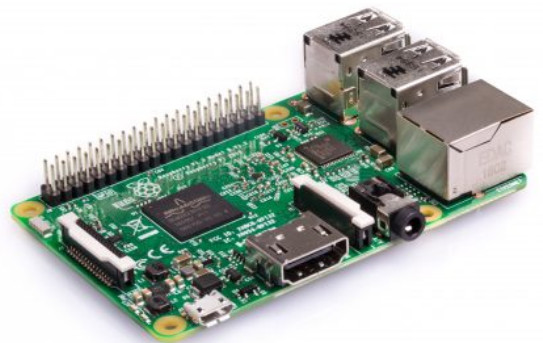
\includegraphics[width=0.85\textwidth]{./07-images/img-Ch4/Captured-Raspberry-Pi3-ModelB-SBC.jpg}}
		\caption{App4-Raspberry Pi-3 Model-B Single Board Computer}
		\label{fig:App4-Captured-Raspberry-Pi3-ModelB-SBC.jpg}
	\end{center}
\end{figure}

\subsection{App4-Raspberry Pi-2 Model-B Single Board Computer}.

\begin{figure}[htbp]
	\begin{center}
		\frame{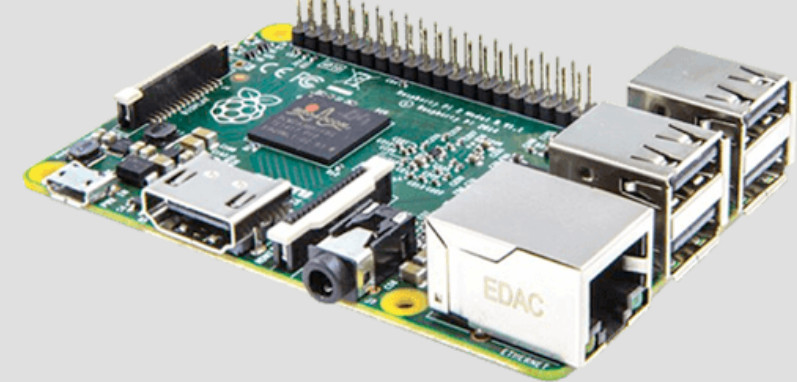
\includegraphics[width=0.85\textwidth]{./07-images/img-Ch4/Captured-Raspberry-Pi2-ModelB-SBC.jpg}}
		\caption{App4-Raspberry Pi-2 Model-B Single Board Computer}
		\label{fig:App4-Captured-Raspberry-Pi2-ModelB-SBC.jpg}
	\end{center}
\end{figure}

%================================================		
\clearpage
\pagebreak

\lstset{basicstyle=\ttfamily\small}
%% \lstset{basicstyle=\ttfamily\tiny}
\begin{lstlisting}[breaklines, frame=single, caption={App4-Specifications of Raspberry Pi 3 SBC Board}, label=App4-Specifications-of -Raspberry-Pi-3-SBC-Board]
SoC: Broadcom BCM2837
CPU: 4 x ARM Cortex-A53, 1.2GHz
GPU: Broadcom VideoCore IV
RAM: 1GB LPDDR2 (900 MHz)
Networking: 10/100 Ethernet, 2.4GHz 802.11n wireless
Bluetooth: Bluetooth 4.1 Classic, Bluetooth Low Energy
Storage: microSD
GPIO: 40-pin header, populated
Ports: HDMI, 3.5mm analogue audio-video jack, 
4 x USB 2.0, Ethernet, Camera Serial Interface (CSI), 
Display Serial Interface (DSI)
And more ....
\end{lstlisting}

\lstset{basicstyle=\ttfamily\small}
%% \lstset{basicstyle=\ttfamily\tiny}
\begin{lstlisting}[breaklines, frame=single, caption={App4-Specifications of Raspberry Pi 2 SBC Board}, label=App4-Specifications-of -Raspberry-Pi-2-SBC-Board]
SoC: Broadcom BCM2836 (CPU, GPU, DSP, SDRAM)
CPU: 900 MHz quad-core ARM Cortex A7 (ARMv7 instruction set)
GPU: Broadcom VideoCore IV @ 250 MHz
More GPU info: OpenGL ES 2.0 (24 GFLOPS); 1080p30 MPEG-2 
and VC-1 decoder (with license), h.264/MPEG-4 AVC 
high-profile decoder and encoder
Memory: 1 GB (shared with GPU)
USB ports: 4
Video input: 15-pin MIPI camera interface (CSI) connector
Video outputs: HDMI, composite video (PAL and NTSC)
via 3.5 mm jack
Audio input: I2S
Audio outputs: Analog via 3.5 mm jack; digital 
via HDMI and I2S
Storage: MicroSD
Network: 10/100Mbps Ethernet
Peripherals: 17 GPIO plus specific functions, and HAT ID bus
Power rating: 800 mA (4.0 W)
Power source: 5 V via MicroUSB or GPIO header
Size: 85.60mm x 56.5mm
Weight: 45g (1.6 oz)
\end{lstlisting}


%================================================		
\clearpage
\pagebreak

\subsection{App4-Banana Pi M2U Single Board Computer}.

\begin{figure}[htbp]
	\begin{center}
		\frame{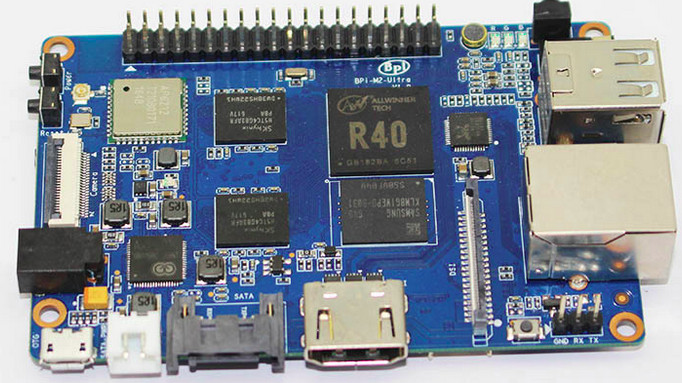
\includegraphics[width=0.85\textwidth]{./07-images/img-Ch4/Banana-PI-M2U-SBC.jpg}}
		\caption{App4-Banana Pi M2U Single Board Computer}
		\label{fig:App4-Banana-PI-M2U-SBC.jpg}
	\end{center}
\end{figure}

\lstset{basicstyle=\ttfamily\small}
%% \lstset{basicstyle=\ttfamily\tiny}
\begin{lstlisting}[breaklines, frame=single, caption={App4-Specifications of Banana Pi M2U SBC Board}, label=App4-Specifications-of -Banana-Pi-M2U-SBC-Board]
Soc 	Allwinner R40/V40
CPU 	quad-core cortex-A7,the most power efficient CPU core 
GPU 	dual-core MALI-400 MP2 and runs at 500MHz, 
GPU provides OpenGL ES 2.0, hardware-accelerated OpenVG, 
1080p45 H.264 high-profile encode and decode.
SDRAM 	2 GB DDR3 with 733MHz\(shared with GPU\)
SATA 	suppoort SATA interface
GPIO 40 Pins Header, 28 x GPIO, for UART, I2C, SPI, PWM, I2S.
On board Network 10/100/1000Mbps Ethernet\(Realtek RTL8211E)
Wifi Module 	WiFi 802.11 b/g/n \(AP 6212 module on board\)
Bluetooth 	BT4.0, Storage MicroSD\(TF\) card, 8GB eMMC 
Display 4-lane MIPI DSI display,or RGB panel, LVDS panel,
Video 	Multi-format FHD video decoding, including Mpeg1/2, 
Mpeg4, H.263, H.264, etc H.264 decode up to 1080P60,support 
Audio outputs 	HDMI, analog audio \(via 3.5 mm TRRS jack\)
Camera 	A CSI input connector Camera:Supports 8-bit YUV422 
CMOS sensor interface,Supports CCIR656 protocol for NTSC, PAL,
Supports 5M pixel camera sensor,Supports video capture 
solution up to 1080p at 30fps
Audio 	input On board microphone
USB 	2 USB 2.0 host, 1 USB 2.0 OTG
Buttons Reset button, Power button, U-boot button
Leds 	Power status Led and RJ45 Led
IR	onboard IR receiver
DC Power 5V/2A with micro USB port
battery	3.7V lithium battery power support
Sizes	85mmX56mm,same size as raspberry pi 3, Weight 40g 
\end{lstlisting}

%================================================		
\clearpage
\pagebreak

\subsection{App4-Beagle-Board xM Single Board Computer}.

\begin{figure}[htbp]
	\begin{center}
		\frame{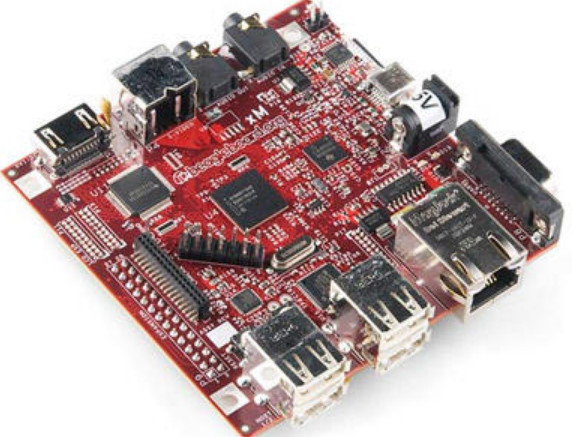
\includegraphics[width=0.85\textwidth]{./07-images/img-Ch4/Beagle-Board-xM-SBC.jpg}}
		\caption{App4-Beagle-Board xM Single Board Computer}
		\label{fig:App4-Beagle-Board-xM-SBC.jpg}
	\end{center}
\end{figure}

\lstset{basicstyle=\ttfamily\small}
%% \lstset{basicstyle=\ttfamily\tiny}
\begin{lstlisting}[breaklines, frame=single, caption={App4-Specifications of Beagle Board xM SBC Board}, label=App4-Specifications-of-Beagle-Board-xM-SBC-Board]
    Processor TI DM3730 Processor 1 GHz ARM Cortex-A8 core
    HD capable TMS320C64x+ core (800 MHz - 720p 30 fps)
    Imagination Technologies PowerVR SGX 2D/3D 
    graphics processor supporting dual independent displays
    512 MB LPDDR RAM, MicroSD/MMC card
    4 GB microSD card supplied with the BeagleBoard-xM 
    and loaded with The Angstrom Distribution
    DVI-D (HDMI connector chosen for size - maximum 
    resolution is 1400x1050)  S-Video
    USB OTG (mini AB), 4 USB ports, Ethernet
    Stereo in and out jacks
    RS-232 port  JTAG connector
    Power socket (5 V barrel connector type)
    Camera port, Expansion port
    Boot code stored on the uSD card, Boot from uSD/MMC only
    Alternative Boot source button.
    Has been demonstrated using Android,[18] 
    Angstrom Linux,[19] Fedora, Ubuntu, Gentoo,
    Arch Linux ARM and Maemo Linux distributions,
    FreeBSD, the Windows CE operating system, and RISC OS.
\end{lstlisting}

%% ===============================================

\begin{flushleft}
\begin{landscape}
%% BEGIN LANDSCAPE ENTIRELY
\pagebreak
\clearpage
%===========================================================
%%% LANDSCAPE BEGINS =======================================
%% \pagebreak
%% \clearpage
%%\begin{flushleft}
%%\begin{landscape}
	
% =========================================================
\subsection{App4-Summary main() function C-Code listing for RTAI}

% ==========================================================
\lstset{basicstyle=\footnotesize, numberstyle=\tiny\color{blue}, frame=single, numbers=left, firstnumber=1, stepnumber=1, numbersep=1pt, xleftmargin=2.0em, framexleftmargin=1.5em, xrightmargin=0.0em, breaklines=true, breakatwhitespace=false, breakindent=5pt, prebreak=\space, postbreak=\space }
% ==========================================================

\begin{lstlisting}[caption={App4-Summary main() function C-Code listing for RTAI}, label=App4-Summary main() function C-Code listing for RTAI]

// File: rtai-CNC14.c
// Date: May 05, 2018 10:04
// Author: WRY
// =========================================================
int main(int argc, char* argv[]) {
// =========================================================
WRY00_Print_DateTime_Usec(); 
printf("Bismillah from WRY executed in main().\n\n");
	
// FOR KEYBOARD INTERRUPT TO STOP (e.g. <Ctrl-C>) EXECUTION
	signal(SIGTERM, WRYcleanup);
	signal(SIGINT,  WRYcleanup);
	signal(SIGKILL, WRYcleanup);
// INVOKE FUNCTIONS SEQUENTIALLY TO RUN RTAI
	system("./load-rtai-modules.sh"); // LOAD RTAI KERNEL MODULES
	WRY01_Create_and_Initialize_Real_Time_Task_LXRT();
	WRY02_Get_Address_and_Name_of_Real_Time_Task_LXRT();
	WRY31_Make_Hard_Real_Timer_Run(); 
	WRY32_Check_Selected_Hard_Real_Time_Run_Mode(); 
	WRY33_Execute_Selected_Hard_Real_Time_Run_Mode();
	WRY04_Allow_NonRoot_Users_For_Hard_Real_Time();
	WRY05_Lock_Memory_Swapping_For_Hard_Real_Time();
	WRY06_ParallelPort_Request_StartUp_and_Enable_IRQ(); 
	WRY07_ParallelPort_Check_RT_Task_Running_Mode();
	WRY08_Start_Run_CNC_Machine();
	WRY09_Stop_Run_CNC_Machine();
	system("./unload-rtai-modules.sh"); // UNLOAD RTAI KERNEL MODULES

WRY00_Print_DateTime_Usec(); 
printf("Alhamdulillah from WRY executed in main().\n"); 
return (0);
}
\end{lstlisting}

\pagebreak
%% =========================================================
\subsection{App4-Full C-Code listing for Real Time (RTAI)}
% ==========================================================
\lstset{basicstyle=\footnotesize, numberstyle=\tiny\color{blue}, frame=single, numbers=left, firstnumber=1, stepnumber=1, numbersep=1pt, xleftmargin=2.0em, framexleftmargin=1.5em, xrightmargin=0.0em, breaklines=true, breakatwhitespace=false, breakindent=5pt, prebreak=\space, postbreak=\space }
% ==========================================================
%% \begin{lstlisting}[caption={Putting listing codes in landscape format}, label=how-to-display-in-landscape]
\begin{lstlisting}[caption={App4-Full C-Code listing for Real Time (RTAI)}, label=App4-Full C-Code listing for Real Time (RTAI)]
// File: rtai-CNC14.c
// Date: May 05, 2018 10:04
// Author: WRY
// 
// =========================================================
// (1) The prefixes WRY and TASK were used extensively in
// order to differentiate our own defined variables and functions 
// from standard C/C++ and RTAI libraries defined variables and functions.
// 
// (2) We must either link our C/C++ program against liblxrt or we 
// have to configure RTAI with "CONFIG_RTAI_LXRT_STATIC_INLINE=y".
// during linux kernel compilation.
//
// =========================================================
// STANDARD C/C++ HEADER FILES USED
// ========================================================= 

	#include <sched.h>	// Scheduler
	#include <stdio.h>	// Standard Input/Output 
	#include <stdlib.h> 	// Standard Library
	#include <time.h>	// For local date-time with usec
	#include <signal.h> 	// Signal for user interrupts, <Ctrl>-C to stop 
	#include <fcntl.h>  	// For file control
	#include <math.h>	// Mathematical functions
	#include <unistd.h> 	// Low level constants, types, function declarations
	#include <errno.h>	// Printing C errors
	#include <string.h>	// Handling strlen IN gcode . h
	#include <curses.h>	// Handling getch () , wgetch ()
	#include <sys/ioctl.h>	// System Input/Output control
	#include <sys/io.h>	// System Input/Output
	#include <sys/mman.h>	// System Memory Manager
	#include <sys/time.h>	// For system local date-time with usec




// ========================================================
// REALTIME HEADER FILES (RTAI)
// ========================================================
	#include <rtai.h>		// RTAI configuration switches (User space and Kernel space)
	#include <rtai_lxrt.h>  	// RTAI User Space libraries

// =========================================================
// RTAI VER. 5.1 DOCUMENTATION REFERENCES
// =========================================================
/*
	For full RTAI Ver 5.1 LOCAL DOCUMENTATION
		file:///usr/realtime/share/doc/rtai-5.1/html/api/files.html
	For <rtai.h>
		file:///usr/realtime/share/doc/rtai-5.1/html/api/rtai_8h_source.html
	For <rtai_lxrt.h>
		file:///usr/realtime/share/doc/rtai-5.1/html/api/rtai__lxrt_8h.html
	For <rtai_sem.h>
		file:///usr/realtime/share/doc/rtai-5.1/html/api/rtai__sem_8h.html
	For <rtai_sched.h>
		file:///usr/realtime/share/doc/rtai-5.1/html/api/rtai__sched_8h_source.html
	For <rtai_usi.h>
		file:///usr/realtime/share/doc/rtai-5.1/html/api/rtai__usi_8h_source.html
*/
// =========================================================
// EXAMPLE USAGE OF RTAI FUNCTIONS (INTERRUPT-BASED)
// ========================================================= 
/*	rt_set_oneshot_mode();
	rt_set_periodic_mode();
	start_rt_timer();
	rt_request_irq_task(PARPORT_IRQ, WRY_RT_task, RT_IRQ_TASK, 1)
	rt_task_init(); 
	rt_task_make_periodic(); 
	rt_make_hard_real_time();
	rt_make_soft_real_time();
	rt_allow_nonroot_hrt();
	rt_task_delete(WRY_RT_task);
	stop_rt_timer();
*/

// ========================================================-
// RTAI DEFINED FUNCTIONS
// =========================================================
/*
	static void * 		rt_get_adr (unsigned long name);
		Get an object address by its name. 
		Returns the address associated to name on success, 0 on failure 
	
	static unsigned long 	rt_get_name (void *adr);
		Get an object name by its address. 
		Returns the address associated to name on success, 0 on failure 
	
	static RT_TASK * 	rt_task_init (unsigned long name, int priority, int stack_size, int max_msg_size);
		Create an RTAI task extension for a Linux process/task in user space.
	
	static void 		rt_make_soft_real_time (void);
		Return a hard real time Linux process, or pthread to the standard Linux behavior.
	
	static void 		rt_make_hard_real_time (void);
		Give a Linux process, or pthread, hard real time execution capabilities allowing full kernel preemption
	
	static void 	rt_allow_nonroot_hrt (void);
		Allows a non root user to use the Linux POSIX soft real time process management and memory lock functions, and allows it to do any input-output operation from user space.
*/
// ========================================================
// GLOBAL DEFINITIONS
// ========================================================
	#define PERIOD		500000		// nanoseconds
	#define TICK_TIME	1000000		// nanoseconds
	// #define CPUMAP 	0xF  		// 16-cpus
	#define CPUMAP		0x4		// 4-cpus
	
	// BUILT_IN PARALLEL PORT ON MOTHERBOARD
	// #define PARPORT_IRQ	7
	// #define BASEPORT	0x378
	
	// HARDWARE 1 = parport0: PC-style at 0xd010 (0xd000), irq 18
	#define BASEPORT	0xd010
	#define PARPORT_IRQ	18

	// HARDWARE 2 = parport1: PC-style at 0xe100, irq 17
	// #define BASEPORT	0xe100
	// #define PARPORT_IRQ	17

	static volatile int ovr, intcnt, retval, maxcnt;

// =========================================================
// HARDWARE DEVICES PARALLEL PORT SEARCH
// =========================================================
/* EXECUTE SYSTEM FUNCTION
root@dell-ub1604-64b:/home/wruslan# dmesg | grep parp

KERNEL MESSAGE - FOUND PARALLEL PORT NO. 1
	[    8.989048] parport0: PC-style at 0xd010 (0xd000), irq 18, using FIFO [PCSPP,TRISTATE,COMPAT,EPP,ECP]
	[    9.089563] lp0: using parport0 (interrupt-driven).
	
KERNEL MESSAGE - FOUND PARALLEL PORT NO. 2
	[   11.972056] parport1: PC-style at 0xe100, irq 17 [PCSPP,TRISTATE]
	[   12.073309] lp1: using parport1 (interrupt-driven).

root@dell-ub1604-64b:/home/wruslan# lspci -v

LIST PCI DEVICE - FOUND PARALLEL PORT NO. 1
	03:00.0 Parallel controller: Oxford Semiconductor Ltd Device c110 (prog-if 02 [ECP])
	Subsystem: Oxford Semiconductor Ltd Device c110
	Flags: bus master, fast devsel, latency 0, IRQ 18
	I/O ports at d010 [size=8]
	I/O ports at d000 [size=4]
	Capabilities: [40] Power Management version 3
	Capabilities: [50] MSI: Enable- Count=1/1 Maskable- 64bit+
	Capabilities: [70] Express Legacy Endpoint, MSI 00
	Capabilities: [100] Device Serial Number 00-30-e0-11-11-00-01-10
	Capabilities: [110] Power Budgeting <?>
	Kernel driver in use: parport_pc
	Kernel modules: parport_pc

	
LIST PCI DEVICE - FOUND PARALLEL PORT NO. 2
	02:00.0 Serial controller: Device 1c00:3250 (rev 10) (prog-if 05 [16850])
	Subsystem: Device 1c00:3250
	Flags: fast devsel, IRQ 17
	I/O ports at e000 [size=256]
	Memory at f0100000 (32-bit, prefetchable) [size=32K]
	I/O ports at e100 [size=4]
	Expansion ROM at f7c00000 [disabled] [size=32K]
	Capabilities: [60] Power Management version 3
	Capabilities: [68] MSI: Enable- Count=1/32 Maskable+ 64bit+
	Capabilities: [80] Express Legacy Endpoint, MSI 00
	Capabilities: [100] Advanced Error Reporting
	Kernel driver in use: parport_serial
	Kernel modules: parport_serial

*/
// ========================================================
// REAL TIME OBJECTS
// ========================================================
	static RT_TASK* 	WRYtask;
	static RT_TASK*     	WRY_RT_task;
	struct sched_param 	WRYsched;
	struct timeval 		WRYstart, WRYfinish;
	unsigned long 		WRY_RT_task_name; 

// ========================================================
// TIMING FOR GENERAL CNC EXECUTION
// ========================================================
	static RTIME 		CNCunixtime1, CNCunixtime2;
	static RTIME		CNCstart_time_ns, CNCcurrent_time_ns;
	static RTIME		CNCend_time_ns, CNCrun_duration_ns;
	static RTIME 		CNCtimer_period_ns; // timer period, in nanoseconds
	RTIME 			CNCtimer_period_count; //actual timer period, in counts




// ========================================================
// TIMING FOR INDIVIDUAL TASK EXECUTION
// ========================================================
	struct timeval 		TASKstart, TASKfinish;
	long int		TASKusec_duration;
	double			TASKsec_duration;

// ========================================================
// GLOBAL VARIABLES (With KEYBOARD Interrupt)
// ========================================================
	int 			WRYpriority     = 0; // Highest
	int 			WRYstack_size   = 0; // Using default (512)
	int 			WRYmax_msg_size = 0; // Using default (256)
	int 			WRYpolicy 	= SCHED_FIFO;
	int 			WRYcpus_allowed	= CPUMAP;
	long int 		WRYusec_duration;
	double 			WRYsec_duration ;
	int			WRYsig;  // Keyboard interrupt signal <Ctrl>-C
	static volatile int 	ovr, intcnt, retval, maxcnt;

// =======================================================
// DEFINE REALTIME TASK STATUS AND SETTINGS
// =======================================================
// REFERNCE: Initially task status set to non-periodic (value non-zero)
// Later on in program we make task periodic (change value to 0)

	int 		WRY_RT_task_status = 1;  
	static RTIME 	WRYexpected;
	static RTIME 	WRYsampling_interval;	

// SELECT REAL TIME TIMER PERIOD
	static RTIME 	CNCtimer_period_ns = 1000*1000*1000; // means (1 sec) period

// SET REAL TIME RUN MODE (BOTH CANNOT BE TRUE)
	int 		WRY_set_periodic_mode = 1; // TRUE  = 1 
	int		WRY_set_one_shot_mode = 0; // FALSE = 0

// SELECTED RUN MODE VALUES (PERIODIC == 1, ONE-SHOT == 2)
	int 		WRY_selected_run_mode; 

// TASK PERIODIC STATUS VALUES (PERIODIC == 0, NON-PERIODIC != 0)
	int 		WRY_task_periodic_status;

// TASK ONE-SHOT STATUS VALUES (ONE-SHOT ???, NON-ONE-SHOT ???)
	int 		WRY_task_one_shot_status;




// =======================================================
// GLOBAL DATA STRUCTURES 
// =======================================================
// Used for WRY00_Print_DateTime_Usec(void) ONLY in order 
// to avoid repetitive declarations (reused) 

	time_t 		WRYtimer;
	char 		WRYbuffer[26];
	struct tm*	WRYtm_info;
	struct timeval	WRYtval_now;




// ========================================================
void WRY00_Print_DateTime_Usec(void) {
// ========================================================
// EXECUTIONS
	time(&WRYtimer);
	WRYtm_info = localtime(&WRYtimer);
	strftime(WRYbuffer, 26, "%Y-%m-%d %H:%M:%S", WRYtm_info);
	gettimeofday(&WRYtval_now, NULL);
	printf("%s", WRYbuffer);
	printf(".%09ld \t", (long int)WRYtval_now.tv_usec);
}




// =======================================================
void WRY01_Create_and_Initialize_Real_Time_Task_LXRT(void) {
// =======================================================
WRY00_Print_DateTime_Usec(); 
printf("STARTED  WRY01_Create_and_Initialize_Real_Time_Task-LXRT(void).\n");

// Create an RTAI task extension for a Linux process/task in user space.

	if (!(WRY_RT_task = rt_task_init(nam2num("CNC06"), WRYpriority, WRYstack_size, WRYmax_msg_size))) {
		WRY00_Print_DateTime_Usec();
		printf("ERROR : Cannot initialize real time task LXRT.\n");
		WRY00_Print_DateTime_Usec();
		printf("ERROR DESCRIPTION : %s\n", strerror(errno));
		exit(1);
	} else {
		WRY00_Print_DateTime_Usec();
		printf("SUCCESS: Completed real time task LXRT initialization.\n");
	}

WRY00_Print_DateTime_Usec(); 
printf("FINISHED WRY01_Create_and_Initialize_Real_Time_Task-LXRT(void).\n\n");
}

// =======================================================
void WRY02_Get_Address_and_Name_of_Real_Time_Task_LXRT(void) {
// =======================================================
WRY00_Print_DateTime_Usec(); 
printf("STARTED  WRY02_Get_Address_and_Name_of_Real_Time_Task_LXRT(void).\n");

	// GET RT_TASK NAME BY ADDRESS
	if (rt_get_name(WRY_RT_task) == 0) {
		WRY00_Print_DateTime_Usec();
		printf("ERROR : Cannot get name of real time task LXRT.\n");
		WRY00_Print_DateTime_Usec();
		printf("ERROR DESCRIPTION : %s\n", strerror(errno));
	//	exit(1);
	} else {
		WRY00_Print_DateTime_Usec();
		printf("SUCCESS: NAME of real time task LXRT = %p\n", (void *)WRY_RT_task);
		WRY_RT_task_name = (unsigned long)WRY_RT_task;
	}

WRY00_Print_DateTime_Usec(); 
printf("FINISHED WRY02_Get_Address_and_Name_of_Real_Time_Task_LXRT(void).\n\n");
}

// ========================================================
void WRY31_Make_Hard_Real_Timer_Run(void) {
// ========================================================
WRY00_Print_DateTime_Usec(); 
printf("STARTED  WRY31_Make_Hard_Real_Timer_Run(void).\n");

	// EXECUTE HARD REAL TIMER CLOCK
	rt_make_hard_real_time();
	
	// IF HARD REAL TIME ALREADY RUNNING, NOTIFY STATUS
	if (rt_is_hard_timer_running()) {
		WRY00_Print_DateTime_Usec();
		printf("SUCCESS: Hard real timer is already running.\n");
	} else {
		// IF NOT RUNNING, START WHILE LOOP
		while (!(rt_is_hard_timer_running())) {
	
			// EXECUTE HARD REAL TIMER CLOCK
			rt_make_hard_real_time();
			// IF HARD REAL TIMER IS NOT RUNNING, THEN RUN IT BY LOOPING.
			if (rt_is_hard_timer_running()) {
				WRY00_Print_DateTime_Usec();
				printf("SUCCESS: Hard real timer is NOW running.\n");
			} else {
				WRY00_Print_DateTime_Usec();
				printf("FAILED : Hard real timer is NOT YET running.\n");
				WRY00_Print_DateTime_Usec();
				printf("ERROR DESCRIPTION : %s\n", strerror(errno));
				// exit(1); // DISABLED TO KEEP ON TRYING
			} END if else    
		} // END while loop
	} // END if else

WRY00_Print_DateTime_Usec(); 
printf("FINISHED WRY31_Make_Hard_Real_Timer_Run(void).\n\n");
}

// ========================================================
void WRY32_Check_Selected_Hard_Real_Time_Run_Mode(void) {
// ========================================================
WRY00_Print_DateTime_Usec(); 
printf("STARTED  WRY32_Check_Selected_Hard_Real_Time_Run_Mode(void).\n");

	// BOTH RUN MODES SELECTED
	if ((WRY_set_periodic_mode == 1) && (WRY_set_one_shot_mode == 1)) {
		WRY00_Print_DateTime_Usec();
		printf("ERROR : Cannot select both periodic_mode and one-shot mode.\n");
		exit(1); 	
		} 
	// NO RUN MODE SELECTED
	if ((WRY_set_periodic_mode == 0) && (WRY_set_one_shot_mode == 0)) {
		WRY00_Print_DateTime_Usec();
		printf("ERROR : No hard realtime run mode selected.\n");
		exit(1); 	
		} 
	// PERIODIC MODE SELECTED
	if ((WRY_set_periodic_mode == 1) && (WRY_set_one_shot_mode == 0)) {
		WRY00_Print_DateTime_Usec();
		printf("SUCCESS: PERIODIC hard realtime run mode selected.\n");
		WRY_selected_run_mode = 1; 	
		} 
	// ONE-SHOT MODE SELECTED
	if ((WRY_set_periodic_mode == 0) && (WRY_set_one_shot_mode == 1)) {
		WRY00_Print_DateTime_Usec();
		printf("SUCCESS: ONE-SHOT hard realtime run mode selected.\n");
		WRY_selected_run_mode = 2;	
		}
WRY00_Print_DateTime_Usec(); 
printf("FINISHED WRY32_Check_Selected_Hard_Real_Time_Run_Mode(void).\n\n");
}

// ========================================================
void WRY33_Execute_Selected_Hard_Real_Time_Run_Mode(void) {
// ========================================================
WRY00_Print_DateTime_Usec(); 
printf("STARTED  WRY33_Execute_Selected_Hard_Real_Time_Run_Mode(void).\n");

	// FOR PERIODIC-MODE REAL TIME RUN
	if (WRY_selected_run_mode == 1) {
	
		WRY00_Print_DateTime_Usec();
		printf("SUCCESS: PERIODIC Set CNCtimer_period_ns \t= %lld \n", CNCtimer_period_ns);
	
		rt_set_periodic_mode();
		WRY00_Print_DateTime_Usec();
		printf("SUCCESS: PERIODIC Execute rt_set_periodic_mode().\n");

		CNCtimer_period_count=nano2count(CNCtimer_period_ns);
		WRY00_Print_DateTime_Usec();
		printf("SUCCESS: PERIODIC Execute nano2count(CNCtimer_period_ns).\n");

		WRY00_Print_DateTime_Usec();
		printf("SUCCESS: PERIODIC CNCtimer_period_count \t= %lld \n", CNCtimer_period_count);

		start_rt_timer(CNCtimer_period_count);
		WRY00_Print_DateTime_Usec();
		printf("SUCCESS: PERIODIC Execute start_rt_timer(CNCtimer_period_count).\n");

		rt_task_make_periodic(WRY_RT_task, WRYexpected, WRYsampling_interval);
		WRY00_Print_DateTime_Usec();
		printf("SUCCESS: PERIODIC Execute rt_task_make_periodic(WRY_RT_task, x, x).\n");

	} // END if PERIODIC-MODE

	// FOR ONE-SHOT MODE REAL TIME RUN
	if (WRY_selected_run_mode == 2) {
	
		rt_set_oneshot_mode();
		WRY00_Print_DateTime_Usec();
		printf("SUCCESS: ONE-SHOT Execute rt_set_oneshot_mode().\n");
		
		start_rt_timer(0);
		WRY00_Print_DateTime_Usec();
		printf("SUCCESS: ONE-SHOT Execute start_rt_timer(0).\n");
	
	} // END if ONE-SHOT MODE

WRY00_Print_DateTime_Usec(); 
printf("FINISHED WRY33_Execute_Selected_Hard_Real_Time_Run_Mode(void).\n\n");
}

// ========================================================
void WRY04_Allow_NonRoot_Users_For_Hard_Real_Time(void) {
// ========================================================
WRY00_Print_DateTime_Usec(); 
printf("STARTED  WRY04_Allow_NonRoot_Users_For_Hard_Real_Time(void).\n");

	// ALLOW NON-ROOT USERS TO HARD REAL TIME
	rt_allow_nonroot_hrt();
	WRY00_Print_DateTime_Usec();
	printf("SUCCESS: Execute Allow hard realtime for non-root users.\n");

WRY00_Print_DateTime_Usec(); 
printf("FINISHED WRY04_Allow_NonRoot_Users_For_Hard_Real_Time(void).\n\n");
}
// ========================================================
void WRY05_Lock_Memory_Swapping_For_Hard_Real_Time(void) {
// ========================================================
WRY00_Print_DateTime_Usec(); 
printf("STARTED  WRY05_Lock_Memory_Swapping_For_Hard_Real_Time(void).\n");

	// LOCK RAM MEMORY FROM MEMORY SWAPPING
	mlockall(MCL_CURRENT | MCL_FUTURE);
	WRY00_Print_DateTime_Usec();
	printf ("SUCCESS: Execute Lock memory and now no memory swapping for hard realtime.\n") ;

WRY00_Print_DateTime_Usec(); 
printf("FINISHED WRY05_Lock_Memory_Swapping_For_Hard_Real_Time(void).\n\n");
}

// ========================================================
void WRY06_ParallelPort_Request_StartUp_and_Enable_IRQ(void) {
// ========================================================
WRY00_Print_DateTime_Usec(); 
printf("STARTED  WRY06_ParallelPort_Request_StartUp_and_Enable_IRQ(void).\n");

	// The name says it, IRQs managed in user space
	// REQUEST IRQ FOR PARALLEL PORT TASK (WRY_RT_task)
		rt_request_irq_task(PARPORT_IRQ, WRY_RT_task, RT_IRQ_TASK, 1);
	
		if(!(rt_request_irq_task(PARPORT_IRQ, WRY_RT_task, RT_IRQ_TASK, 1))) {
			WRY00_Print_DateTime_Usec();
			printf("ERROR  : rt_request_irq_task(PARPORT_IRQ, WRY_RT_task, RT_IRQ_TASK, 1).\n");
			WRY00_Print_DateTime_Usec();
			printf("ERROR DESCRIPTION : %s\n", strerror(errno));
			exit(1); // Commented during testing only
		} else {
			WRY00_Print_DateTime_Usec();
			printf("SUCCESS: Display PARPORT_IRQ \t= %d\n", PARPORT_IRQ);
			
			WRY00_Print_DateTime_Usec();
			printf("SUCCESS: Display RT_IRQ_TASK \t= %d\n", RT_IRQ_TASK);
			
			WRY00_Print_DateTime_Usec();
			printf("SUCCESS: Display BASEPORT \t= 0x%02X\n", BASEPORT);
			
			WRY00_Print_DateTime_Usec();
			printf("SUCCESS: Display CPUMAP \t= 0x%02X\n", CPUMAP);
			
			WRY00_Print_DateTime_Usec();
			printf("SUCCESS: Display PERIOD \t= %d (ns)\n", PERIOD);
			
			WRY00_Print_DateTime_Usec();
			printf("SUCCESS: Display TICK_TIME \t= %d (ns)\n", TICK_TIME);
			
			WRY00_Print_DateTime_Usec();
			printf("SUCCESS: Execute rt_request_irq_task(PARPORT_IRQ, WRY_RT_task, RT_IRQ_TASK, 1).\n");
		} // END if else (rt_request)			


/* REFERENCE NOTES: ===============
		https://www.rtai.org/userfiles/documentation/magma/html/api/group__hal.html#ga74
		
		Often some of the above functions do equivalent things. Once more there is no way of doing it right except by knowing the hardware you are manipulating. Furthermore you must also remember that when you install a hard real time handler the related interrupt is usually disabled, unless you are overtaking one already owned by Linux which has been enabled by it. Recall that if have done it right, and interrupts do not show up, it is likely you have just to rt_enable_irq() your irq. 
		
	TO SOLVE PROBLEM FOR RTAI VER 5.1 = BOTH LINES BELOW ARE NOT NEEDED
		rt_startup_irq(PARPORT_IRQ);
		rt_enable_irq(PARPORT_IRQ);
============== END REFERENCE NOTES */

WRY00_Print_DateTime_Usec(); 
printf("FINISHED WRY06_ParallelPort_Request_StartUp_and_Enable_IRQ(void).\n\n");
}

// ========================================================
void  WRY07_ParallelPort_Check_RT_Task_Running_Mode(void) {
// ========================================================
WRY00_Print_DateTime_Usec(); 
printf("STARTED  WRY07_ParallelPort_Check_RT_Task_Running_Mode(void).\n");

	WRY00_Print_DateTime_Usec();
	printf("SUCCESS: Display WRY_selected_run_mode = %d\n", WRY_selected_run_mode);

	// FOR RUN PERIODIC MODE SELECTED
	if (WRY_selected_run_mode == 1) {
	
		WRY_task_periodic_status = rt_task_make_periodic(WRY_RT_task, WRYexpected, WRYsampling_interval);
	
		// IF TASK RUNNING IN PERIODIC MODE
		if (WRY_task_periodic_status == 0) {  
			WRY00_Print_DateTime_Usec();
			printf("SUCCESS: Display WRY_RT_task is ALREADY running in periodic mode.\n");
		} else {
			// LOOP WHILE NOT RUNNING IN PERIODIC MODE
			// MAKE RT_TASK RUN IN PERIODIC MODE
			while (WRY_task_periodic_status != 0) {  
	
				WRY_task_periodic_status = rt_task_make_periodic(WRY_RT_task, WRYexpected, WRYsampling_interval);
				WRY00_Print_DateTime_Usec();
				printf("SUCCESS: Execute rt_task_make_periodic(WRY_RT_task, WRYexpected, WRYsampling_interval).\n");

				if (WRY_task_periodic_status == 0) {  
					WRY00_Print_DateTime_Usec();
					printf("SUCCESS: Display WRY_RT_task is NOW running in periodic mode.\n");
				} // END if
				
			} // END while loop MAKE TASK PERIODIC
		} // END if..else TASK RUNNING
	} END if SELECTED MODE

/* REFERENCE NOTES: ================

	int rt_task_make_periodic(RT_TASK* task, RTIME start_time, RTIME period) 
		Make a task run periodically.
	
	rt_task_make_periodic mark the task task, previously created with rt_task_init(), as suitable for a periodic execution, with period period, when rt_task_wait_period() is called.
	The time of first execution is defined through start_time or start_delay. start_time is an absolute value measured in clock ticks. start_delay is relative to the current time and measured in nanoseconds.
	
	Parameters:
		task 	is a pointer to the task you want to make periodic.
		start_time 	is the absolute time to wait before the task start running, in clock ticks.
		period 	corresponds to the period of the task, in clock ticks.

	Return values:
		0 	on success. A negative value on failure as described below:
		EINVAL: task does not refer to a valid task.
================== END REFERENCE NOTES  */

WRY00_Print_DateTime_Usec(); 
printf("FINISHED WRY07_ParallelPort_Check_RT_Task_Running_Mode(void).\n\n");
}

// ========================================================
void WRY08_Start_Run_CNC_Machine(void) {
// ========================================================
WRY00_Print_DateTime_Usec(); 
printf("STARTED  WRY08_Start_Run_CNC_Machine(void).\n");

	// MAP START CNC RUNTIME IN NANO SECONDS
	CNCstart_time_ns = rt_get_time_ns();
	WRY00_Print_DateTime_Usec(); 
	printf("SUCCESS: Start CNC run at time \t= %lld (ns)\n", CNCstart_time_ns);

	// EXAMPLE EXECUTE OF CNC Signals File RUN HERE 
	int x; 
	
	// START FOR ... CONTROL LOOP THAT READS CNC SIGNALS FILE AND WRITE LINE-BY-LINE
	// THIS FOR LOOP IS A TEST FOR 10 LINES TO WRITE
	for (x = 0; x < 10; x++) {
		
		// START TIMER
		gettimeofday(&TASKstart, NULL); CNCunixtime1 = rt_get_time_ns();
		
		// EXECUTE TEST RUN IMPORTANT
		// NOTE: rt_sleep suspends execution of the caller task for  a time of delay internal count units. During this time  the CPU is used by other tasks. TIME: 1000000000 (ns) = 2893422000 (internal counts)

		// FOR COMPILATION TESTING ONLY
		// DIFFERENT HARDWARE DEVICES WILL WRITE DIFFERENTLY
		outb_p(25, BASEPORT);   // THIS IS WRITING FOR PARALLEL PORT ON LINUX

		WRY00_Print_DateTime_Usec(); 
		printf("TEST WRITING outb_p(25, BASEPORT) \n");

		// THIS SLEEP TIME IS FOR PUSLE FEEDRATE
		// rt_sleep(1000000000);
		rt_sleep(2893422000);

		WRY00_Print_DateTime_Usec(); 
		printf("run rt_sleep(2893422000) internal counts for x = %d ", x);

		// END TIMER
		CNCunixtime2 = rt_get_time_ns(); gettimeofday(&TASKfinish,NULL);
		printf("run duration = %lld (ns)\n", (CNCunixtime2 - CNCunixtime1));
		
	} // END FOR ... CONTROL LOOP (MEANS G-CODE PROCESSING ENDED)

	CNCend_time_ns = rt_get_time_ns();
	WRY00_Print_DateTime_Usec(); 
	printf("SUCCESS: End CNC run at time \t= %lld (ns)\n", CNCend_time_ns);
	
	CNCrun_duration_ns = (CNCend_time_ns - CNCstart_time_ns);
	WRY00_Print_DateTime_Usec(); 
	printf("SUCCESS: CNC total run duration\t= %lld (ns)\n", CNCrun_duration_ns);


/* REFERENCE NOTES ================= 

	CONSIDER RTAI SLEEP AND 
		rt_get_time_ns();   Nanoseconds timing in RTAI
		rt_sleep(1000000);  Equivalent to 1 second (rt_sleep is defined in micro seconds).
		rt_task_wait_period();
	
	REALTIME DRIVER FOR PARALLEL PORT OUTPUTS, MODIFIED FOR LINUX BY WRY
	REFER: Phase1D-CNC-RTOS - Report Page 161 of 204.
	
	outb_p(valout_pulse + on , BASEPORT);
	usleep(700);
	outb_p(valout_dir + on , BASEPORT);
	usleep(700);
	
	OUTB(2)              Linux Programmer's Manual                OUTB(2)	
	
	NAME
	
	outb, outw, outl, outsb, outsw, outsl, inb, inw, inl, insb, 
	insw, insl, outb_p, outw_p, outl_p, inb_p, inw_p, inl_p - port I/O

	SYNOPSIS
	#include <sys/io.h>

	unsigned char inb(unsigned short int port);
	unsigned char inb_p(unsigned short int port);
	unsigned short int inw(unsigned short int port);
	unsigned short int inw_p(unsigned short int port);
	unsigned int inl(unsigned short int port);
	unsigned int inl_p(unsigned short int port);

	void outb(unsigned char value, unsigned short int port);
	void outb_p(unsigned char value, unsigned short int port);
	void outw(unsigned short int value, unsigned short int port);
	void outw_p(unsigned short int value, unsigned short int port);
	void outl(unsigned int value, unsigned short int port);
	void outl_p(unsigned int value, unsigned short int port);

	void insb(unsigned short int port, void *addr,
	unsigned long int count);
	void insw(unsigned short int port, void *addr,
	unsigned long int count);
	void insl(unsigned short int port, void *addr,
	unsigned long int count);
	void outsb(unsigned short int port, const void *addr,
	unsigned long int count);
	void outsw(unsigned short int port, const void *addr,
	unsigned long int count);
	void outsl(unsigned short int port, const void *addr,
	unsigned long int count);

================== END REFERENCE NOTES */

WRY00_Print_DateTime_Usec(); 
printf("FINISHED WRY08_Start_Run_CNC_Machine(void).\n\n");
}

// =======================================================
void WRY09_Stop_Run_CNC_Machine(void) {
// ========================================================
WRY00_Print_DateTime_Usec(); 
printf("STARTED  WRY09_Stop_Run_CNC_Machine(void).\n");

	// RELEASE PARALLEL PORT 
	rt_release_irq_task(PARPORT_IRQ);
	WRY00_Print_DateTime_Usec(); 
	printf("SUCCESS: Execute rt_release_irq_task(PARPORT_IRQ).\n");
	
	// STOP REALTIME TIMER
	stop_rt_timer();
	WRY00_Print_DateTime_Usec(); 
	printf("SUCCESS: Execute stop_rt_timer().\n");
	
	// REVERT TO SOFT REALTIME
	rt_make_soft_real_time();
	WRY00_Print_DateTime_Usec(); 
	printf("SUCCESS: Execute rt_make_soft_real_time().\n");
	
	// DELETE REALTIME TASK
	rt_task_delete(WRY_RT_task);
	WRY00_Print_DateTime_Usec(); 
	printf("SUCCESS: Execute rt_task_delete(WRY_RT_task).\n");
	
	// NORMAL PROGRAM TERMINATION
	WRY00_Print_DateTime_Usec(); 
	printf("SUCCESS: Finished cleanup. Exiting program normally.\n");

WRY00_Print_DateTime_Usec(); 
printf("FINISHED WRY09_Stop_Run_CNC_Machine(void).\n\n");
}

// ========================================================
void WRYcleanup(int WRYsig) {
// ========================================================
printf("\n\n");
WRY00_Print_DateTime_Usec(); 
printf("STARTED  USER INTERRUPT RESPONSE TO STOP.\n");

	WRY00_Print_DateTime_Usec(); 
	printf("SUCCESS: Activate stop on User <Ctrl>-C Interrupt.\n");
	WRY00_Print_DateTime_Usec(); 
	printf("SUCCESS: Start cleanup sequence to exit program.\n");
	
	// RELEASE PARALLEL PORT 
	rt_release_irq_task(PARPORT_IRQ);
	WRY00_Print_DateTime_Usec(); 
	printf("SUCCESS: Execute rt_release_irq_task(PARPORT_IRQ).\n");
	
	// STOP REALTIME TIMER
	stop_rt_timer();
	WRY00_Print_DateTime_Usec(); 
	printf("SUCCESS: Execute stop_rt_timer().\n");
	
	// REVERT TO SOFT REALTIME
	rt_make_soft_real_time();
	WRY00_Print_DateTime_Usec(); 
	printf("SUCCESS: Execute rt_make_soft_real_time().\n");
	
	// ABNORMAL TERMINATION
	WRY00_Print_DateTime_Usec(); 
	printf("SUCCESS: Abnormal termination. Finished cleanup. Exiting program.\n");
	WRY00_Print_DateTime_Usec(); 
	printf("FINISHED USER INTERRUPT RESPONSE TO STOP.\n");
	
	// DELETE REALTIME TASK
	WRY00_Print_DateTime_Usec(); 
	printf("SUCCESS: Execute rt_task_delete(WRY_RT_task).\n\n");
	rt_task_delete(WRY_RT_task);

exit(1); // QUIT BASED ON KEYBOARD <Ctrl-C>
}




// ======================================================== 
int main(int argc, char* argv[]) {
// ========================================================
WRY00_Print_DateTime_Usec(); 
printf("Bismillah from WRY executed in main().\n\n");

// TO DO: TO INCLUDE AUTOMATIC RTAI MODULES load/unload

	// system("./load-rtai-modules.sh");
	
// FOR KEYBOARD INTERRUPT TO STOP (e.g. <Ctrl-C>)
	signal(SIGTERM, WRYcleanup);
	signal(SIGINT,  WRYcleanup);
	signal(SIGKILL, WRYcleanup);
	
// INVOKE FUNCTIONS SEQUENTIALLY TO RUN RTAI
	WRY01_Create_and_Initialize_Real_Time_Task_LXRT();
	WRY02_Get_Address_and_Name_of_Real_Time_Task_LXRT();
	WRY31_Make_Hard_Real_Timer_Run(); 
	WRY32_Check_Selected_Hard_Real_Time_Run_Mode(); 
	WRY33_Execute_Selected_Hard_Real_Time_Run_Mode();
	WRY04_Allow_NonRoot_Users_For_Hard_Real_Time();
	WRY05_Lock_Memory_Swapping_For_Hard_Real_Time();
	WRY06_ParallelPort_Request_StartUp_and_Enable_IRQ(); 
	WRY07_ParallelPort_Check_RT_Task_Running_Mode();
	WRY08_Start_Run_CNC_Machine();
	WRY09_Stop_Run_CNC_Machine();
	
	//system("./unload-rtai-modules.sh");

WRY00_Print_DateTime_Usec(); 
printf("Alhamdulillah from WRY executed in main().\n"); 
return (0);
}

// ======================================================
\end{lstlisting}

% =========================================================
% ============== BELOW IMPT TO MATCH \begin with \end ===== 
% \end{landscape}
% \end{flushleft}
% \clearpage
\pagebreak
% ==================== END OF PAGE ========================

% ==================== START OF PAGE ======================
% \pagebreak
% \clearpage
% \begin{flushleft}
%% \begin{landscape}
% =========================================================
\subsection{App4-Full execution C/C++ code for Real Time (RTAI)}
% ==========================================================
\lstset{basicstyle=\footnotesize, numberstyle=\tiny\color{blue}, frame=single, numbers=left, firstnumber=1, stepnumber=1, numbersep=1pt, xleftmargin=2.0em, framexleftmargin=1.5em, xrightmargin=0.0em, breaklines=true, breakatwhitespace=false, breakindent=5pt, prebreak=\space, postbreak=\space }
% ==========================================================
%% \begin{lstlisting}[caption={Putting listing codes in landscape format}, label=how-to-display-in-landscape]
\begin{lstlisting}[caption={App4-Full execution C/C++ code for Real Time (RTAI)}, label=App4-Full execution C/C++ code for Real Time (RTAI)]
/* COMPILATION AND EXECUTION RESULTS

(1) COMPILATION
wruslan@dell-ub1604-64b:~/ump-project2/test14$ gcc -I./ -I/usr/realtime/include -O2 -pipe -L/usr/realtime/lib -lpthread -llxrt -lm -o rtai-CNC14.x rtai-CNC14.c
wruslan@dell-ub1604-64b:~/ump-project2/test14$

(2) DISPLAY COMPILED EXECUTABLE 
wruslan@dell-ub1604-64b:~/ump-project2/test14$ ls -al
total 72
drwxrwxr-x  2 wruslan wruslan  4096 May  2 19:59 .
drwxrwxr-x 19 wruslan wruslan  4096 May  2 19:42 ..
-rwxrwxrwx  1 wruslan wruslan  4096 Apr 28 09:23 load-rtai-modules.sh
-rw-rw-r--  1 wruslan wruslan 31513 May  2 19:59 rtai-CNC14.c
-rwxrwxr-x  1 wruslan wruslan 24064 May  2 19:59 rtai-CNC14.x           <==== FOUND COMPILED EXECUTABLE
-rwxrwxrwx  1 wruslan wruslan  4063 Apr 28 09:28 unload-rtai-modules.sh
wruslan@dell-ub1604-64b:~/ump-project2/test14$

(3) EXECUTE COMPILED EXECUTABLE AS ROOT USER
wruslan@dell-ub1604-64b:~/ump-project2/test14$ sudo ./rtai-CNC14.x 
[sudo] password for wruslan: 
2018-05-02 19:59:42.000944348 	Bismillah from WRY executed in main().

2018-05-02 19:59:42.000945009 	SUCCESS: Completed real time task LXRT initialization.
2018-05-02 19:59:42.000945019 	SUCCESS: NAME of real time task LXRT = 0xffffa08f43997230
2018-05-02 19:59:42.000945038 	SUCCESS: Hard real timer is already running.
2018-05-02 19:59:42.000945045 	SUCCESS: PERIODIC hard realtime run mode selected.
2018-05-02 19:59:42.000945051 	SUCCESS: PERIODIC Set CNCtimer_period_ns 	= 1000000000 
2018-05-02 19:59:42.000945064 	SUCCESS: PERIODIC Execute rt_set_periodic_mode().
2018-05-02 19:59:42.000945076 	SUCCESS: PERIODIC Execute nano2count(CNCtimer_period_ns).
2018-05-02 19:59:42.000945083 	SUCCESS: PERIODIC CNCtimer_period_count 	= 3292519000 
2018-05-02 19:59:42.000945102 	SUCCESS: PERIODIC Execute start_rt_timer(CNCtimer_period_count).
2018-05-02 19:59:42.000945115 	SUCCESS: PERIODIC Execute rt_task_make_periodic(WRY_RT_task, x, x).
2018-05-02 19:59:42.000945128 	SUCCESS: Execute Allow hard realtime for non-root users.
2018-05-02 19:59:42.000945274 	SUCCESS: Execute Lock memory and now no memory swapping for hard realtime.
2018-05-02 19:59:42.000945281 	FINISHED WRY05_Lock_Memory_Swapping_For_Hard_Real_Time(void).

2018-05-02 19:59:42.000945288 	STARTED  WRY06_ParallelPort_Request_StartUp_and_Enable_IRQ(void).
2018-05-02 19:59:42.000945301 	SUCCESS: Display PARPORT_IRQ 	= 18
2018-05-02 19:59:42.000945308 	SUCCESS: Display RT_IRQ_TASK 	= 0
2018-05-02 19:59:42.000945315 	SUCCESS: Display BASEPORT 	= 0xD010
2018-05-02 19:59:42.000945322 	SUCCESS: Display CPUMAP 	= 0x04
2018-05-02 19:59:42.000945329 	SUCCESS: Display PERIOD 	= 500000 (ns)
2018-05-02 19:59:42.000945335 	SUCCESS: Display TICK_TIME 	= 1000000 (ns)
2018-05-02 19:59:42.000945342 	SUCCESS: Execute rt_request_irq_task(PARPORT_IRQ, WRY_RT_task, RT_IRQ_TASK, 1).
2018-05-02 19:59:42.000945348 	FINISHED WRY06_ParallelPort_Request_StartUp_and_Enable_IRQ(void).

2018-05-02 19:59:42.000945355 	STARTED  WRY07_ParallelPort_Check_RT_Task_Running_Mode(void).
2018-05-02 19:59:42.000945362 	SUCCESS: Display WRY_selected_run_mode = 1
2018-05-02 19:59:42.000945374 	SUCCESS: Display WRY_RT_task is ALREADY running in periodic mode.
2018-05-02 19:59:42.000945381 	FINISHED WRY07_ParallelPort_Check_RT_Task_Running_Mode(void).

2018-05-02 19:59:42.000945388 	STARTED  WRY08_Start_Run_CNC_Machine(void).
2018-05-02 19:59:42.000945400 	SUCCESS: Start CNC run at time 	= 1528453940458 (ns)
2018-05-02 19:59:42.000945418 	TEST WRITING outb_p(25, BASEPORT) 
2018-05-02 19:59:43.000824252 	run rt_sleep(2893422000) internal counts for x = 0 run duration = 878838671 (ns)
2018-05-02 19:59:43.000824285 	TEST WRITING outb_p(25, BASEPORT) 
2018-05-02 19:59:44.000703121 	run rt_sleep(2893422000) internal counts for x = 1 run duration = 878841400 (ns)
2018-05-02 19:59:44.000703155 	TEST WRITING outb_p(25, BASEPORT) 
2018-05-02 19:59:45.000581988 	run rt_sleep(2893422000) internal counts for x = 2 run duration = 878838807 (ns)
2018-05-02 19:59:45.000582021 	TEST WRITING outb_p(25, BASEPORT) 
2018-05-02 19:59:46.000460855 	run rt_sleep(2893422000) internal counts for x = 3 run duration = 878839578 (ns)
2018-05-02 19:59:46.000460888 	TEST WRITING outb_p(25, BASEPORT) 
2018-05-02 19:59:47.000339721 	run rt_sleep(2893422000) internal counts for x = 4 run duration = 878838160 (ns)
2018-05-02 19:59:47.000339753 	TEST WRITING outb_p(25, BASEPORT) 
2018-05-02 19:59:48.000218585 	run rt_sleep(2893422000) internal counts for x = 5 run duration = 878836793 (ns)
2018-05-02 19:59:48.000218617 	TEST WRITING outb_p(25, BASEPORT) 
2018-05-02 19:59:49.000097453 	run rt_sleep(2893422000) internal counts for x = 6 run duration = 878841787 (ns)
2018-05-02 19:59:49.000097487 	TEST WRITING outb_p(25, BASEPORT) 
2018-05-02 19:59:49.000976322 	run rt_sleep(2893422000) internal counts for x = 7 run duration = 878839913 (ns)
2018-05-02 19:59:49.000976355 	TEST WRITING outb_p(25, BASEPORT) 
2018-05-02 19:59:50.000855191 	run rt_sleep(2893422000) internal counts for x = 8 run duration = 878840543 (ns)
2018-05-02 19:59:50.000855223 	TEST WRITING outb_p(25, BASEPORT) 
2018-05-02 19:59:51.000734055 	run rt_sleep(2893422000) internal counts for x = 9 run duration = 878835850 (ns)
2018-05-02 19:59:51.000734082 	SUCCESS: End CNC run at time 	= 1537242485990 (ns)
2018-05-02 19:59:51.000734090 	SUCCESS: CNC total run duration	= 8788545532 (ns)
2018-05-02 19:59:51.000734097 	FINISHED WRY08_Start_Run_CNC_Machine(void).

2018-05-02 19:59:51.000734104 	STARTED  WRY09_Stop_Run_CNC_Machine(void).
2018-05-02 19:59:51.000734116 	SUCCESS: Execute rt_release_irq_task(PARPORT_IRQ).
2018-05-02 19:59:51.000734131 	SUCCESS: Execute stop_rt_timer().
2018-05-02 19:59:51.000734141 	SUCCESS: Execute rt_make_soft_real_time().
2018-05-02 19:59:51.000734150 	SUCCESS: Execute rt_task_delete(WRY_RT_task).
2018-05-02 19:59:51.000734156 	SUCCESS: Finished cleanup. Exiting program normally.
2018-05-02 19:59:51.000734162 	FINISHED WRY09_Stop_Run_CNC_Machine(void).

2018-05-02 19:59:51.000734171 	Alhamdulillah from WRY executed in main().
wruslan@dell-ub1604-64b:~/ump-project2/test14$ 
*/
\end{lstlisting}

% =========================================================
%\end{landscape}
%\end{flushleft}



\pagebreak
\clearpage
% ==========================================================
%%% LANDSCAPE BEGINS =======================================
% \pagebreak
% \clearpage
%\begin{flushleft}
%\begin{landscape}

% =========================================================
\subsection{App4-C++2011 Example Parallel Multithreading}
% =========================================================

\begin{enumerate}
	\item The C++ language offers for the first time support in implementing applications that require concurrent programming, regardless of the development platform. 
	
	\item Before the C++11 standard the multi-threaded applications were based on platform-specific extensions, like Intel TBB, OpenMP, Pthreads, etc. Portable applications are the major advantage brought by this new feature (i.e. Windows multi-threaded applications are easily ported to iPhone or Android platforms). 
	
	\item An advantage for those familiariazed with the Boost thread library is that many concepts from the standard C++11 library keep the same name and structure as the boost threads library classes.
	
	\item The C++ Standard Library includes classes for thread manipulation and synchronization, common protected data and low-level atomic operations. We will next exemplify and provide a general description of how these concepts occur in the C++11 Standard.
	
	\item REFERENCE: http://en.cppreference.com/w/cpp/thread
	
	\item COMPILATION \\
	Terminal\$ g++ -o multi-threaded.xx multi-threaded.cpp -std=c++11 -pthread -D\_GLIBCXX\_USE\_NANOSLEEP 
	
	\item EXECUTION\\
	Terminal\$ ./multi-threaded.xx 
	
\end{enumerate}
The 01-multi-threaded C++ program operations are described as follows: 
\begin{enumerate}
	
	\item The main C++ program spawn three threads.
	
	\item Thread-1 sleeps for 10 seconds.
	\item Thread-2 sleeps for  5 seconds.
	\item Thread-3 sleeps for  7 seconds.
	
	\item Thread-1, Thread-2 and Thread-3 are made to run some arbitrary computations to show that individual threads can do some actual useful work. For demonstration, we created three simple functions, one for each thread.  
	
	\item The sleep times were assigned to the threads to actually simulate real conditions where actual threads spent times equal to their sleep times when running actual computations. This is used to prove the time parallel nature in executions of threads.   
	
\end{enumerate}

% ==========================================================
\lstset{basicstyle=\footnotesize, numberstyle=\tiny\color{blue}, frame=single, numbers=left, firstnumber=1, stepnumber=1, numbersep=1pt, xleftmargin=2.0em, framexleftmargin=1.5em, xrightmargin=0.0em, breaklines=true, breakatwhitespace=false, breakindent=5pt, prebreak=\space, postbreak=\space }
% ==========================================================

\begin{lstlisting}[caption={App4-C++2011 Example Parallel Multithreading}, label=App4-C++2011 Example Parallel Multithreading]

// File: independent-parallel-threads-06.cpp
// Date : Sun Mar  8 12:15:41 MYT 2015 
// Author: WRY

// http://en.cppreference.com/w/cpp/thread

// COMPILATION
// THIS DOES NOT WORK
// g++  -o independent-parallel-threads-06.xx independent-parallel-threads-06.cpp -std=c++11 -pthread 

// THE FOLLOWING WORKS
// g++  -o independent-parallel-threads-06.xx independent-parallel-threads-06.cpp -std=c++11 -pthread -D_GLIBCXX_USE_NANOSLEEP 
// g++  -o independent-parallel-threads-06.xx independent-parallel-threads-06.cpp -std=gnu++11 -pthread -D_GLIBCXX_USE_NANOSLEEP 

// =========================================================

	#include <stdio.h>       // To use printf()
	#include <iostream>      // std::cout
	#include <thread>        // std::thread
	#include <ctime>	 // To use the C++ timer function
	#include <chrono>	 // To use the system_clock
	#include <mutex>	 // To run mutual exclusion (mutex) locking thread
	
	using namespace std;

// Global variables (shared among all threads for Read/Write)
	double result_wry_thread_01 = 0.0;
	double result_wry_thread_02 = 0.0;
	double result_wry_thread_03 = 0.0;
	double result_total = 0.0;

// ======================================================== 
void calculate_norm1(double x, double y, double z) {
// ========================================================
// OPENING THREAD
	std::thread::id this_id = std::this_thread::get_id();
	auto threadstart_time = std::chrono::high_resolution_clock::now();
	printf(" %lld Start wry_thread_01. Thread_ID = %x Hex. \n", threadstart_time, this_id);

// PROCESSING THREAD - DELAY (SLEEP) 10 SECONDS
	int sleep_seconds = 10;
	printf(" %lld PROCESSING wry_thread_01. Will sleep for %d seconds ... \n", threadstart_time, sleep_seconds);
	
	std::mutex g_display_mutex;
	g_display_mutex.lock();
	std::this_thread::sleep_for(std::chrono::seconds(sleep_seconds));
	g_display_mutex.unlock();
	
	result_wry_thread_01 = (x + y + z);

// CLOSING THREAD
	auto threadend_time = std::chrono::high_resolution_clock::now();
	auto duration_time = (threadend_time - threadstart_time);
	typedef std::chrono::duration<double> double_seconds;
	double process_seconds = std::chrono::duration_cast<double_seconds>(duration_time).count();
	printf(" %lld Ended wry_thread_01. Thread_ID = %x Hex. Thread processing time = %lf seconds = %lld ticks \n", threadend_time, this_id, process_seconds, duration_time);
}
// ======================================================== 
void calculate_norm2(double x, double y, double z) {
// ========================================================
// OPENING THREAD
	std::thread::id this_id = std::this_thread::get_id();
	auto threadstart_time = std::chrono::high_resolution_clock::now();
	printf(" %lld Start wry_thread_02. Thread_ID = %x Hex. \n", threadstart_time, this_id);

// PROCESSING THREAD - DELAY (SLEEP) 5 SECONDS
	int sleep_seconds = 5;
	printf(" %lld PROCESSING wry_thread_02. Will sleep for %d seconds ... \n", threadstart_time, sleep_seconds);
	
	std::mutex g_display_mutex;
	g_display_mutex.lock();
	std::this_thread::sleep_for(std::chrono::seconds(sleep_seconds));
	g_display_mutex.unlock();
	
	result_wry_thread_02 = (x/0.675 + 15.198*y + 0.005*z);    

// CLOSING THREAD
	auto threadend_time = std::chrono::high_resolution_clock::now();
	auto duration_time = (threadend_time - threadstart_time);
	typedef std::chrono::duration<double> double_seconds;
	double process_seconds = std::chrono::duration_cast<double_seconds>(duration_time).count();
	printf(" %lld Ended wry_thread_02. Thread_ID = %x Hex. Thread processing time = %lf seconds = %lld ticks \n", threadend_time, this_id, process_seconds, duration_time);
}
// ======================================================== 
void calculate_norm3(double x, double y, double z) {
// ========================================================
// OPENING THREAD
	std::thread::id this_id = std::this_thread::get_id();
	auto threadstart_time = std::chrono::high_resolution_clock::now();
	printf(" %lld Start wry_thread_03. Thread_ID = %x Hex. \n", threadstart_time, this_id);

// PROCESSING THREAD - DELAY (SLEEP) 7 SECONDS
	int sleep_seconds = 7;
	printf(" %lld PROCESSING wry_thread_03. Will sleep for %d seconds ... \n", threadstart_time, sleep_seconds);
	
	std::mutex g_display_mutex;
	g_display_mutex.lock();
	std::this_thread::sleep_for(std::chrono::seconds(sleep_seconds));
	g_display_mutex.unlock();
	
	result_wry_thread_03 = (2.56*x + y/1.56 + z*0.017); 

// CLOSING THREAD
	auto threadend_time = std::chrono::high_resolution_clock::now();
	auto duration_time = (threadend_time - threadstart_time);
	typedef std::chrono::duration<double> double_seconds;
	double process_seconds = std::chrono::duration_cast<double_seconds>(duration_time).count();
	printf(" %lld Ended wry_thread_03. Thread_ID = %x Hex. Thread processing time = %lf seconds = %lld ticks \n", threadend_time, this_id, process_seconds, duration_time);
}

// ========================================================
void print_current_date_time() {
// ========================================================
	time_t the_time;
	auto now = std::chrono::system_clock::now();
	the_time = std::chrono::system_clock::to_time_t(now);
	// std::cout << "Now : " << ctime(&tt) << std::endl;
	printf("Date Time: %s", ctime(&the_time));
}

// ========================================================
void time_ticks() {
// ========================================================
	auto ticks_wry = std::chrono::high_resolution_clock::now();
	printf(" %lld ", ticks_wry);
}

// ========================================================
int main(int argc, char *argv[]) {
// ========================================================

// OPENING MAIN PROGRAM MESSAGE
	auto start_time = std::chrono::high_resolution_clock::now();
	time_ticks(); print_current_date_time();
	time_ticks(); printf("Bismillah. Main thread started. \n");

// Threads are started by defining an object std::thread
// Spawn and launch three different threads runnung the same function
	std::thread 	wry_thread_01(calculate_norm1, 1.0, 2.0, 3.0);     
	std::thread 	wry_thread_02(calculate_norm2, 4.0, 5.0, 6.0);        
	std::thread 	wry_thread_03(calculate_norm3, 2.2, 3.2, 6.2);    

// join() - The function returns when the thread execution has completed.
// Synchronize all threads, pause until all threads finish execution.
	wry_thread_01.join();
	wry_thread_02.join();
	wry_thread_03.join();

// DISPLAY RESULTS OF INDIVIDUAL THREADS
	time_ticks(); printf("result_wry_thread_01 = %f \n", result_wry_thread_01);
	time_ticks(); printf("result_wry_thread_02 = %f \n", result_wry_thread_02);
	time_ticks(); printf("result_wry_thread_03 = %f \n", result_wry_thread_03);
	
	time_ticks(); printf("result_total = %f \n", result_wry_thread_01 + result_wry_thread_02 + result_wry_thread_03);

// CALCULATE TOTAL PROCESSING TIME
	auto end_time = std::chrono::high_resolution_clock::now();
	auto duration_time = (end_time - start_time);
	typedef std::chrono::duration<double> double_seconds;
	double process_seconds = std::chrono::duration_cast<double_seconds>(duration_time).count();
	time_ticks(); printf("TOTAL PROGRAM MULTI-THREADED PROCESSING TIME = %lf seconds = %lld ticks. \n", process_seconds, duration_time);

// CLOSING MAIN PROGRAM MESSAGE
	time_ticks(); print_current_date_time();
	time_ticks(); printf("Alhamdulillah. Main thread ended. \n");

return 0;
}
// ========================================================
\end{lstlisting}

\pagebreak
% =========================================================
\subsection{App4-C++2011 Execution Parallel Multithreading}

% ==========================================================
\lstset{basicstyle=\footnotesize, numberstyle=\tiny\color{blue}, frame=single, numbers=left, firstnumber=1, stepnumber=1, numbersep=1pt, xleftmargin=2.0em, framexleftmargin=1.5em, xrightmargin=0.0em, breaklines=true, breakatwhitespace=false, breakindent=5pt, prebreak=\space, postbreak=\space }
% ==========================================================

\begin{lstlisting}[caption={App4-C++2011 Execution Parallel Multithreading}, label=App4-C++2011 Execution Parallel Multithreading]

COMPILATION
===============
root@hpcompaqdk-ub1004-rtai:~/Documents/Multithreaded-C++11/test2.6# g++  -o independent-parallel-threads-06.xx independent-parallel-threads-06.cpp -std=c++11 -pthread -D_GLIBCXX_USE_NANOSLEEP 

EXECUTION
===============
root@hpcompaqdk-ub1004-rtai:~/Documents/Multithreaded-C++11/test2.6# ./independent-parallel-threads-06.xx 
1425871390235109 Date Time: Mon Mar  9 11:23:10 2015
1425871390235280 Bismillah. Main thread started. 
1425871390235345 Start wry_thread_02. Thread_ID = b6f28b70 Hex. 
1425871390235345 PROCESSING wry_thread_02. Will sleep for 5 seconds ... 
1425871390235340 Start wry_thread_01. Thread_ID = b7729b70 Hex. 
1425871390235340 PROCESSING wry_thread_01. Will sleep for 10 seconds ... 
1425871390235398 Start wry_thread_03. Thread_ID = b6727b70 Hex. 
1425871390235398 PROCESSING wry_thread_03. Will sleep for 7 seconds ... 
1425871395235469 Ended wry_thread_02. Thread_ID = b6f28b70 Hex. Thread processing time = 5.000124 seconds = 5000124 ticks 
1425871397235500 Ended wry_thread_03. Thread_ID = b6727b70 Hex. Thread processing time = 7.000102 seconds = 7000102 ticks 
1425871400235832 Ended wry_thread_01. Thread_ID = b7729b70 Hex. Thread processing time = 10.000492 seconds = 10000492 ticks 
1425871400235899 result_wry_thread_01 = 6.000000 
1425871400235922 result_wry_thread_02 = 81.945926 
1425871400235932 result_wry_thread_03 = 7.788682 
1425871400235939 result_total = 95.734608 
1425871400235963 TOTAL PROGRAM MULTI-THREADED PROCESSING TIME = 10.000849 seconds = 10000849 ticks. 
1425871400235969 Date Time: Mon Mar  9 11:23:20 2015
1425871400235995 Alhamdulillah. Main thread ended. 
root@hpcompaqdk-ub1004-rtai:~/Documents/Multithreaded-C++11/test2.6# 
*/
\end{lstlisting}

\pagebreak
% =========================================================
\subsection{App4-C++-MPI Example Parallel Multiprocessing}

\begin{enumerate}
	\item The 03-multi-processing.cpp C++ program is a program based on the OpenMPI library for multi-processing.
	
	\item It requires the installation of this OpenMPI libraries and executables on the particular platform.
	
	\begin{enumerate}
		
		\item COMPILATION:\\ 
		/usr/bin/mpic++ -o 03-multi-processing.xx 03-multi-processing.cpp -lpthread
		
		\item EXECUTION:\\
		/usr/bin/mpirun -np 10 03-multi-processing.xx | sort
		
		\item The number of processes to execute np above is 10. It can be changed by the user to any number preferred.
		
	\end{enumerate}
	
	\item Stage 1 : The program calculates the function kuntakinte(x), where x is an integer put as a very large number like 1000000 (one million).
	
	\item Stage 2 : The program calculates the function kamikamu(x), which is the cumulative sum of kuntakinta(x) which is the sum of kuntakinte(1) + kuntakinte(2) + kuntakinte(3) + .... + kuntakinte(x)
	
	\item The calculation of the function kuntakinta(x) itself is very CPU intensive. Study the program code for kuntakinte() function.
	
	\item The computation strategy for this OpenMPI program is "divide and conquer". Break the execution into np individual processes (multi-processing) to handle the large computation. Split the data regions for x into (x/np) individual tasks. This task is then assign to a process.
	
	\item For example, if x = 1,000,000 (one million), and np = 10, then each process will handle (1,000,000)/10 = 100,000 (one hundred thousand).
	
	\item The final result for kamikamu(1,000,000), as an example, must be the same whether we run with np=5, np=10, np=20 or any integer number because np is just the number of processes we choose to split the computation work.
	
	\item Yes. We have proven that it gave the same results for different values of np.
	
	\item The concept is similar to counting a very large pile (mountain) of oranges. The total count must be the same whether we hire 10 people, 50 people or 100 people to do the counting. The total sum cannot change. 
	
	\item This is what the current OpenMPI code 03-multi-processing.cpp does. The number of people (processes) to do the counting (computation) is np. Ha ha ha. Ya ya ya. Kah kah kah.
	
\end{enumerate}

% ==========================================================
\lstset{basicstyle=\footnotesize, numberstyle=\tiny\color{blue}, frame=single, numbers=left, firstnumber=1, stepnumber=1, numbersep=1pt, xleftmargin=2.0em, framexleftmargin=1.5em, xrightmargin=0.0em, breaklines=true, breakatwhitespace=false, breakindent=5pt, prebreak=\space, postbreak=\space }
% ==========================================================

\begin{lstlisting}[caption={App4-C++-MPI Example Parallel Multiprocessing}, label=App4-C++-MPI Example Parallel Multiprocessing]

// File: kamikamu-parallel.c
// Date: Thu Jan  3 21:53:17 MYT 2013
// Rev1: Mon Nov 18 03:45:54 MYT 2013
//
// This is a kamikamu() and kuntakinte() C-program for running parallel OpenMPI routines 
// that run on a local multicore computer or distributed on a computing cluster. 
//
// COMPILATION 
// /opt/openmpi/bin/mpicc -o kamikamu-parallel.x kamikamu-parallel.c 
// /usr/bin/mpicc -o kamikamu-parallel.x kamikamu-parallel.c 

// EXECUTION ON LOCAL MACHINE
// /opt/openmpi/bin/mpirun -np 10 kamikamu-parallel.x | sort
// /usr/bin/mpirun -np 10 kamikamu-parallel.x | sort

// EXECUTION ON CLUSTER MACHINE
// /opt/openmpi/bin/mpirun -np 10 -hostfile machines kamikamu-parallel.x | sort

// ========================================================
#include <math.h>     // For mathematical functions
#include <stdio.h>    // For function printf()
#include <stdlib.h>   // For function calloc()
#include <string.h>   // For function %s (printf string)
#include <time.h>     // For datetimestamp() function

// SET THE PATH FOR THIS HEADER FILE TO SUIT ITS LOCATION ON YOUR COMPUTER

// #include "/opt/openmpi/include/mpi.h"
#include "/usr/lib/openmpi/include/mpi.h"

// ========================================================
void datetimestamp() {
// ========================================================
	time_t ltime; 		/* calendar time */
	ltime=time(NULL); 	/* get current cal time */
	printf("%s",asctime(localtime(&ltime)));
}
// =========================================================
// DEFINE FUNCTION kuntakinte(n) THE FUNNY FUNCTION
// =========================================================
	unsigned long int kuntakinte(unsigned long int n) {
	unsigned long int m = 0;
	while (n != 1) {

		if ((n%2) == 0) {
			n = (n/2);        // FOR EVEN n
		} else { 
			n = (3*n) + 1 ;   // FOR ODD  n
		} 
		m = m + 1;

	// TRACE PRINT
	// printf("r = %d \tm = %d ", n, m);
	}

return (m);
}
// =========================================================
// DEFINE FUNCTION kamikamu(x) THE SUM ACCUMULATION FUNCTION
// =========================================================
	unsigned long int kamikamu(unsigned long int xstart, unsigned long int xend) {
	
	unsigned long int n; 
	unsigned long int kamikamu_sum = 0;

	for (n = xstart; n <= xend; n++) {
		kamikamu_sum = kamikamu_sum + kuntakinte(n);

		//TRACE PRINT
		//printf("kuntakinte(%d) = %d \t kamikamu(%d) = %d \n", n, kuntakinte(n), n, kamikamu_sum); 
	}    
	return (kamikamu_sum);
}
// ========================================================
int main(int argc, char **argv) {
// ========================================================
// VARIABLES FOR CALCULATION
	int intv_start, intv_end;
	unsigned long int interval_start, interval_end;
	unsigned long int sum, result;
	sum = 0;
	result = 0;
	
	double tStart, tEnd, tExecution;
	double tNow1, tNow2, tNow3;
	double step;
	char* cpu_name;
	int num_steps = 1000000;
	step = 1.0 / (double)num_steps;

// VARIABLES FOR OPENMPI ENVIRONMENT
	int procID, totProcesses;

// INITIALIZE OPENMPI ENVIRONMENT
	MPI_Init(&argc, &argv);
	MPI_Comm_size(MPI_COMM_WORLD, &totProcesses);
	MPI_Comm_rank(MPI_COMM_WORLD, &procID);
	cpu_name = (char *)calloc(80,sizeof(char));
	gethostname(cpu_name,80);

	if (procID == 0) {
		printf("(Q2.1B) Calculate kamikamu(1000000) using C-code with OpenMPI on local machine.\n");
		printf("PROGRAM STARTING: "); datetimestamp(); printf("\n");
	}

	// CALCULATE THE START AND END INTERVAL VALUES TO BE ASSIGNED TO EACH PROCESS
	intv_start = procID * (num_steps/totProcesses) +1;
	intv_end   = intv_start + (num_steps/totProcesses) -1;
	
	// THIS IS FOR THE LAST INTERVAL ONLY
	if (procID == (totProcesses-1)) {
		intv_end = num_steps;
	}

	interval_start = (unsigned long int)intv_start;
	interval_end   = (unsigned long int)intv_end;

	// DISPLAY START TIME FROM ALL PROCESSES
	tStart = MPI_Wtime();
	printf("%.16lf \tProcess-%d on %s. STARTED. Assigned range = (%d,%d) \n", MPI_Wtime()-tStart, procID, cpu_name, interval_start, interval_end);

	// EACH PROCESS WILL RUN THE AREA COMPUTATION FOR ITS OWN ASSIGNED INTERVAL (START AND END VALUES)
	tNow2 = MPI_Wtime();
	sum = kamikamu(interval_start, interval_end);
	tNow3 = MPI_Wtime();

	// DISPLAY COMPUTING TIME EXECUTED FOR EACH PROCESS
	printf("%.16lf \tProcess-%d on %s. Execution time = %.16lf \n", MPI_Wtime()-tStart, procID, cpu_name, (tNow3-tNow2));

	// DISPLAY COLLECTED PARTIAL SUM FROM EACH PROCESS
	printf("%.16lf \tProcess-%d on %s. PARTIAL SUM = %ld \n", MPI_Wtime()-tStart, procID, cpu_name, sum);

	// ACCUMULATE SUM FROM EACH PROCESS
	MPI_Reduce(&sum, &result, 1, MPI_INTEGER, MPI_SUM, 0, MPI_COMM_WORLD);

	// DISPLAY ONLY ON HEADNODE (OTHERWISE WILL RUN ON ALL NODES)
	if (procID == 0) {
		printf("%.16lf \tProcess-%d on %s. Effective Execution Time: %.16lf \n",  MPI_Wtime()-tStart, procID, cpu_name, MPI_Wtime()-tStart);
		printf("%.16lf \tProcess-%d on %s. kamikamu(1000000) = %ld \n", MPI_Wtime()-tStart, procID, cpu_name, result);
		printf("\n"); printf("PROGRAM FINISHED: "); datetimestamp();
	}
	MPI_Finalize();
return (0);
}
// ========================================================
\end{lstlisting}

\pagebreak
% =========================================================
\subsection{App4-C++-MPI Execution Parallel Multiprocessing}

% ==========================================================
\lstset{basicstyle=\footnotesize, numberstyle=\tiny\color{blue}, frame=single, numbers=left, firstnumber=1, stepnumber=1, numbersep=1pt, xleftmargin=2.0em, framexleftmargin=1.5em, xrightmargin=0.0em, breaklines=true, breakatwhitespace=false, breakindent=5pt, prebreak=\space, postbreak=\space }
% ==========================================================

\begin{lstlisting}[caption={App4-C++-MPI Execution Parallel Multiprocessing}, label=App4-C++-MPI Execution Parallel Multiprocessing]

COMPILE THE SPMD kamikamu-parallel.c C-PROGRAM
[clab50@clusterlab tutorial04]$ /opt/openmpi/bin/mpicc -o kamikamu-parallel.x kamikamu-parallel.c 

EXECUTE THE SPMD kamikamu-parallel.x EXECUTABLE (MUST HAVE -np 10) WITH sort OUTPUT 
[clab50@clusterlab tutorial04]$ /opt/openmpi/bin/mpirun -np 10 -hostfile machines ./kamikamu-parallel.x | sort

0.0000008846400306 	Process-7 on compute-3-2.local. STARTED. Assigned range = (700001,800000) 
0.0000009156065062 	Process-3 on compute-3-3.local. STARTED. Assigned range = (300001,400000) 
0.0000009223585948 	Process-8 on compute-3-3.local. STARTED. Assigned range = (800001,900000) 
0.0000009536743164 	Process-0 on compute-3-0.local. STARTED. Assigned range = (1,100000) 
0.0000009541399777 	Process-1 on compute-3-1.local. STARTED. Assigned range = (100001,200000) 
0.0000018946593627 	Process-9 on compute-3-4.local. STARTED. Assigned range = (900001,1000000) 
0.0000019473955035 	Process-6 on compute-3-1.local. STARTED. Assigned range = (600001,700000) 
0.0000019873259589 	Process-4 on compute-3-4.local. STARTED. Assigned range = (400001,500000) 
0.0000020727748051 	Process-5 on compute-3-0.local. STARTED. Assigned range = (500001,600000) 
0.0000021163141355 	Process-2 on compute-3-2.local. STARTED. Assigned range = (200001,300000) 
0.0973579536657780 	Process-0 on compute-3-0.local. Execution time = 0.0973269939422607 
0.0973799537168816 	Process-0 on compute-3-0.local. PARTIAL SUM = 10753840 
0.1112939541926607 	Process-1 on compute-3-1.local. Execution time = 0.1111660003662109 
0.1113159541273490 	Process-1 on compute-3-1.local. PARTIAL SUM = 12184824 
0.1144861163338646 	Process-2 on compute-3-2.local. Execution time = 0.1144130229949951 
0.1145081162685528 	Process-2 on compute-3-2.local. PARTIAL SUM = 12731265 
0.1205389156239107 	Process-3 on compute-3-3.local. Execution time = 0.1204419136047363 
0.1205629155738279 	Process-3 on compute-3-3.local. PARTIAL SUM = 13092861 
0.1223229473689571 	Process-6 on compute-3-1.local. Execution time = 0.1222000122070312 
0.1223449473036453 	Process-6 on compute-3-1.local. PARTIAL SUM = 13721423 
0.1263560727238655 	Process-5 on compute-3-0.local. Execution time = 0.1262848377227783 
0.1263840727042407 	Process-5 on compute-3-0.local. PARTIAL SUM = 13534059 
0.1266208846354857 	Process-7 on compute-3-2.local. Execution time = 0.1265420913696289 
0.1266438846942037 	Process-7 on compute-3-2.local. PARTIAL SUM = 13884901 
0.1267469873419032 	Process-4 on compute-3-4.local. Execution time = 0.1266419887542725 
0.1267699872842059 	Process-4 on compute-3-4.local. PARTIAL SUM = 13372761 
0.1284559223568067 	Process-8 on compute-3-3.local. Execution time = 0.1283540725708008 
0.1284809224307537 	Process-8 on compute-3-3.local. PARTIAL SUM = 14000042 
0.1290498946327716 	Process-9 on compute-3-4.local. Execution time = 0.1289429664611816 
0.1290728946914896 	Process-9 on compute-3-4.local. PARTIAL SUM = 14159263 
0.1308339537354186 	Process-0 on compute-3-0.local. Effective Execution Time: 0.1308329537278041 
0.1308569536777213 	Process-0 on compute-3-0.local. kamikamu(1000000) = 131435239 
PROGRAM FINISHED: Mon Nov 18 05:32:27 2013
PROGRAM STARTING: Mon Nov 18 05:32:27 2013
(Q2.1B) Calculate kamikamu(1000000) using C-code with OpenMPI on local machine.
[clab50@clusterlab tutorial04]$ 
*/
// ========================================================
\end{lstlisting}

% =========================================================
% \end{landscape}
% \end{flushleft}


\pagebreak
\clearpage
%===========================================================
%%% LANDSCAPE BEGINS =======================================
%\pagebreak
%\clearpage
%\begin{flushleft}
%\begin{landscape}

% =========================================================
\subsection{App4-Rust Parallel Multithreading Codes}
% =========================================================
\begin{enumerate}
	\item We provided the Rust program source code: rust-multi-threaded.rs
	
	\item The file suffix (.rs) is for Rust program code. We compile this Rust code using the Rust compiler (rustc)
	
	\item Rust Compiler:\\
	
	wruslan\@HP-ELBook8470p-ub1604-64b: \$ which rustc\\
		/home/wruslan/.cargo/bin/rustc\\
	
	wruslan\@HP-ELBook8470p-ub1604-64b: \$ rustc -version\\
		rustc 1.28.0 (9634041f0 2018-07-30)\\
	
	\item The resulting compiled Rust code does not have a suffix, just rust-multi-threaded.
	
	\item Child threads: In this multi-threaded Rust program, the main thread spawned three(3) child threads: thread01(x), thread02(y) and thread03(z), where x, y and z, are random integers between 1 and 20 (seconds), to simulate the sleep times of each individual child thread.
	
	\item Main thread: The main thread is made to run beyond the longest time for any one of the three(3) child threads to finish. Since each child thread will have a maximum assigned finished time of 20 seconds (sleep), we made the main thread sleep for 21 seconds. This is to ensure that all child threads will finish early and join the main thread.
	
	\item If we reduce the main thread sleep to less than 20 seconds, then some child threads would not have finished by this time. This means when the main thread dies, all the child threads get pulled and die together (whether finished or not yet finished). This is multi-threading.
	
	\item Note that the total execution time is the time the main thread runs active, which is set at 21 seconds. You can reduce this setting, to prove that it is multi-threading (as explained above).
	
	\item Proof : This total time is not the sum of the sleep times of the child threads. If it is the sum, then we have sequential-in-time execution not parallel-in-time execution. This is the proof that all child threads run independently and parallel-in-time.
	
	\item Note that the codes for Rust is much more compact than C/C++ codes. Rust was designed from the ground up with Safety, Security and Concurrency (SSC) built-into the Rust engine, not many separate software libraries, unlike C/C++ language. 
	
\end{enumerate}

\pagebreak

% ==========================================================
\lstset{basicstyle=\footnotesize, numberstyle=\tiny\color{blue}, frame=single, numbers=left, firstnumber=1, stepnumber=1, numbersep=1pt, xleftmargin=2.0em, framexleftmargin=1.5em, xrightmargin=0.0em, breaklines=true, breakatwhitespace=false, breakindent=5pt, prebreak=\space, postbreak=\space }
% ==========================================================

\begin{lstlisting}[caption={App4-Rust Parallel Multithreading Codes}, label=App4-Rust Parallel Multithreading Codes]
// File: rust-multi-threaded.rs
// Date: Sat Aug 25 15:42:16 +08 2018
// Author: WRY
// =======================================================

	use std::thread;
	use std::time::{Duration, SystemTime, UNIX_EPOCH};

// ========================================================
// SEE SOLUTION (1) BY WRY HOW TO SOLVE THIS PROBLEM
// https://crates.io/crates/rand
// About generating random numbers in Rust

	extern crate rand;
	use rand::prelude::*;
	
// ========================================================
// SEE SOLUTION (2) BY WRY HOW TO SOLVE THIS PROBLEM
// https://crates.io/crates/chrono
// About getting current date and time in Rust

	extern crate chrono;
	use chrono::prelude::*;

// ======================
// HIGH RESOLUTION TIME
// ======================

fn hires_time() {
	let start = SystemTime::now();
	let since_the_epoch = start.duration_since(UNIX_EPOCH).expect("Time went backwards");
	print!("{:?} ", since_the_epoch);
}

// SIMPLE THREAD 1
// ===========================
fn my_thread01(x: u64) {
// ===========================
	hires_time(); print!("\tStarting child thread01({:?}).\n", x);
	thread::sleep(Duration::from_millis(1000*x)); 
	hires_time(); print!("\tFinished child thread01({:?}).\n", x);	
}

// SIMPLE THREAD 2
// ===========================
fn my_thread02(y: u64) {
// ===========================
	hires_time(); print!("\tStarting child thread02({:?}).\n", y);
	thread::sleep(Duration::from_millis(1000*y)); 
	hires_time(); print!("\tFinished child thread02({:?}).\n", y);	
}

// SIMPLE THREAD 3
// ===========================
fn my_thread03(z: u64) {
// ===========================
	hires_time(); print!("\tStarting child thread03({:?}).\n", z);
	thread::sleep(Duration::from_millis(1000*z)); 
	hires_time(); print!("\tFinished child thread03({:?}).\n", z);	
}

// ========================================================
fn main() {
// ========================================================

//  TESTED GOOD RANDOM NUMBERS BASED ON SOLUTION(1) ABOVE
// 
	//  let x: u8 = random();
	//  println!("random u8 = {}", x);
	
	//  let y = random::<f64>();
	//  println!("random::<f64> = {}", y);
	
	//  let sleep_time: u8 = thread_rng().gen_range(1, 21);
	//  println!("sleep_time u8 value = {:?}", sleep_time); 

// TESTED GOOD DATE RUN TODAY NOW BASED ON SOLUTION(2) ABOVE
	// let utc: DateTime<Utc> = Utc::now();       
	// println!("DateTime<Utc> value = {}", utc);
	
	// let local: DateTime<Local> = Local::now(); 
	// println!("DateTime<Local> value = {:?}", local);

// ========================================================
// IMPLEMENTATION

	let local: DateTime<Local> = Local::now();
	hires_time(); print!("\tBismillah from WRY. DateTime now = {:?} \n", local);
	
	let sleep_time01: u64 = thread_rng().gen_range(1, 21);
	
	println!("Assigned sleep_time01 u64 value = {:?}", sleep_time01);
	thread::spawn(move || {
		hires_time();
		print!("\tMain thread spawning child thread01({:?})\n", sleep_time01);
		my_thread01(sleep_time01);
	});
	
	let sleep_time02: u64 = thread_rng().gen_range(1, 21);
	println!("Assigned sleep_time02 u64 value = {:?}", sleep_time02);

	thread::spawn(move || {
		hires_time(); 
		print!("\tMain thread spawning child thread02({:?})\n", sleep_time02);
		my_thread02(sleep_time02);
	});

	let sleep_time03: u64 = thread_rng().gen_range(1, 21);
	println!("Assigned sleep_time03 u64 value = {:?}", sleep_time03);

	thread::spawn(move || {
		hires_time(); 
		print!("\tMain thread spawning child thread03({:?})\n", sleep_time03);
		my_thread03(sleep_time03);
	});

// IMPT: Main to sleep longer than all child threads, otherwise the remaining
// child threads die together when main thread dies.
// Try reducing this sleep time and see. Ha ha ha.

	hires_time();
	print!("\tMain thread starting to sleep for max XXX seconds.\n");

	thread::sleep(Duration::from_millis(21000)); // Wait for 21 seconds.
	hires_time();print!("\tMain thread finished sleep time max for 21 seconds.\n");

	hires_time(); print!("\tAlhamdulillah from WRY.\n");
	
} // END main()

// ========================================================
/* COMPILATION 

wruslan@HP-ELBook8470p-ub1604-64b:~/Downloads/temp3$ rustc rust-multi-threaded.rs 

EXECUTION NO. 1
====================
wruslan@HP-ELBook8470p-ub1604-64b:~/Downloads/temp3$ ./rust-multi-threaded 
1535187474.12119863s 	Bismillah from WRY. DateTime now = 2018-08-25T16:57:54.121130393+08:00 
1535187474.123016112s 	Main thread spawning child thread01(4)
1535187474.12304328s 	Starting child thread01(4).
1535187474.123467714s 	Main thread starting to sleep for max 21 seconds.
1535187474.123703762s 	Main thread spawning child thread02(2)
1535187474.123724902s 	Starting child thread02(2).
1535187474.123972992s 	Main thread spawning child thread03(18)
1535187474.123986326s 	Starting child thread03(18).
1535187476.123839552s 	Finished child thread02(2).
1535187478.123198653s 	Finished child thread01(4).
1535187492.124127672s 	Finished child thread03(18).
1535187495.123586666s 	Main thread finished sleep time max for 21 seconds.
1535187495.123627182s 	Alhamdulillah from WRY.
wruslan@HP-ELBook8470p-ub1604-64b:~/Downloads/temp3$ 

ANALYSIS
1535187492.124127672s 	Finished child thread03(18).
-1535187474.123986326s 	Starting child thread03(18).
=======================
18.001  seconds HA HA HA Time for longest thread to finish.

EXECUTION No. 2
======================
wruslan@HP-ELBook8470p-ub1604-64b:~/Downloads/temp3$ ./rust-multi-threaded 
1535187502.325989233s 	Bismillah from WRY. DateTime now = 2018-08-25T16:58:22.325920986+08:00 
1535187502.32760476s 	Main thread starting to sleep for max 21 seconds.
1535187502.32786682s 	Main thread spawning child thread01(20)
1535187502.327892862s 	Starting child thread01(20).
1535187502.328241946s 	Main thread spawning child thread02(10)
1535187502.328266967s 	Starting child thread02(10).
1535187502.328634609s 	Main thread spawning child thread03(17)
1535187502.328649296s 	Starting child thread03(17).
1535187512.328427258s 	Finished child thread02(10).
1535187519.328750721s 	Finished child thread03(17).
1535187522.328023394s 	Finished child thread01(20).
1535187523.327788422s 	Main thread finished sleep time max for 21 seconds.
1535187523.32783525s 	Alhamdulillah from WRY.
wruslan@HP-ELBook8470p-ub1604-64b:~/Downloads/temp3$ 

ANALYSIS
1535187522.328023394s 	Finished child thread01(20).
-1535187502.327892862s 	Starting child thread01(20).
=======================
20.001  seconds HA HA HA Time for longest thread to finish. 

ALHAMDULILLAH 3 TIMES.
*/
// ========================================================
\end{lstlisting}

% =========================================================
%\clearpage
%\end{landscape}
%\end{flushleft}


\pagebreak
\clearpage
% ==========================================================
%%% LANDSCAPE BEGINS =======================================
\pagebreak
\clearpage
%\begin{flushleft}
%\begin{landscape}

% =========================================================
\subsection{App4-Julia Parallel Programming Codes}
% =========================================================

\begin{enumerate}

	\item \textbf{Parallel computing in Julia}
	
	\item \url{https://github.com/JuliaLang/julia/blob/master/doc/src/manual/parallel-computing.md}
	
	\item For newcomers to multi-threading and parallel computing it can be useful to first appreciate the different levels of parallelism offered by Julia. We can divide them in three main categories :
	
	\begin{enumerate}
		\item Julia Coroutines (Green Threading)
		\item Multi-Threading
		\item Multi-Core or Distributed Processing
	\end{enumerate}
	
	\item We will first consider Julia [Tasks (aka Coroutines)](@ref man-tasks) and other modules that rely on the Julia runtime library, that allow to suspend and resume computations with full control of inter-Tasks communication without having to manually interface with the operative system's scheduler. 
	
	\item Julia also allows to communicate between Tasks through operations like wait and fetch. Communication and data synchronization is managed through Channels, which are the conduit that allows inter-Tasks communication.
	
	\item Julia also supports experimental multi-threading, where execution is forked and an anonymous function is run across all threads. Described as a fork-join approach, parallel threads are branched off and they all have to join the Julia main thread to make serial execution continue. 
	
	\item Multi-threading is supported using the Base.Threads module that is still considered experimental, as Julia is not fully thread-safe yet. In particular segfaults seem to emerge for I\O operations and task switching. As an un up-to-date reference, keep an eye on the issue tracker. Multi-Threading should only be used if you take into consideration global variables, locks and atomics, so we will explain it later.
	
	\item In the end we will present Julia's way to distributed and parallel computing. With scientific computing in mind, Julia natively implements interfaces to distribute a process through multiple cores or machines. Also we will mention useful external packages for distributed programming like MPI.jl and DistributedArrays.jl.
	
	\item \textbf{Coroutines and Channels in Julia}

	\item Julia's parallel programming platform uses [Tasks (aka Coroutines)](@ref man-tasks) to switch among multiple computations. 
	
	\item To express an order of execution between lightweight threads communication primitives are necessary. 
	
	\item Julia offers Channel(func::Function, ctype=Any, csize=0, taskref=nothing) that creates a new task from func, binds it to a new channel of type ctype and size csize and schedule the task. 
	
	\item Channels can serve as a way to communicate between tasks, as Channel{T}(sz::Int) creates a buffered channel of type T and size sz. 
	
	\item Whenever code performs a communication operation like fetch or wait, the current task is suspended and a scheduler picks another task to run. A task is restarted when the event it is waiting for completes.
	
	\item For many problems, it is not necessary to think about tasks directly. However, they can be used to wait for multiple events at the same time, which provides for dynamic scheduling. In dynamic scheduling, a program decides what to compute or where to compute it based on when other jobs finish. This is needed for unpredictable or unbalanced workloads, where we want to assign more work to processes only when they finish their current tasks.
	
	\item The section on Tasks in Control Flow discussed the execution of multiple functions in a co-operative manner. Channels can be quite useful to pass data between running tasks, particularly those involving I/O operations.
	
	\item Examples of operations involving I/O include reading/writing to files, accessing web services, executing external programs, etc. In all these cases, overall execution time can be improved if other tasks can be run while a file is being read, or while waiting for an external service/program to complete.
	
	\item A channel can be visualized as a pipe, i.e., it has a write end and a read end :
	\begin{enumerate}
		\item Multiple writers in different tasks can write to the same channel concurrently via put! calls.
		
		\item Multiple readers in different tasks can read data concurrently via take! calls.
	\end{enumerate}
	
	
	\item Channels are created via the Channel{T}(sz) constructor. The channel will only hold objects of type T. If the type is not specified, the channel can hold objects of any type. sz refers to the maximum number of elements that can be held in the channel at any time. For example, Channel(32) creates a channel that can hold a maximum of 32 objects of any type. A Channel{MyType}(64) can hold up to 64 objects of MyType at any time.
	
	\item If a Channel is empty, readers (on a take! call) will block until data is available.
	
	\item If a Channel is full, writers (on a put! call) will block until space becomes available.
	
	\item isready tests for the presence of any object in the channel, while wait waits for an object to become available.
	
	\item A Channel is in an open state initially. This means that it can be read from and written to freely via take! and put! calls. close closes a Channel. On a closed Channel, put! will fail.
	
	\item The current version of Julia multiplexes all tasks onto a single OS thread. Thus, while tasks involving I/O operations benefit from parallel execution, compute bound tasks are effectively executed sequentially on a single OS thread. 
	
	\item Future versions of Julia may support scheduling of tasks on multiple threads, in which case compute bound tasks will see benefits of parallel execution too.
	

	
\end{enumerate}

% ==========================================================
\lstset{basicstyle=\footnotesize, numberstyle=\tiny\color{blue}, frame=single, numbers=left, firstnumber=1, stepnumber=1, numbersep=1pt, xleftmargin=2.0em, framexleftmargin=1.5em, xrightmargin=0.0em, breaklines=true, breakatwhitespace=false, breakindent=5pt, prebreak=\space, postbreak=\space }
% ==========================================================

\begin{lstlisting}[caption={App4-Julia Parallel Programming Codes}, label=App4-Julia Parallel Programming Codes]
# File: julia-script-04.jl
# Date: Fri Aug 31 16:02:56 +08 2018
# Author: WRY
# ==========================================================
# Comparing sequential and parallel code execution.
# PARALLEL COMPUTING IN JULIA LANGUAGE, developed at MIT, USA.
# ==========================================================

	using Dates 
	print(Dates.time(), " Current date today() = ", Dates.today(), "\n")
	print(Dates.time(), " Current date time now: ", Dates.now(), "\n")
	print(Dates.time(), " Bismillah from WRY in Julia script. \n") 
	
	using PyCall
	@pyimport psutil
	nCPU = psutil.cpu_count()
	print(Dates.time(), " PyCall: Value of psutil.cpu_count() = $nCPU \n")

	using Hwloc
	topology = Hwloc.topology_load()
	counts = Hwloc.histmap(topology)
	ncores = counts[:Core]
	npus = counts[:PU]
	
	print(Dates.time(), " Hwloc: This machine has $ncores cores and $npus PUs (processing units). \n")
	nphysicalcores = Hwloc.num_physical_cores()
	print(Dates.time(), " Hwloc: This machine has $nphysicalcores physical cores. \n")

# ==========================================================
# PARALLEL COMPUTING IN JULIA
# ==========================================================
# Create n workers at start of Julia session
# MUST RUN "julia -p n" TO GET nprocs(), IF NOT ERROR

# View number of workers + master process
	my_nprocs = nprocs();
	print(Dates.time(), " Number of workers + master process = $my_nprocs \n")

# Create n workers during a session if required
	# addprocs(n);

# workers are addressed by numbers (PIDs)
# master process had PID =1, the rest are PID of workers
	my_wpid = workers();
	print(Dates.time(), " List of workers PIDs = $my_wpid \n")

# ==========================================================
function fxn02(input02, sleeprand02)
# ==========================================================
	print(Dates.time(), " Started  running fxn02 \n")
	print(Dates.time(), " Value input02 = $input02 \n")
	print(Dates.time(), " Value sleeprand02 = $sleeprand02 \n")
	sleep(sleeprand02)
	str02 = " Result $input02 returned from fxn02"  
	print(Dates.time(), " Finished running fxn02 \n")
	return (str02)	
end 

# ==========================================================
function fxn03(input03, sleeprand03)
# ==========================================================
	print(Dates.time(), " Started  running fxn03 \n")
	print(Dates.time(), " Value input03 = $input03 \n")
	print(Dates.time(), " Value sleeprand03 = $sleeprand03 \n")
	sleep(sleeprand03)
	str03 = " Result $input03 returned from fxn03"  
	print(Dates.time(), " Finished running fxn03 \n")
	return (str03)	
end 

% ==========================================================
function fxn04(input04, sleeprand04)
# ==========================================================
	print(Dates.time(), " Started  running fxn04 \n")
	print(Dates.time(), " Value input04 = $input04 \n")
	print(Dates.time(), " Value sleeprand04 = $sleeprand04 \n")
	sleep(sleeprand04)
	str04 = " Result $input04 returned from fxn04"  
	print(Dates.time(), " Finished running fxn04 \n")
	return (str04)	
end 

# ==========================================================
function fxn05(input05, sleeprand05)
# ==========================================================
	print(Dates.time(), " Started  running fxn05 \n")
	print(Dates.time(), " Value input05 = $input05 \n")
	print(Dates.time(), " Value sleeprand05 = $sleeprand05 \n")
	sleep(sleeprand05)
	str05 = " Result $input05 returned from fxn05"  
	print(Dates.time(), " Finished running fxn05 \n")
	return (str05)	
end 

# ==========================================================
# DATA ASSIGNED TO FUNCTIONS
	input02 = 2.2222; sleeprand02 = rand(1:10)
	input03 = 3.3333; sleeprand03 = rand(1:10)
	input04 = 4.4444; sleeprand04 = rand(1:10)
	input05 = 5.5555; sleeprand05 = rand(1:10)
	
# ==========================================================
# SEQUENTIAL FUNCTIONS EXECUTION
# ==========================================================

	print(Dates.time(), " ====== START SEQUENTIAL FUNCTIONS EXECUTION ====== \n")
	runfxn02 = fxn02(input02, sleeprand02)
	runfxn03 = fxn03(input03, sleeprand03)
	runfxn04 = fxn04(input04, sleeprand04)
	runfxn05 = fxn05(input05, sleeprand05)

# DISPLAY RESULTS OF EXECUTIONS
	print(Dates.time(), " In Main runfxn02 = $runfxn02 \n")
	print(Dates.time(), " In Main runfxn03 = $runfxn03 \n")
	print(Dates.time(), " In Main runfxn04 = $runfxn04 \n")
	print(Dates.time(), " In Main runfxn05 = $runfxn05 \n")

# =========================================================
# PARALLEL FUNCTIONS EXECUTIONS (ASYNCHRONOUSLY, OR NON BLOCKING)
# =========================================================

	print(Dates.time(), " ====== START PARALLEL FUNCTIONS EXECUTION ====== \n")
	const jobs = Channel{Int}(32);
	const results = Channel{Tuple}(32);

# ==========================================================
# DO WORK
# ==========================================================
	function do_work()
		for job_id in jobs
			print(Dates.time(), " job_id $job_id started do_work().\n")
			exec_time = rand(1:10)
			
			# DO SOMETHING USEFUL HERE
			sleep(exec_time)    # SIMULATION FOR ELAPSED TIME DOING REAL WORK
			
			print(Dates.time(), " job_id $job_id set to finish in $exec_time seconds. \n")
			put!(results, (job_id, exec_time))
			print(Dates.time(), " job_id $job_id finished do_work(). \n")
		end
	end;

============================================================
# MAKE JOBS
# ==========================================================
	function make_jobs(n)
		for i in 1:n
			put!(jobs, i)
		end
	end;

# ==========================================================
# FEED THE JOBS CHANNELS WITH "n" JOBS
# ==========================================================
	n = 4;
	@async make_jobs(n); 

# ==========================================================
# START 4 TASKS TO PROCESS REQUESTS IN PARALLEL
# ==========================================================
	for i in 1:4 
		@async do_work()
	end

# ==========================================================
# print out results
# ==========================================================
	@elapsed while n > 0 
		job_id, exec_time = take!(results)
		print(Dates.time(), " job_id $job_id actually finished in $(round(exec_time; digits=4)) seconds \n")
		global n = n - 1
	end

# =========================================================
print(Dates.time(), " Alhamdulillah from WRY in Julia script. \n")
# =========================================================

ALHAMDULILLAH 3 TIMES. WRY.
"""
EXECUTION 1

wruslan@HP-ELBook8470p-ub1604-64b:~/Downloads/temp julia -p 4 julia-script04.jl
1.535760901044821e9 Current date today() = 2018-09-01
1.535760901176391e9 Current date time now: 2018-09-01T08:15:01.176
1.535760901266606e9 Bismillah from WRY in Julia script. 
1.535760910499787e9 PyCall: Value of psutil.cpu_count() = 4 
1.535760918305807e9 Hwloc: This machine has 2 cores and 4 PUs (processing units). 
1.535760918463921e9 Hwloc: This machine has 2 physical cores. 
1.535760918464832e9 Number of workers + master process = 5 
1.535760918473897e9 List of workers PIDs = [2, 3, 4, 5] 
1.535760918762892e9 ====== START SEQUENTIAL FUNCTIONS EXECUTION ====== 
1.5357609187739e9 Started  running fxn02 
1.535760918774005e9 Value input02 = 2.2222 
1.535760918774057e9 Value sleeprand02 = 1 
1.535760919776272e9 Finished running fxn02 
1.535760919798129e9 Started  running fxn03 
1.535760919798278e9 Value input03 = 3.3333 
1.535760919798374e9 Value sleeprand03 = 2 
1.535760921801578e9 Finished running fxn03 
1.535760921820814e9 Started  running fxn04 
1.535760921820915e9 Value input04 = 4.4444 
1.535760921820977e9 Value sleeprand04 = 1 
1.535760922823194e9 Finished running fxn04 
1.535760922847947e9 Started  running fxn05 
1.535760922848116e9 Value input05 = 5.5555 
1.535760922848213e9 Value sleeprand05 = 3 
1.535760925852463e9 Finished running fxn05 
1.53576092585304e9 In Main runfxn02 =  Result 2.2222 returned from fxn02 
1.535760925853588e9 In Main runfxn03 =  Result 3.3333 returned from fxn03 
1.535760925854025e9 In Main runfxn04 =  Result 4.4444 returned from fxn04 
1.535760925854435e9 In Main runfxn05 =  Result 5.5555 returned from fxn05 
1.535760925854789e9 ====== START PARALLEL FUNCTIONS EXECUTION ====== 
1.535760926140693e9 job_id 1 started 
1.535760926140750e9 job_id 2 started 
1.535760926140759e9 job_id 3 started 
1.535760926140762e9 job_id 4 started 
1.535760930146089e9 job_id 2 set to finish in 4 seconds. 
1.535760930146177e9 job_id 4 set to finish in 4 seconds. 
1.535760930146448e9 job_id 2 actually finished in 4.0 seconds 
1.535760930178436e9 job_id 4 actually finished in 4.0 seconds 
1.535760932143593e9 job_id 3 set to finish in 6 seconds. 
1.535760932143825e9 job_id 3 actually finished in 6.0 seconds 
1.535760935145178e9 job_id 1 set to finish in 9 seconds. 
1.535760935145356e9 job_id 1 actually finished in 9.0 seconds 
1.535760935145937e9 Alhamdulillah from WRY in Julia script. 
wruslan@HP-ELBook8470p-ub1604-64b:~/Downloads/temp

ANALYSIS 1.1
1.535760,935,145,356e9  job_id 1 actually finished in 9.0 seconds 
-1.535760,926,140,693e9 job_id 1 started 
========================
9,004,663e9 CONFIRMED 9 seconds, 

ANALYSIS 1.2

1.535760932,143,825e9  job_id 3 actually finished in 6.0 seconds 
-1.535760926,140,759e9 job_id 3 started 
========================
6,003,066e9 CONFIRMED 6 seconds.

EXECUTION 2

wruslan@HP-ELBook8470p-ub1604-64b:~/Downloads/temp julia -p 4 julia-script04.jl
1.535761821515869e9 Current date today() = 2018-09-01
1.535761821656556e9 Current date time now: 2018-09-01T08:30:21.656
1.535761821745387e9 Bismillah from WRY in Julia script. 
1.535761830903611e9 PyCall: Value of psutil.cpu_count() = 4 
1.535761838714373e9 Hwloc: This machine has 2 cores and 4 PUs (processing units). 
1.535761838876378e9 Hwloc: This machine has 2 physical cores. 
1.535761838876955e9 Number of workers + master process = 5 
1.535761838901269e9 List of workers PIDs = [2, 3, 4, 5] 
1.535761839174190e9 ====== START SEQUENTIAL FUNCTIONS EXECUTION ====== 
1.535761839185062e9 Started  running fxn02 
1.535761839185163e9 Value input02 = 2.2222 
1.535761839185216e9 Value sleeprand02 = 7 
1.535761846192202e9 Finished running fxn02 
1.535761846214519e9 Started  running fxn03 
1.535761846214672e9 Value input03 = 3.3333 
1.535761846214757e9 Value sleeprand03 = 4 
1.535761850219946e9 Finished running fxn03 
1.535761850239776e9 Started  running fxn04 
1.535761850239921e9 Value input04 = 4.4444 
1.535761850240005e9 Value sleeprand04 = 10 
1.535761860247521e9 Finished running fxn04 
1.535761860269229e9 Started  running fxn05 
1.535761860269385e9 Value input05 = 5.5555 
1.535761860269468e9 Value sleeprand05 = 9 
1.535761869279662e9 Finished running fxn05 
1.535761869280255e9 In Main runfxn02 =  Result 2.2222 returned from fxn02 
1.535761869280763e9 In Main runfxn03 =  Result 3.3333 returned from fxn03 
1.535761869281252e9 In Main runfxn04 =  Result 4.4444 returned from fxn04 
1.535761869281725e9 In Main runfxn05 =  Result 5.5555 returned from fxn05 
1.535761869282145e9 ====== START PARALLEL FUNCTIONS EXECUTION ====== 
1.535761869574609e9 job_id 1 started do_work().
1.535761869574664e9 job_id 2 started do_work().
1.535761869574676e9 job_id 3 started do_work().
1.535761869574683e9 job_id 4 started do_work().
1.535761872579027e9 job_id 4 set to finish in 3 seconds. 
1.535761872579328e9 job_id 4 finished do_work(). 
1.535761872579457e9 job_id 4 actually finished in 3.0 seconds 
1.535761873576851e9 job_id 2 set to finish in 4 seconds. 
1.535761873577079e9 job_id 2 finished do_work(). 
1.535761873577144e9 job_id 2 actually finished in 4.0 seconds 
1.535761875577793e9 job_id 1 set to finish in 6 seconds. 
1.535761875578067e9 job_id 1 finished do_work(). 
1.535761875578148e9 job_id 1 actually finished in 6.0 seconds 
1.535761876576700e9 job_id 3 set to finish in 7 seconds. 
1.535761876576916e9 job_id 3 finished do_work(). 
1.535761876576973e9 job_id 3 actually finished in 7.0 seconds 
1.535761876577773e9 Alhamdulillah from WRY in Julia script. 
wruslan@HP-ELBook8470p-ub1604-64b:~/Downloads/temp 

ANALYSIS 2.1

1.535761,876,576,973e9 	job_id 3 actually finished in 7.0 seconds 
1.535761,876,576,916e9 	job_id 3 finished do_work(). 
-1.535761,869,574,676e9 job_id 3 started do_work().  
=======================
7,002,240e9 CONFIRMED 7 seconds.

"""
ALHAMDULILLAH 3 TIMES.
# ==========================================================
\end{lstlisting}

% =========================================================
%\end{landscape}
%\end{flushleft}


\pagebreak
\clearpage
%===========================================================
%%% LANDSCAPE BEGINS =======================================
% \pagebreak
% \clearpage
%\begin{flushleft}
%\begin{landscape}

% =========================================================
\subsection{App4-Python Parallel Multithreading Codes}\label{sec:App4-Python-Multithreading}
% =========================================================


% ==========================================================
\lstset{basicstyle=\footnotesize, numberstyle=\tiny\color{blue}, frame=single, numbers=left, firstnumber=1, stepnumber=1, numbersep=1pt, xleftmargin=2.0em, framexleftmargin=1.5em, xrightmargin=0.0em, breaklines=true, breakatwhitespace=false, breakindent=5pt, prebreak=\space, postbreak=\space }
% ==========================================================

\begin{lstlisting}[caption={App4-Python Parallel Multithreading Codes}, label=App4-Python Parallel Multithreading]

#! /usr/bin/env python

# File: 03_simple_python_multi_threading.py
# Date: Thu Nov 29 12:23:16 MYT 2012
# Author: WRY
# Envn: Linux wruslan-ubuntu1004-rtai 2.6.32-122-rtai #rtai SMP Tue Jul 27 12:44:07 CDT 2010 i686 GNU/Linux

"""
NOTES ABOUT THIS PYTHON CODE: 
This program is about multi-threading implemented using the python programming language. Multi-threaded programs "share everything" in its environment. This is how simple and short the code looks like. For more information go to : http://www.doughellmann.com/PyMOTW/threading/
"""
import threading
import datetime
import time
import logging
import random

logging.basicConfig(level=logging.DEBUG, format='(%(threadName)-10s) %(message)s', )

def worker():
"""thread worker function"""
	t = threading.currentThread()
	maxworktime = 30
	pause = random.randint(1, maxworktime)
	time.sleep(pause)
	
	print "%18.12f" %(time.time() - globalStartTime), "\t", t.getName(), \
	"worker already finished its assigned work(",pause,") time."
	
	return

# =========================================================
# MAIN PROGRAM
# =========================================================
globalStartTime = time.time() 
print "PROGRAM STARTING:", datetime.datetime.now(), "at %s " %(time.time() - globalStartTime), "\n"

main_thread = threading.currentThread()
numThreads = 10

print "Number of worker threads to create = ", numThreads
print "For mock execution each worker thread is assigned a random duration (1 to 30) seconds.\n"

for i in range(numThreads):
	t = threading.Thread(target=worker)
	t.setDaemon(True)
	t.start()

for t in threading.enumerate():
	if t is main_thread:
		continue

	t.join()

print "\nThe last thread will never finish later than 30 seconds. This is multi-threading." 
print "PROGRAM FINISHED:", datetime.datetime.now(), "at %s " %(time.time() - globalStartTime), "\n"

# =========================================================
# EXECUTION 
# =========================================================
"""
wruslan@HP-ELBook8470p-ub1604-64b:~/Documents/temp1$ python
Python 2.7.12 (default, Dec  4 2017, 14:50:18) 
[GCC 5.4.0 20160609] on linux2
Type "help", "copyright", "credits" or "license" for more information.
>>> 
>>> import threading
>>> quit()

===========================================================-
wruslan@HP-ELBook8470p-ub1604-64b:~/Documents/temp1$ python 02-multi-thread.py 
PROGRAM STARTING: 2018-08-05 17:37:45.672530 at 7.91549682617e-05  

Number of worker threads to create =  10
For mock execution each worker thread is assigned a random duration (1 to 30) seconds.

1.002974033356 	Thread-8 worker already finished its assigned work( 1 ) time.
2.002993106842 	Thread-6 worker already finished its assigned work( 2 ) time.
4.003006935120 	Thread-1 worker already finished its assigned work( 4 ) time.
6.003776073456 	Thread-2 worker already finished its assigned work( 6 ) time.
17.006188154221 	Thread-10 worker already finished its assigned work( 17 ) time.
21.007598161697 	Thread-3 worker already finished its assigned work( 21 ) time.
25.009006023407 	Thread-7 worker already finished its assigned work( 25 ) time.
26.027007102966 	Thread-4 worker already finished its assigned work( 26 ) time.
28.031121969223 	Thread-9 worker already finished its assigned work( 28 ) time.
29.027016162872 	Thread-5 worker already finished its assigned work( 29 ) time.

The last thread will never finish later than 30 seconds. This is multi-threading.
PROGRAM FINISHED: 2018-08-05 17:38:14.699948 at 29.0275480747  

wruslan@HP-ELBook8470p-ub1604-64b:~/Documents/temp1$ 
"""
# =========================================================
\end{lstlisting}

% =========================================================
%%\end{landscape}
%%\end{flushleft}


\pagebreak
\clearpage
%===========================================================
%%% LANDSCAPE BEGINS =======================================
%\pagebreak
%\clearpage
%\begin{flushleft}
%\begin{landscape}

% =========================================================
\subsection{App4-Python Parallel Multiprocessing Codes}\label{sec:App4-Python-Multiprocessing}
% =========================================================

% ==========================================================
\lstset{basicstyle=\footnotesize, numberstyle=\tiny\color{blue}, frame=single, numbers=left, firstnumber=1, stepnumber=1, numbersep=1pt, xleftmargin=2.0em, framexleftmargin=1.5em, xrightmargin=0.0em, breaklines=true, breakatwhitespace=false, breakindent=5pt, prebreak=\space, postbreak=\space }
% ==========================================================

\begin{lstlisting}[caption={App4-Python Parallel Multiprocessing Codes}, label=App4-Python Parallel Multiprocessing Codes]

#! /usr/bin/env python

# File: 02_simple_python_multi_processing.py
# Date: Thu Nov 29 16:38:40 MYT 2012
# Author: WRY
# Envn: Linux wruslan-ubuntu1004-rtai 2.6.32-122-rtai #rtai SMP Tue Jul 27 12:44:07 CDT 2010 i686 GNU/Linux

"""
NOTES ABOUT THIS PYTHON CODE: 

(1) This program is about multi-processing implemented using the python programming language. It is an example showing how to use queues to feed tasks to a collection of worker processes running in parallel and then collect the results.

(2) Multi-processing programs "share nothing" in its environment. This means we must have mechanisms to exchange data, read and write data, etc, among the many simultaneously running processes. In this multi-processing program, we will use a "queue".

(3) We are now talking about "creating processes" in multi-processing, instead of "creating threads" in multi-threading.

(4) In this program, a "worker" means a child process. The "MainProcess" means the parent process. Both child and parent processes have a process ID. For example, a "pid" (for a child) and a "ppid" (for the parent). On the Linux terminal, run the command "ps -ef", and look for the ppid and the pid.

(5) To execute this program, the command is: "python 01_simple_python_multi_processing.py | sort ". It is important to put in the sort command. Try without it. This will give a time ordered display of results.

(6) What happens if you purposely omit the "sort" command? Do it and see for yourselves. Is there any order? Do this for all three programs given here.

(7) Can you explain why "FINISHED:  bla bla bla" and "ALHAMDULILLAH WRY." are not the last two(2) statements to be displayed in the results, even though they are the last two(2) closing statements sent to the computer?

(8) In this program, we have purposely "commented many print lines" to avoid confusion. In the next program we open them all. Go and run it, i.e.  02_simple_python_multi_processing.py.

(9) In the third program, we cut away all the comments, i.e. 03_simple_python_multi_processing.py, and you should see how short the actual program really is (may not be clear). Ha ha ha. Now, you will recall about SE documentation and SE coding standards. 

For more information go to : 
http://docs.python.org/2/library/multiprocessing.html#multiprocessing-examples

"""
# =========================================================
# IMPORT THE REQUIRED PYTHON MODULES
# =========================================================
import multiprocessing
import datetime
import time
import random
import os
from   multiprocessing import Process, Queue, current_process, freeze_support

# =========================================================
def worker(input, output):

	for func, args in iter(input.get, 'STOP'):
		worker_result = calculate(func, args)
		output.put(worker_result)

def calculate(func, args):
	result = func(*args)

	# Note that this calculate_result is NOT a print statement (think)
	calculate_result = "%18.12f %11s pid=%s," %(time.time() - globalStartTime, current_process().name,\	
						current_process().pid), \
						"Child %s%s=%s" %((func.__name__), args, result)

	return calculate_result

def mult(a, b):
	time.sleep(0.5*random.random())
	return a * b

def plus(a, b):
	time.sleep(0.5*random.random())
	return a + b

def run_test():

	TASKS1 = [(mult, (i, 7)) for i in range(10)]
	TASKS2 = [(plus, (i, 8)) for i in range(5)]
	
	task_queue = multiprocessing.Queue()
	done_queue = multiprocessing.Queue()

	for task in TASKS1:
		task_queue.put(task)
	
	procs = []
	for i in range(numProcesses):
	
		# Create processes by calling the python library
		p = multiprocessing.Process(target=worker, args=(task_queue, done_queue))
		p.start()
		procs.append(p)
	
	for i in range(len(TASKS1)):
		print "%18.12f %11s pid=%s," %(time.time() - globalStartTime, current_process().name,\
		current_process().pid), \
		"done_queue = ", done_queue.get()
	
	for task in TASKS2:
		task_queue.put(task)
	
	for i in range(len(TASKS2)):
		print "%18.12f %11s pid=%s," %(time.time() - globalStartTime, current_process().name,\
		current_process().pid), \
		"done_queue = ", done_queue.get()
	
	# Tell child processes to stop
	for i in range(numProcesses):
		task_queue.put('STOP')

# =========================================================
# MAIN PROGRAM ENTRY
# =========================================================
if __name__ == '__main__':

	globalStartTime = time.time() 
	print "%18.12f %11s pid=%s," %(time.time() - globalStartTime, current_process().name, current_process().pid), \
	"BISMILLAH WRY"
	print "%18.12f %11s pid=%s," %(time.time() - globalStartTime, current_process().name, current_process().pid), \
	"STARTING:", datetime.datetime.now(), "at program run time %s " %(time.time() - globalStartTime), "seconds."
	
	print "%18.12f %11s pid=%s," %(time.time() - globalStartTime, current_process().name, current_process().pid), \
	"Actual computer cpu_count()  = %d " % multiprocessing.cpu_count()
	
	# TRY 4, 6, 20, 25 or 3
	numProcesses = 15
	print "%18.12f %11s pid=%s," %(time.time() - globalStartTime, current_process().name, current_process().pid), \
	"Number of processes to create:", numProcesses
	
	print "%18.12f %11s pid=%s," %(time.time() - globalStartTime, current_process().name, current_process().pid), \
	"Begin multi-processing to run concurrent processes not concurrent threads."

	# The freeze_support() line can be omitted if the program is not going 
	# to be frozen to produce a Windows executable.
	
	# COMMENT THE NEXT LINE. USED ONLY FOR WINDOWS.
	# freeze_support()
	
	# THE RUN_TEST() ACTIVATES MULTI-PROCESSING
	run_test()
	
	print "%18.12f %11s pid=%s," %(time.time() - globalStartTime, current_process().name, current_process().pid), \
	"FINISHED:", datetime.datetime.now(), "at program run time %s " %(time.time() - globalStartTime), "seconds."
	print "%18.12f %11s pid=%s," %(time.time() - globalStartTime, current_process().name, current_process().pid), \
	"ALHAMDULILLAH WRY."

# =========================================================
"""
EXECUTION
===========================================================
wruslan@HP-ELBook8470p-ub1604-64b:~/Documents/temp1$ python
Python 2.7.12 (default, Dec  4 2017, 14:50:18) 
[GCC 5.4.0 20160609] on linux2
Type "help", "copyright", "credits" or "license" for more information.
>>> 
>>> import multiprocessing
>>> quit()

EXECUTION 1
===========================================================
wruslan@HP-ELBook8470p-ub1604-64b:~/Documents/temp1$ python 04-multi-processing.py 
0.000000953674 MainProcess pid=16602, BISMILLAH WRY
0.000068902969 MainProcess pid=16602, STARTING: 2018-08-05 19:15:59.476303 at program run time 0.000150918960571  seconds.
0.000164031982 MainProcess pid=16602, Actual computer cpu_count()  = 4 
0.000237941742 MainProcess pid=16602, Number of processes to create: 15
0.000259876251 MainProcess pid=16602, Begin multi-processing to run concurrent processes not concurrent threads.
0.026196002960 MainProcess pid=16602, Print from done_queue  =  ('0.245332956314   Process-7 pid=16610,', 'Finish child with result mult(7, 7) = 49')
0.246630907059 MainProcess pid=16602, Print from done_queue  =  ('0.261003971100   Process-3 pid=16606,', 'Finish child with result mult(1, 7) = 7')
0.261963844299 MainProcess pid=16602, Print from done_queue  =  ('0.282203912735   Process-2 pid=16605,', 'Finish child with result mult(2, 7) = 14')
0.283308029175 MainProcess pid=16602, Print from done_queue  =  ('0.290824890137   Process-4 pid=16607,', 'Finish child with result mult(3, 7) = 21')
0.291895866394 MainProcess pid=16602, Print from done_queue  =  ('0.378902912140   Process-6 pid=16609,', 'Finish child with result mult(4, 7) = 28')
0.380208015442 MainProcess pid=16602, Print from done_queue  =  ('0.403285026550   Process-5 pid=16608,', 'Finish child with result mult(5, 7) = 35')
0.404357910156 MainProcess pid=16602, Print from done_queue  =  ('0.487457036972   Process-9 pid=16612,', 'Finish child with result mult(9, 7) = 63')
0.488544940948 MainProcess pid=16602, Print from done_queue  =  ('0.494517803192  Process-10 pid=16613,', 'Finish child with result mult(6, 7) = 42')
0.495476961136 MainProcess pid=16602, Print from done_queue  =  ('0.508390903473   Process-1 pid=16604,', 'Finish child with result mult(0, 7) = 0')
0.509133815765 MainProcess pid=16602, Print from done_queue  =  ('0.521643877029  Process-13 pid=16616,', 'Finish child with result mult(8, 7) = 56')
0.523227930069 MainProcess pid=16602, Print from done_queue  =  ('0.587677001953  Process-14 pid=16617,', 'Finish child with result plus(3, 8) = 11')
0.588639020920 MainProcess pid=16602, Print from done_queue  =  ('0.634513854980  Process-11 pid=16614,', 'Finish child with result plus(2, 8) = 10')
0.635685920715 MainProcess pid=16602, Print from done_queue  =  ('0.718482971191   Process-8 pid=16611,', 'Finish child with result plus(1, 8) = 9')
0.719624996185 MainProcess pid=16602, Print from done_queue  =  ('0.930598974228  Process-15 pid=16618,', 'Finish child with result plus(4, 8) = 12')
0.931499004364 MainProcess pid=16602, Print from done_queue  =  ('0.957461833954  Process-12 pid=16615,', 'Finish child with result plus(0, 8) = 8')
0.958902835846 MainProcess pid=16602, FINISHED: 2018-08-05 19:16:00.435185 at program run time 0.959066867828  seconds.
0.959134817123 MainProcess pid=16602, ALHAMDULILLAH WRY.
wruslan@HP-ELBook8470p-ub1604-64b:~/Documents/temp1$ 

EXECUTION 2
===========================================================
wruslan@HP-ELBook8470p-ub1604-64b:~/Documents/temp1$ python 04-multi-processing.py  | sort
0.000000953674 MainProcess pid=17070, BISMILLAH WRY
0.000041961670 MainProcess pid=17070, STARTING: 2018-08-05 20:17:56.402341 at program run time 0.000102043151855  seconds.
0.000107049942 MainProcess pid=17070, Actual computer cpu_count()  = 4 
0.000159025192 MainProcess pid=17070, Number of processes to create: 15
0.000170946121 MainProcess pid=17070, Begin multi-processing to run concurrent processes not concurrent threads.
0.024323940277 MainProcess pid=17070, Print from done_queue  =  ('0.042391061783   Process-5 pid=17077,', 'Finish child with result mult(5, 7) = 35')
0.043257951736 MainProcess pid=17070, Print from done_queue  =  ('0.103610992432   Process-8 pid=17080,', 'Finish child with result mult(7, 7) = 49')
0.104824066162 MainProcess pid=17070, Print from done_queue  =  ('0.140308856964   Process-4 pid=17076,', 'Finish child with result mult(3, 7) = 21')
0.141304969788 MainProcess pid=17070, Print from done_queue  =  ('0.254593849182   Process-2 pid=17074,', 'Finish child with result mult(1, 7) = 7')
0.255899906158 MainProcess pid=17070, Print from done_queue  =  ('0.265964031219   Process-3 pid=17075,', 'Finish child with result mult(2, 7) = 14')
0.267159938812 MainProcess pid=17070, Print from done_queue  =  ('0.321465015411   Process-6 pid=17078,', 'Finish child with result mult(4, 7) = 28')
0.322818994522 MainProcess pid=17070, Print from done_queue  =  ('0.378835916519   Process-9 pid=17081,', 'Finish child with result mult(8, 7) = 56')
0.380008935928 MainProcess pid=17070, Print from done_queue  =  ('0.379969835281   Process-7 pid=17079,', 'Finish child with result mult(6, 7) = 42')
0.380954980850 MainProcess pid=17070, Print from done_queue  =  ('0.478909969330   Process-1 pid=17073,', 'Finish child with result mult(0, 7) = 0')
0.479954004288 MainProcess pid=17070, Print from done_queue  =  ('0.513936042786  Process-13 pid=17085,', 'Finish child with result mult(9, 7) = 63')
0.515058040619 MainProcess pid=17070, Print from done_queue  =  ('0.721731901169  Process-10 pid=17082,', 'Finish child with result plus(2, 8) = 10')
0.722784042358 MainProcess pid=17070, Print from done_queue  =  ('0.736804962158  Process-11 pid=17083,', 'Finish child with result plus(3, 8) = 11')
0.738076925278 MainProcess pid=17070, Print from done_queue  =  ('0.776344060898  Process-14 pid=17086,', 'Finish child with result plus(0, 8) = 8')
0.777623891830 MainProcess pid=17070, Print from done_queue  =  ('0.782939910889  Process-15 pid=17087,', 'Finish child with result plus(1, 8) = 9')
0.784394979477 MainProcess pid=17070, Print from done_queue  =  ('0.818614006042  Process-12 pid=17084,', 'Finish child with result plus(4, 8) = 12')
0.820370912552 MainProcess pid=17070, FINISHED: 2018-08-05 20:17:57.222743 at program run time 0.820557832718  seconds.
0.820574998856 MainProcess pid=17070, ALHAMDULILLAH WRY.
wruslan@HP-ELBook8470p-ub1604-64b:~/Documents/temp1$ 
"""
# =========================================================
\end{lstlisting}



\pagebreak
\clearpage
%===========================================================
% =========================================================
\subsection{App4-Concurrent Writes to Parallel and Serial Ports}\label{sec:App4-Write-Parallel-Serial-Ports}
% =========================================================

% ==========================================================
\lstset{basicstyle=\footnotesize, numberstyle=\tiny\color{blue}, frame=single, numbers=left, firstnumber=1, stepnumber=1, numbersep=1pt, xleftmargin=2.0em, framexleftmargin=1.5em, xrightmargin=0.0em, breaklines=true, breakatwhitespace=false, breakindent=5pt, prebreak=\space, postbreak=\space }
% ==========================================================

\begin{lstlisting}[caption={App4-Concurrent Writes to Parallel and Serial Ports}, label=App4-Concurrent Writes to Parallel and Serial Ports]

// File: Serial_Parallel_Write.c
// Date: Tue Nov 27 10:17:36 +08 2018
// Author: WRY
// ========================================================
/* Description

This C-program drives ASCII characters (8-bit integer numbers, 0 .. 255),
and generates TTL electrical pulses through two(2) USB ports on the personal
computer or notebook running Ubuntu Linux. The two USB attached devices 
basically extend the Linux computer system by: 

(1) USB-to-Serial PL2303 cable, making it a RS-232 serial port device.
(2) USB-to-Parallel PL2305 cable, making it a IEEE-1284 parallel port device.

Both cables are USB version 1.1 specification compliant.

In this C-code, as each character from a predefined character array, TheChar[],
is read, we write the character to the serial port and parallel port, 
sequentially, that is, one after another. 

Later on, depending on design, we may consider writing the character to the
two devices (serial and parallel ports) simultaneously, meaning, execution
parallel in time. 

The TTL electrical pulses are essentially the "8 bit" binary representation
of each character sent to the respective devices. We can observe these bits
using an oscilloscope. The more USB ports we extend on our computer (USB hosts), 
the more we can attach serial and parallel port devices. 

The PL2303 chip on the Prolific Technology USB-to-Serial cable device, 
is a full-duplex transmitter and receiver (TXD and RXD) for read and 
write serial communications.

The PL2305 chip on the USB-to-Parallel cable emulates a Bidirectional
printer device so can also be used for read and write communications. 

Later on, depending on design, we may consider both read and write 
communications using these devices. 

===========================================================
COMPUTING ENVIRONMENT
===========================================================
wruslan@HP-ELBook8470p-ub1604-64b:~$ date
Tue Nov 27 10:17:36 +08 2018

wruslan@HP-ELBook8470p-ub1604-64b:~$ uname -a
Linux HP-ELBook8470p-ub1604-64b 4.9.80rtai-5.1 #1 SMP Mon Apr 16 02:36:19 +08 2018 x86_64 x86_64 x86_64 GNU/Linux

wruslan@HP-ELBook8470p-ub1604-64b:~$ lsb_release -a
LSB Version:	core-9.20160110ubuntu0.2-amd64:core-9.20160110ubuntu0.2-noarch:security-9.20160110ubuntu0.2-amd64:security-9.20160110ubuntu0.2-noarch
Distributor ID:	Ubuntu
Description:	Ubuntu 16.04.5 LTS
Release:	16.04
Codename:	xenial

============================================================
SERIAL PORT SOFTWARE DRIVER (Cable USB-to-Serial PL2303)
============================================================
wruslan@HP-ELBook8470p-ub1604-64b:~$ ls -al /dev/ | grep ttyU
crw-rw----   1 root    dialout   188,   0 Nov 27 10:19 ttyUSB0
wruslan@HP-ELBook8470p-ub1604-64b:~$ 

wruslan@HP-ELBook8470p-ub1604-64b:~$ lsmod | grep pl
pl2303                 20480  0
usbserial              53248  1 pl2303

wruslan@HP-ELBook8470p-ub1604-64b:~$ dmesg
....
[ 6428.591444] usb 1-1.6: new full-speed USB device number 24 using ehci-pci
[ 6428.702458] usb 1-1.6: New USB device found, idVendor=067b, idProduct=2303
[ 6428.702464] usb 1-1.6: New USB device strings: Mfr=1, Product=2, SerialNumber=0
[ 6428.702467] usb 1-1.6: Product: USB-Serial Controller
[ 6428.702470] usb 1-1.6: Manufacturer: Prolific Technology Inc.
[ 6428.703108] pl2303 1-1.6:1.0: pl2303 converter detected
[ 6428.705060] usb 1-1.6: pl2303 converter now attached to ttyUSB0
....
============================================================
PARALLEL PORT SOFTWARE DRIVER (Cable USB-to-Parallel PL2305)
============================================================
wruslan@HP-ELBook8470p-ub1604-64b:~$ ls -al /dev/usb/lp0
crw-rw---- 1 root lp 180, 0 Nov 26 22:43 /dev/usb/lp0

wruslan@HP-ELBook8470p-ub1604-64b:~$ lsmod | grep usbl
usblp                  20480  0

wruslan@HP-ELBook8470p-ub1604-64b:~$ dmesg
....
[ 6451.118420] usb 1-1.2: new full-speed USB device number 26 using ehci-pci
[ 6451.228661] usb 1-1.2: New USB device found, idVendor=067b, idProduct=2305
[ 6451.228667] usb 1-1.2: New USB device strings: Mfr=1, Product=2, SerialNumber=0
[ 6451.228670] usb 1-1.2: Product: IEEE-1284 Controller
[ 6451.228673] usb 1-1.2: Manufacturer: Prolific Technology Inc.
[ 6451.235287] usblp 1-1.2:1.0: usblp0: USB Bidirectional printer dev 26 if 0 alt 1 proto 2 vid 0x067B pid 0x2305
....

// REFERENCES: LINUX SERIAL PORT:
// https://stackoverflow.com/questions/13474923/read-dev-ttyusb0-with-a-c-program-on-linux
// https://stackoverflow.com/questions/10710083/serial-programming-on-linux-in-c
// https://www.codeproject.com/Questions/718340/C-program-to-Linux-Serial-port-read-write
// http://xanthium.in/Serial-Port-Programming-on-Linux
// https://github.com/xanthium-enterprises/Serial-Port-Programming-on-Linux/blob/master/USB2SERIAL_Write/Transmitter%20(PC%20Side)/SerialPort_write.c

*/
// ===========================================
// C-PROGRAM HEADER FILES
#include <stdio.h>
#include<string.h>
#include <unistd.h>
#include <stdlib.h>
#include <fcntl.h>
#include <sys/fcntl.h>
#include <termios.h>

// DEVICE: For-Cable-USB-to-Serial-PL2303.
#define DEVICE_PORT_SER	"/dev/ttyUSB0"

// DEVICE: For-Cable-USB-to-Parallel-PL2305.
#define DEVICE_PORT_PAR	"/dev/usb/lp0"

// PROTOTYPE FUNCTION DEFINITIONS
void convert_integer_to_binary8 (int input_int, char *output_bin);
void display_SERIAL_write_to_screen(int intIndex, int intWrite) ;
void display_PARALLEL_write_to_screen(int intIndex, int intWrite); 

// GLOBAL VARIABLE DECLARATIONS
// FOLLOW THE ORDER OF USING int main(int argc, char *argv[])
char *TheChar = "Bismillah Alhamdulillah !";

// BINARY REPRESENTATION FOR PRINTING (DISPLAY) TO SCREEN
char bin8_output[33] = {0};	// LAST CHAR IS NULL "\0"

// ========================================================
void convert_integer_to_binary8(int input_int, char *output_bin8) {
// ========================================================
	unsigned int mask8;
	mask8  = 0b10000000; 
	// printf("INTEGER INPUT = %d \n", input_int);

	int bitposition = 0;    
	while (mask8)  {         		// Loop until MASK is empty

		bitposition++;
		if (input_int & mask8) {     	// Bitwise AND => test the masked bit
			*output_bin8 = '1';     // if true, binary value 1 is appended to output array

		} else {
			*output_bin8 = '0';     // if false, binary value 0 is appended to output array
		}

		output_bin8++;                	// next character
		mask8 >>= 1;                 	// shift the mask variable 1 bit to the right
	}
	*output_bin8 = 0;                 	// add the trailing null 
}

// ========================================================
void display_SERIAL_write_to_screen(int intIndex, int intWrite) {
// ========================================================

	if (intWrite >= 1 && intWrite <=255) {
		convert_integer_to_binary8(intWrite, bin8_output);	
		printf("SERIAL   write TheChar[%d] INT= %d \tHEX= 0x%x \tBIN= %s \tASCII= %c \n", intIndex, intWrite, intWrite, bin8_output, intWrite);
	} else {
		printf("ERROR: Integer to write is outside of range (0..255) \n"); 	
	}
	// usleep(100000); // 0.1 sec delay (usleep = microsecond)
}
// ========================================================
void display_PARALLEL_write_to_screen(int intIndex, int intWrite) {
// ========================================================

	if (intWrite >= 1 && intWrite <=255) {
		convert_integer_to_binary8(intWrite, bin8_output);	
		printf("PARALLEL write TheChar[%d] INT= %d \tHEX= 0x%x \tBIN= %s \tASCII= %c \n", intIndex, intWrite, intWrite, bin8_output, intWrite);
	} else {
		printf("ERROR: Integer to write is outside of range (0..255) \n"); 	
	}
	// usleep(100000); // 0.1 sec delay (usleep = microsecond)
}
// ========================================================
int main(int argc, char *argv[]) {
// ========================================================
printf("Bismillah from WRY executed in main().\n\n");

	// OPEN SERIAL PORT
	// ==========================
	// Set file descriptor device to write: Cable USB-to-Serial PL2303
	int intFD_SER = open(DEVICE_PORT_SER, O_WRONLY | O_NOCTTY | O_NDELAY); 
	if(intFD_SER < 0) {
		perror(DEVICE_PORT_SER);
		printf("FAILED: SERIAL PORT. Cannot open file descriptor %s in main().\n", DEVICE_PORT_SER);
		printf("Value int file descriptor (fd_SER = %d) \n\n", intFD_SER);
		// exit(1);
	} else {
		printf("SUCCESS: SERIAL PORT. Opened file descriptor %s in main().\n", DEVICE_PORT_SER);
		printf("Value int file descriptor (fd_SER = %d) \n\n", intFD_SER);
	}
	
	// OPEN PARALLEL PORT
	// ==========================
	// Set file descriptor device to write: Cable USB-to-Parallel PL2305
	int intFD_PAR = open(DEVICE_PORT_PAR, O_WRONLY | O_NOCTTY | O_NDELAY); 
	if(intFD_PAR < 0) {
		perror(DEVICE_PORT_PAR);
		printf("FAILED: PARALLEL PORT. Cannot open file descriptor %s in main().\n", DEVICE_PORT_PAR);
		printf("Value int file descriptor (fd_PAR = %d) \n\n", intFD_PAR);
		// exit(1);
	} else {
		printf("SUCCESS: PARALLEL PORT. Opened file descriptor %s in main().\n", DEVICE_PORT_PAR);
		printf("Value int file descriptor (fd_PAR = %d) \n\n", intFD_PAR);
	} 
	
	// PERFORM WRITE LOOP FOR ELECTRICAL PULSE OUTPUTS
	int intIndex;
	int intToWrite = 0;
	
	for (intIndex = 0; intIndex < strlen(TheChar); intIndex++) {
	
		// GRAB INTEGER TO WRITE (8-BITS) TO DEVICE
		intToWrite = TheChar[intIndex]; 
	
		// (1) EXECUTE DEVICE write() ELECTRICAL PULSES TO SERIAL PORT 
		if (intFD_SER != -1) {
			write(intFD_SER, (const void *)TheChar[intIndex], 1); 
			display_SERIAL_write_to_screen(intIndex, intToWrite);
		}

		// (2) EXECUTE DEVICE write() ELECTRICAL PULSES TO PARALLEL PORT
		if (intFD_PAR != -1) {
			write(intFD_PAR, (const void *)TheChar[intIndex], 1); 
			display_PARALLEL_write_to_screen(intIndex, intToWrite);
		}

	} // END FOR..LOOP

	// CLOSE SERIAL AND PARALLEL PORTS
	if (intFD_SER >= 0) { close(intFD_SER); }
	if (intFD_PAR >= 0) { close(intFD_PAR); }

printf("\nAlhamdulillah from WRY executed in main().\n\n");
return(0);
}
// ========================================================
/* COMPILATION 

wruslan@HP:~$ gcc -w -o Serial_Parallel_Write.x Serial_Parallel_Write.c 

-rw-rw-r-- 1 wruslan wruslan 14183 Nov 27 14:25 Serial_Parallel_Write.c
-rwxrwxr-x 1 wruslan wruslan 13264 Nov 27 14:27 Serial_Parallel_Write.x

EXECUTION
=============================================================
wruslan@HP:~$ sudo ./Serial_Parallel_Write.x 

[sudo] password for wruslan: 
Bismillah from WRY executed in main().

SUCCESS: SERIAL PORT. Opened file descriptor /dev/ttyUSB0 in main().
Value int file descriptor (fd_SER = 3) 

SUCCESS: PARALLEL PORT. Opened file descriptor /dev/usb/lp0 in main().
Value int file descriptor (fd_PAR = 4) 

SERIAL   write TheChar[0] INT= 66 	HEX= 0x42 	BIN= 01000010 	ASCII= B 
PARALLEL write TheChar[0] INT= 66 	HEX= 0x42 	BIN= 01000010 	ASCII= B 
SERIAL   write TheChar[1] INT= 105 	HEX= 0x69 	BIN= 01101001 	ASCII= i 
PARALLEL write TheChar[1] INT= 105 	HEX= 0x69 	BIN= 01101001 	ASCII= i 
SERIAL   write TheChar[2] INT= 115 	HEX= 0x73 	BIN= 01110011 	ASCII= s 
PARALLEL write TheChar[2] INT= 115 	HEX= 0x73 	BIN= 01110011 	ASCII= s 
SERIAL   write TheChar[3] INT= 109 	HEX= 0x6d 	BIN= 01101101 	ASCII= m 
PARALLEL write TheChar[3] INT= 109 	HEX= 0x6d 	BIN= 01101101 	ASCII= m 
SERIAL   write TheChar[4] INT= 105 	HEX= 0x69 	BIN= 01101001 	ASCII= i 
PARALLEL write TheChar[4] INT= 105 	HEX= 0x69 	BIN= 01101001 	ASCII= i 
SERIAL   write TheChar[5] INT= 108 	HEX= 0x6c 	BIN= 01101100 	ASCII= l 
PARALLEL write TheChar[5] INT= 108 	HEX= 0x6c 	BIN= 01101100 	ASCII= l 
SERIAL   write TheChar[6] INT= 108 	HEX= 0x6c 	BIN= 01101100 	ASCII= l 
PARALLEL write TheChar[6] INT= 108 	HEX= 0x6c 	BIN= 01101100 	ASCII= l 
SERIAL   write TheChar[7] INT= 97 	HEX= 0x61 	BIN= 01100001 	ASCII= a 
PARALLEL write TheChar[7] INT= 97 	HEX= 0x61 	BIN= 01100001 	ASCII= a 
SERIAL   write TheChar[8] INT= 104 	HEX= 0x68 	BIN= 01101000 	ASCII= h 
PARALLEL write TheChar[8] INT= 104 	HEX= 0x68 	BIN= 01101000 	ASCII= h 
SERIAL   write TheChar[9] INT= 32 	HEX= 0x20 	BIN= 00100000 	ASCII=   
PARALLEL write TheChar[9] INT= 32 	HEX= 0x20 	BIN= 00100000 	ASCII=   
SERIAL   write TheChar[10] INT= 65 	HEX= 0x41 	BIN= 01000001 	ASCII= A 
PARALLEL write TheChar[10] INT= 65 	HEX= 0x41 	BIN= 01000001 	ASCII= A 
SERIAL   write TheChar[11] INT= 108 	HEX= 0x6c 	BIN= 01101100 	ASCII= l 
PARALLEL write TheChar[11] INT= 108 	HEX= 0x6c 	BIN= 01101100 	ASCII= l 
SERIAL   write TheChar[12] INT= 104 	HEX= 0x68 	BIN= 01101000 	ASCII= h 
PARALLEL write TheChar[12] INT= 104 	HEX= 0x68 	BIN= 01101000 	ASCII= h 
SERIAL   write TheChar[13] INT= 97 	HEX= 0x61 	BIN= 01100001 	ASCII= a 
PARALLEL write TheChar[13] INT= 97 	HEX= 0x61 	BIN= 01100001 	ASCII= a 
SERIAL   write TheChar[14] INT= 109 	HEX= 0x6d 	BIN= 01101101 	ASCII= m 
PARALLEL write TheChar[14] INT= 109 	HEX= 0x6d 	BIN= 01101101 	ASCII= m 
SERIAL   write TheChar[15] INT= 100 	HEX= 0x64 	BIN= 01100100 	ASCII= d 
PARALLEL write TheChar[15] INT= 100 	HEX= 0x64 	BIN= 01100100 	ASCII= d 
SERIAL   write TheChar[16] INT= 117 	HEX= 0x75 	BIN= 01110101 	ASCII= u 
PARALLEL write TheChar[16] INT= 117 	HEX= 0x75 	BIN= 01110101 	ASCII= u 
SERIAL   write TheChar[17] INT= 108 	HEX= 0x6c 	BIN= 01101100 	ASCII= l 
PARALLEL write TheChar[17] INT= 108 	HEX= 0x6c 	BIN= 01101100 	ASCII= l 
SERIAL   write TheChar[18] INT= 105 	HEX= 0x69 	BIN= 01101001 	ASCII= i 
PARALLEL write TheChar[18] INT= 105 	HEX= 0x69 	BIN= 01101001 	ASCII= i 
SERIAL   write TheChar[19] INT= 108 	HEX= 0x6c 	BIN= 01101100 	ASCII= l 
PARALLEL write TheChar[19] INT= 108 	HEX= 0x6c 	BIN= 01101100 	ASCII= l 
SERIAL   write TheChar[20] INT= 108 	HEX= 0x6c 	BIN= 01101100 	ASCII= l 
PARALLEL write TheChar[20] INT= 108 	HEX= 0x6c 	BIN= 01101100 	ASCII= l 
SERIAL   write TheChar[21] INT= 97 	HEX= 0x61 	BIN= 01100001 	ASCII= a 
PARALLEL write TheChar[21] INT= 97 	HEX= 0x61 	BIN= 01100001 	ASCII= a 
SERIAL   write TheChar[22] INT= 104 	HEX= 0x68 	BIN= 01101000 	ASCII= h 
PARALLEL write TheChar[22] INT= 104 	HEX= 0x68 	BIN= 01101000 	ASCII= h 
SERIAL   write TheChar[23] INT= 32 	HEX= 0x20 	BIN= 00100000 	ASCII=   
PARALLEL write TheChar[23] INT= 32 	HEX= 0x20 	BIN= 00100000 	ASCII=   
SERIAL   write TheChar[24] INT= 33 	HEX= 0x21 	BIN= 00100001 	ASCII= ! 
PARALLEL write TheChar[24] INT= 33 	HEX= 0x21 	BIN= 00100001 	ASCII= ! 

Alhamdulillah from WRY executed in main().

wruslan@HP:~$ 
*/
\end{lstlisting}
%% =========== END LISTING =================================


\pagebreak
\clearpage
%===========================================================
% =========================================================
\subsection{App4-Converting software codes to binary bit pulses}\label{sec:Converting-software-codes-to-binary-bits-pulses}
% =========================================================

% ==========================================================
\lstset{basicstyle=\footnotesize, numberstyle=\tiny\color{blue}, frame=single, numbers=left, firstnumber=1, stepnumber=1, numbersep=1pt, xleftmargin=2.0em, framexleftmargin=1.5em, xrightmargin=0.0em, breaklines=true, breakatwhitespace=false, breakindent=5pt, prebreak=\space, postbreak=\space }
% ==========================================================

\begin{lstlisting}[caption={App4-Converting-software-codes-to-binary-bits-pulses}, label=App4-Converting-software-codes-to-binary-bits-pulses]

// File: Binary-data-string-representation.c
// Date: Wed May  1 04:07:15 MYT 2013/2018 WRY
// Author: WRY
// Envn: Linux wruslan-rtai-bismillah 2.6.32-122-rtai #rtai SMP Tue Jul 27 12:44:07 CDT 2010 i686 GNU/Linux
// Path: /home/wruslan/Documents/WRY-Hardware-ALL/aC-Programming
//
// ========================================================
/*
// http://tigcc.ticalc.org/doc/opers.html#assign
The C language offers these bitwise and logical operators:

&  (bitwise AND)
^  (bitwise exclusive OR)
|  (bitwise inclusive OR)

&& (logical AND)
|| (logical OR)

They use the following syntax:

expr1 & expr2
expr1 ^ expr2
expr1 | expr2
expr1 && expr2
expr1 || expr2

In first three expressions, both operands must be of integral type. 
In fourth and fifth expressions, both operands must be of scalar type. 

The usual arithmetical conversions are performed on expr1 and expr2.

// http://www.cprogramming.com/tutorial/bitwise_operators.html

Thinking about Bits

The byte is the lowest level at which we can access data; there's no "bit" 
type, and we can't ask for an individual bit. In fact, we can't even perform
operations on a single bit -- every bitwise operator will be applied to, at
a minimum, an entire byte at a time. This means we'll be considering the whole
representation of a number whenever we talk about applying a bitwise operator. 

(Note that this doesn't mean we can't ever change only one bit at a time; it
just means we have to be smart about how we do it.) 

Understanding what it means to apply a bitwise operator to an entire string 
of bits is probably easiest to see with the shifting operators. By convention, 
in C and C++ you can think about binary numbers as starting with the most 
significant bit to the left (i.e., 10000000 is 128, and 00000001 is 1). 

Regardless of underlying representation, you may treat this as true. As a 
consequence, the results of the left shift (<<) and right shift (>>) operators 
are not implementation dependent for unsigned numbers (for signed numbers, the 
right shift operator is implementation defined).

The leftshift operator is the equivalent of moving all the bits of a number
a specified number of places to the left:

[variable]<<[number of places]

*/
// ========================================================
#include <stdio.h>
#include <string.h>
#include <limits.h>

char x, z;
int y;

// BINARY REPRESENTATION FOR PRINTING (DISPLAY) TO TERMINAL
char bin8_output[33] = {0};	// LAST CHAR IS NULL "\0"
char bin16_output[33] = {0};	// LAST CHAR IS NULL "\0"
char bin32_output[33] = {0};	// LAST CHAR IS NULL "\0"

// FUNCTION PROTOTYPES
void convert_integer_to_binary8 (int input_int, char *output_bin);
void convert_integer_to_binary16(int input_int, char *output_bin);
void convert_integer_to_binary32(int input_int, char *output_bin);

// ========================================================
void convert_integer_to_binary8(int input_int, char *output_bin8) {
// ========================================================
unsigned int mask8;
unsigned int mask16;
unsigned int mask32;      
// 	used to check each individual bit, 
// 	unsigned to alleviate sign extension problems

// 	Set only the high-end bit, 4-bits/byte
// 	8-bit  = 2 bytes,  mask8  = 1000 0000
// 	16-bit = 4 bytes,  mask16 = 1000 0000 0000 0000
// 	32-bit = 8 bytes,  mask32 = 1000 0000 0000 0000 0000 0000 0000 0000

//    	mask8  = 0x80; 	  
	mask8  = 0b10000000 ; 
//  	mask16 = 0x8000; 
	mask16 = 0b1000000000000000;	    
//  	mask32 = 0x80000000;    
	mask32 = 0b10000000000000000000000000000000;

	char *masked8[9]={"", "10000000","01000000","00100000", "00010000", \
			      "00001000","00000100","00000010", "00000001"};

	printf("INTEGER INPUT = %d \n", input_int);
	int bitposition = 0;    
	while (mask8)  {         		 // Loop until MASK is empty

		bitposition++;
		if (input_int & mask8) {     	 // Bitwise AND => test the masked bit
			*output_bin8 = '1';      // if true, binary value 1 is appended to output array

			/*  DEBUGGING              
			printf("bitposition = %d \tTRUE \tmask8(BIN, DEC, HEX) = (%s, %d, %x) ", \
			bitposition, masked8[bitposition], mask8, mask8);
			printf("\toutput_bin8 = %s \n", output_bin8);
			*/
		} else {
			*output_bin8 = '0';     // if false, binary value 0 is appended to output array
	
			/* DEBUGGING	      	
				printf("bitposition = %d \tFALSE \tmask8(BIN, DEC, HEX) = (%s, %d, %x) ", \
				bitposition, masked8[bitposition], mask8, mask8);
				printf("\toutput_bin8 = %s \n", output_bin8);
			*/
		} END if .. else

		output_bin8++;               // next character
		mask8 >>= 1;                 // shift the mask variable 1 bit to the right
		
	} // END while loop
	
	*output_bin8 = 0;                 	// add the trailing null to return value 
	
} // END void function()

// ========================================================
void convert_integer_to_binary16(int input_int, char *output_bin16) {
// ========================================================
unsigned int mask16;
mask16 = 0x8000;

printf("INTEGER INPUT = %d \n", input_int);

char *masked16[17]={"", "1000000000000000", "0100000000000000", "0010000000000000", "0001000000000000", \
			"0000010000000000", "0000010000000000", "0000001000000000", "0000000100000000", \
			"0000000010000000", "0000000001000000", "0000000000100000", "0000000000010000", \
			"0000000000001000", "0000000000000100", "0000000000000010", "0000000000000001"};

	int bitposition = 0;    
	while (mask16)  {         // Loop until MASK is empty

		bitposition++;
		if (input_int & mask16) {     // Bitwise AND => test the masked bit

			*output_bin16 = '1';      // if true, binary value 1 is appended to output array
		
			/* DEBUG               
			printf("bitposition = %d \tTRUE \tmask16(BIN, DEC, HEX) = (%s, %d, %x) ", \
			bitposition, masked16[bitposition], mask16, mask16);
			printf("\toutput_bin16 = %s \n", output_bin16);
			*/
		} else {
			*output_bin16 = '0';     // if false, binary value 0 is appended to output array

			/* DEBUG	      	
			printf("bitposition = %d \tFALSE \tmask16(BIN, DEC, HEX) = (%s, %d, %x) ", \
			bitposition, masked16[bitposition], mask16, mask16);
			printf("\toutput_bin16 = %s \n", output_bin16);
			*/
		} END if ..else

		output_bin16++;               // next character
		mask16 >>= 1;                 // shift the mask variable 1 bit to the right
	} // END while .. loop

	*output_bin16 = 0;                 // add the trailing null to return
} 

// ========================================================
void convert_integer_to_binary32(int input_int, char *output_bin32) {
// ========================================================
unsigned int mask32;      
mask32 = 0x80000000;    

printf("INTEGER INPUT = %d \n", input_int);

char *masked32[33]={"", "1000000000000000", "0100000000000000", "0010000000000000", "0001000000000000", \
			"0000010000000000", "0000010000000000", "0000001000000000", "0000000100000000", \
			"0000000010000000", "0000000001000000", "0000000000100000", "0000000000010000", \
			"0000000000001000", "0000000000000100", "0000000000000010", "0000000000000001"};


	int bitposition = 0;    
	while (mask32)  {         // Loop until MASK is empty

		bitposition++;
		if (input_int & mask32) {     // Bitwise AND => test the masked bit
			*output_bin32 = '1';     // if true, binary value 1 is appended to output array

			/* DEBUG               
			printf("bitposition = %d \tTRUE \tmask32(DEC, HEX) = (%d, %x) ", \
			bitposition, mask32, mask32);
			printf("\toutput_bin32 = %s \n", output_bin32);
			*/
			
		} else {
			*output_bin32 = '0';     // if false, binary value 0 is appended to output array
			
			/* DEBUG
			printf("bitposition = %d \tFALSE \tmask32(DEC, HEX) = (%d, %x) ", \
			bitposition, mask32, mask32);
			printf("\toutput_bin32 = %s \n", output_bin32);
			*/
		} // END if .. else

		output_bin32++;                // next character
		mask32 >>= 1;                  // shift the mask variable 1 bit to the right
		
	} // END while .. loop
	
*output_bin32 = 0;                 // add the trailing null to return value
}
// ========================================================
void main(int argc, char* argv[]) {
// ========================================================
printf("\nBismillah.\n\n");

	// READ INTEGER FROM TERMINAL
	printf("Input a positive integer to convert to binary. Maximum = 2147483647: ");
	scanf("%d", &y);  	// store an int as y

	// y = 2147483647;  // MAXIMUM FOR SIGNED INTEGER
	printf("\nINT_MAX = %d \tINT_MIN = %d \n", INT_MAX, INT_MIN);
	printf("CHAR_MAX = %d \tCHAR_MIN = %d \n\n", CHAR_MAX, CHAR_MIN);

	if (y >= 1 && y <=255) {
			convert_integer_to_binary8(y, bin8_output);	// AN EXECUTION NOT AN ASSIGNMENT, 
			printf("BINARY OUTPUT = %s \n", bin8_output);  // CORRECT
			printf("\n");
		
	} else if (y >= 256 && y <=65535) {
			convert_integer_to_binary16(y, bin16_output);	// AN EXECUTION NOT AN ASSIGNMENT, 
			printf("BINARY OUTPUT = %s \n", bin16_output);  // CORRECT
			printf("\n");
	
	} else if (y >= 65536 && y <=2147483647) {
			convert_integer_to_binary32(y, bin32_output);	// AN EXECUTION NOT AN ASSIGNMENT, 
			printf("BINARY OUTPUT = %s \n", bin32_output);  // CORRECT
			printf("\n");
	
	} else  if (y > 2147483647) {
			printf("Invalid positive integer input. Maximum = 2147483647\n");
	
	} else  {
			printf("Invalid positive integer input. Maximum = 2147483647\n");
	}

printf("\nAlhamdulillah.\n\n");
return(0);
}
// =========================================================
// COMPILATION AND EXECUTION
// =========================================================
/*
COMPILATION
================
wruslan@HP-ELBook8470p-ub1604-64b:~/Downloads/Temp/temp1$ gcc -o test1-convert-binary.x test1-convert-binary.c 
wruslan@HP-ELBook8470p-ub1604-64b:~/Downloads/Temp/temp1$ ls -al
....
-rw-rw-r-- 1 wruslan wruslan   6928 Dec 13 00:01 test1-convert-binary.c
-rwxrwxr-x 1 wruslan wruslan  13280 Dec 13 00:02 test1-convert-binary.x
wruslan@HP-ELBook8470p-ub1604-64b:~/Downloads/Temp/temp1$ 

EXECUTION
================
wruslan@HP-ELBook8470p-ub1604-64b:~/Downloads/Temp/temp1$ ./test1-convert-binary.x 
Bismillah.

Input a positive integer to convert to binary. Maximum = 2147483647: 255

INT_MAX = 2147483647 	INT_MIN = -2147483648 
CHAR_MAX = 127 	CHAR_MIN = -128 

INTEGER INPUT = 255 
BINARY OUTPUT = 11111111 

Alhamdulillah.
wruslan@HP-ELBook8470p-ub1604-64b:~/Downloads/Temp/temp1$ 

===============================================
COLLECTING RESULTS ONLY

INTEGER INPUT = 14 BINARY OUTPUT = 00001110 
INTEGER INPUT = 15 BINARY OUTPUT = 00001111 
INTEGER INPUT = 16 BINARY OUTPUT = 00010000 

INTEGER INPUT = 254 BINARY OUTPUT = 11111110 
INTEGER INPUT = 255 BINARY OUTPUT = 11111111 
INTEGER INPUT = 256 BINARY OUTPUT = 0000000100000000 

INTEGER INPUT = 510 BINARY OUTPUT = 0000000111111110 
INTEGER INPUT = 511 BINARY OUTPUT = 0000000111111111 
INTEGER INPUT = 512 BINARY OUTPUT = 0000001000000000 

INTEGER INPUT = 1022 BINARY OUTPUT = 0000001111111110 
INTEGER INPUT = 1023 BINARY OUTPUT = 0000001111111111 
INTEGER INPUT = 1024 BINARY OUTPUT = 0000010000000000

INTEGER INPUT = 2147483646 BINARY OUTPUT = 01111111111111111111111111111110 
INTEGER INPUT = 2147483647 BINARY OUTPUT = 01111111111111111111111111111111 

INTEGER INPUT = 2147483648
Invalid positive integer input. Maximum = 2147483647
*/
// ========================================================
\end{lstlisting}
%% =========== END LISTING =================================


\pagebreak
\clearpage
%===========================================================
% =========================================================
\subsection{App4-Creation of 2D Model}\label{sec:App4-Creation of 2D Model}
% =========================================================

\begin{enumerate}
%%\vspace{0.2cm}
	
\item \textbf{About 2D/3D model drawings and G-Code files}

In summary, we say that a 2D or 3D model drawing file is about providing information on what we want to produce, meaning. the visual look of the model, whereas a G-Code command file for the 2D or 3D model drawing is about providing information on specific machine instructions on how to produce, meaning, the required machining steps to produce the model.
% \vspace{0.3cm}

Similarly, we say that CAD applications generate 2D or 3D model drawings as outputs while CAM applications generate G-Code file outputs from the 2D or 3D model drawings as inputs.

The inputs to the CAD application are essentially, virtual and non-tangible ideas formed inside the human mind, that the designer wants to translate into models and drawings in software terms. 
% \vspace{0.2cm}

\item \textbf{Creation of a drawing 2D or 3D model}

Many software applications can create 2D or 3D model drawings as described at the list of  \href{https://www.pannam.com/blog/best-3d-cad-modeling-software/}{best 3D CAD modeling software}. 

Some examples of commercial and high end applications are [\href{http://www.autodesk.com/products/autocad/overview}{AutoCAD}],
[\href{http://www.solidworks.com/sw/products/3d-cad/packages.htm}{Solid Works}],
[\href{http://www.autodesk.com/products/fusion-360/overview}{Fusion 360}] and
[\href{https://www.bricsys.com/en\_INTL/bricscad/D}{BrisCAD}]. Some examples of cost-free and open source applications are [\href{https://inkscape.org/}{Inkscape}],
[\href{http://www.openscad.org/}{OpenSCAD}], 
[\href{https://www.freecadweb.org/}{FreeCAD}],
[\href{https://brlcad.org/}{BRL-CAD}] and 
[\href{https://www.blender.org/}{Blender}].


The 2D or 3D model files are normally represented as standardized \href{https://vectormagic.com/support/file_formats}{graphic vector files}. A graphic vector file is a software file that represents its graphical elements in terms of text, and this text is editable manually with a text editor application. Some examples of graphic vector files are SVG, STL, PDF (Tikz), DXF, EPS, AI, and so on. 

On the other hand, graphical images that are saved as non-graphic files (scalar bitmap) are not represented in text and so cannot be edited using a text editor. Some examples of graphic bitmap files are BMP, JPEG/JPG, PNG, GIF, TIFF/TIF and so on. Non graphic files can only be edited using special GUI applications for example, Inkscape, Adobe Illustrator, Graphic Image Manipulation Program (GIMP), PaintBrush, OpenSCAD, Blender and so on.  

\item \textbf{Example of a 2D model drawing using Inkscape}

As an example in our CNC research work, a \textbf{2D KSG drawing} was created using the open source Inkscape graphic software application. This drawing was saved in SVG/XML textual vector format. 

A visual display image of the 2D KSG drawing is provided in the next figure at the link [\ref{fig:App4-Inkscape-Display-of-2D-KSG.jpg}]. A textual(SVG/XML) listing display of the same 2D KSG drawing is provided in the next figure at the link \ref{sec:Display-KSG-SVG-XML}.

This 2D KSG drawing was selected for illustration purposes because the drawing requires both linear (straight line) and circular arc (curve) movements. The character K is made up of totally linear movements, while the characters S and G require both linear and curve movements.

\end{enumerate}

% =======================================================
\pagebreak
\textbf{Example of a 2D model KSG drawing using Inkscape}

\begin{figure}[htbp]
	\begin{center}
		\frame{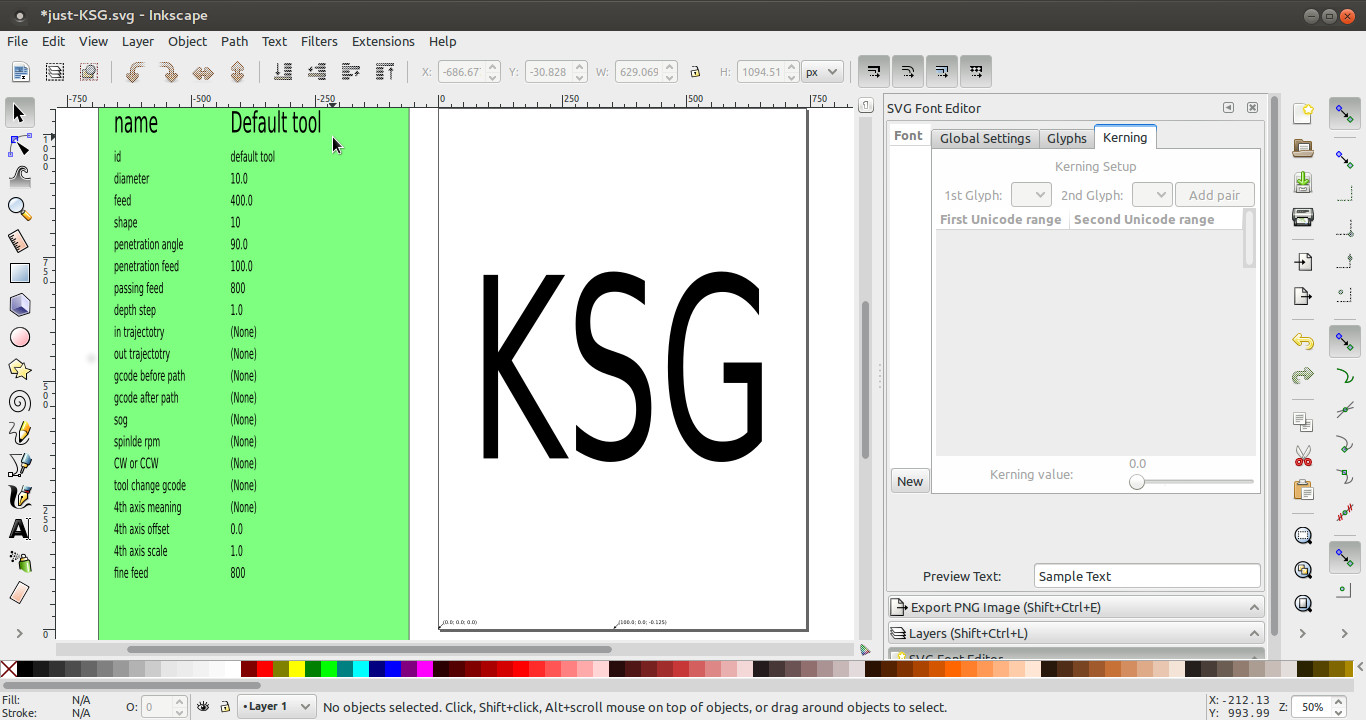
\includegraphics[width=1.3\textwidth]{./07-images/img-Ch4App/Inkscape-Display-of-2D-KSG.jpg}}
		\caption{App4-Inkscape display of 2D KSG jpg file.}
		\label{fig:App4-Inkscape-Display-of-2D-KSG.jpg}
	\end{center}
\end{figure}

% ========================================================
\pagebreak
\textbf{Display Text for 2D KSG model SVG/XML (Clipped text from 671 lines total)}

% ==========================================================
\lstset{basicstyle=\footnotesize, numberstyle=\tiny\color{blue}, frame=single, numbers=left, firstnumber=1, stepnumber=1, numbersep=1pt, xleftmargin=2.0em, framexleftmargin=1.5em, xrightmargin=0.0em, breaklines=true, breakatwhitespace=false, breakindent=5pt, prebreak=\space, postbreak=\space }
% ==========================================================

\begin{lstlisting}[caption={App4-Display Text for 2D KSG model SVG/XML}, label=App4-Display Text for 2D KSG model SVG/XML]
<?xml version="1.0" encoding="UTF-8" standalone="no"?>
<!-- Created with Inkscape (http://www.inkscape.org/) -->

<svg
xmlns:dc="http://purl.org/dc/elements/1.1/"
xmlns:cc="http://creativecommons.org/ns#"
xmlns:rdf="http://www.w3.org/1999/02/22-rdf-syntax-ns#"
xmlns:svg="http://www.w3.org/2000/svg"
xmlns="http://www.w3.org/2000/svg"
xmlns:sodipodi="http://sodipodi.sourceforge.net/DTD/sodipodi-0.dtd"
xmlns:inkscape="http://www.inkscape.org/namespaces/inkscape"
	width="210mm"
	height="297mm"
	viewBox="0 0 744.09448819 1052.3622047"
	id="svg4749"
	version="1.1"
	inkscape:version="0.91 r13725"
	sodipodi:docname="just-KSG.svg">
	<sodipodi:namedview
	id="base"
	pagecolor="#ffffff"
	bordercolor="#666666"
	borderopacity="1.0"
	inkscape:pageopacity="0.0"
	inkscape:pageshadow="2"
	inkscape:zoom="0.35"
	inkscape:cx="375"
	inkscape:cy="520"
	inkscape:document-units="px"
	inkscape:current-layer="layer1"
	showgrid="false"
	inkscape:window-width="1366"
	inkscape:window-height="689"
	inkscape:window-x="0"
	inkscape:window-y="24"
	inkscape:window-maximized="1" />
	<defs
	id="defs4751" />
	<metadata
	id="metadata4754">
	<rdf:RDF>
	<cc:Work
	rdf:about="">
	<dc:format>image/svg+xml</dc:format>
	<dc:type
	rdf:resource="http://purl.org/dc/dcmitype/StillImage" />
	<dc:title></dc:title>
	</cc:Work>
	</rdf:RDF>
	</metadata>
	<g
	id="layer1"
	inkscape:groupmode="layer"
	inkscape:label="Layer 1">
	<text
	transform="scale(0.76565133,1.3060775)"
	sodipodi:linespacing="125%"
	id="text4757"
	y="554.98346"
	x="81.874046"
	style="font-style:normal;font-weight:normal;font-size:389.44628906px;line-height:125%;font-family:sans-serif;letter-spacing:0px;word-spacing:0px;fill:#000000;fill-opacity:1;stroke:none;stroke-width:1px;stroke-linecap:butt;stroke-linejoin:miter;stroke-opacity:1"
	xml:space="preserve"><tspan
	y="554.98346"
	x="81.874046"
	id="tspan4759"
	sodipodi:role="line">KSG</tspan></text>
	<g
	id="g4787"
	gcodetools="Gcodetools orientation group">
	<g
	id="g4789"
	gcodetools="Gcodetools orientation point (2 points)">
	<path
	id="path4791"
	style="stroke:none;fill:#000000;"
	gcodetools="Gcodetools orientation point arrow"
	d="m 0.0,1052.36220472 2.9375,-6.343750000001 0.8125,1.90625 6.843748640396,-6.84374864039 0,0 0.6875,0.6875 -6.84375,6.84375 1.90625,0.812500000001 z z" />
	<text
	id="text4793"
	xml:space="preserve"
	y="1042.36220472"
	x="10.0"
	style="font-family:DejaVu Sans;font-style:normal;font-variant:normal;font-weight:normal;font-stretch:normal;font-family:DejaVu Sans;fill:#000000;fill-opacity:1;stroke:none;font-size:10.000000px;"
	gcodetools="Gcodetools orientation point text"><tspan
	id="tspan4795"
	sodipodi:role="line"
	y="1042.36220472"
	x="10.0">(0.0; 0.0; 0.0)</tspan></text>
	</g>

.... BEGIN CLIPPED TEXT
....
.... END CLIPPED TEXT
        x="150"
       style="font-style:normal;font-variant:normal;font-weight:normal;font-stretch:normal;font-size:10px;font-family:'DejaVu Sans';fill:#000000;fill-opacity:1;stroke:none"
       gcodetools="Gcodetools tool definition field value"><tspan
       id="tspan5017"
       sodipodi:role="line"
       y="305"
       x="150">800</tspan></text>
       </g>
       </g>
       </g>
       <g
       id="g5019" />
</svg>
THE END AT LINE 671      
\end{lstlisting}
% ===========================================================


\pagebreak
\clearpage
%===========================================================

% =========================================================
\subsection{App4-Creation of G-Code for 2D Model}\label{sec:App4-Creation of G-Code for 2D Model}
% =========================================================

\begin{enumerate}
	%%\vspace{0.2cm}
	
\item \textbf{CAM software tracing 2D model KSG drawing}

To convert the model into G-Code, some software tool, like CAM, must trace the 2D model drawing (SVG or STL) for lines, curves and surfaces, then capture and save those point traces as numerical data into a file. These points saved into the file are only geometrical points. There are no instruction commands for a CNC machine to follow inside this file.

\item \textbf{CAM software added machining instructions to make G-Code}

The next step for CAM, is to read the numerical data file, determine how a machine should trace the geometrical codes, and add these machine instructions into the data file. Now the file becomes a G-code file. 

This CAM file trace includes not only captures of the points as numerical path data (G series), but also CNC tool movements like speeds (F series) to move along the data points as well as associated CNC tool jumps from point-to-point. In addition, CNC service commands are also added into the G-Code file, like (M series) to start and stop the tool, to start and stop lubrication fluids, to pause and change tool cutters, and so on. 
 
Typically, the (G00, G01. G02 and G03) are the primary movement commands generated in conversion from models to G-Code files.

Note that, a CAD model drawing file only contains path data and geometric elements. It does not contain CNC machine movements and other machine service instructions.
 
% \vspace{0.2cm}
\item \textbf{Intensive CAM software computations to produce G-Code}

% \vspace{0.2cm}
Just consider a simple 2D model of the letters "KSG" as we have shown in the previous section. For that, the CAM engine must process about 700 lines of SVG text codes to produce the G-Code file. Imagine, for very large and complex 2D and 3D model drawings, for example, large SVG, STL files. The conversion of these model drawings to G-Code can be very time consuming, like hours to complete. And the resulting G-Code files can run into thousands of G-Code command lines. 
vspace{0.2cm}

A single command instruction in G-Code file is usually written as a one line entry. This varies depending on the G-Codes standard in practice. Because of efficient curve interpolation, NURBS entries in G-Code like G06 series, make the overall G-Code file size smaller. However, NURBS G-Code entries are generally more complicated to interpret and execute by the CNC Interpreter and CNC Interpolator software, compared to common G01, G02 and G03 codes. High end FANUC CNC machines implement NURBS interpolation and they have their own software (proprietary) to accomplish that.
\vspace{0.2cm}

In our illustration example, the KSG 2D drawing is simple, and only contains linear and arc elements with an SVG file consisting of about 700 lines. This number varies depending on software graphic applications and their vector format. For this drawing, we generated a G-Code file in RS274D NGC format with just 200 lines. This file does not contain NURBS G-Codes.
\vspace{0.2cm}

An excerpt showing typical motion commands like G00, G01, G02 and G03 in G-Code for the KSG 2D model can be seen following that at Listing \ref{App4-Display excerpt listing for 2D KSG G-Code} .

The full textual contents of the G-Code generated file for our KSG 2D model drawing can be seen in the next section at Listing \ref{App4-Display full listing for 2D KSG G-Code} . 

\end{enumerate}

\textbf{Display excerpt listing for 2D KSG G-Code}
\vspace{0.3cm}

Notice that from lines no. 27 until line no. 51 in this excerpt, we can see typical motion commands like G00, G01, G02 and G03 in G-Code. 

% ==========================================================
\lstset{basicstyle=\footnotesize, numberstyle=\tiny\color{blue}, frame=single, numbers=left, firstnumber=1, stepnumber=1, numbersep=1pt, xleftmargin=2.0em, framexleftmargin=1.5em, xrightmargin=0.0em, breaklines=true, breakatwhitespace=false, breakindent=5pt, prebreak=\space, postbreak=\space }
% ==========================================================

\begin{lstlisting}[caption={App4-Display excerpt listing for 2D KSG G-Code}, label=App4-Display excerpt listing for 2D KSG G-Code]
%
(Header)
(Generated by gcodetools from Inkscape.)
(Using default header. To add your own header create file "header" in the output dir.)
M3
(Header end.)
G21 (All units in mm)
#8  = 0 (Z axis offset)
#6  = 0 (X axis offset)
#7  = 0 (Y axis offset)
#10 = 1 (XY Scale factor)
#11 = 1 (Z Scale factor)
#21 = 400.000000 (Feed definition)
#20 = 100.000000 (Feed definition)

(Start cutting path id: path5167)
(Change tool to Default tool)

.... CLIPPED SECTION ----

(Start cutting path id: path5165)
(Change tool to Default tool)

G00 Z[5.000000*#11+#8]
G00 X[117.952117*#10+#6] Y[193.645846*#10+#7]

G01 Z[1.000000*#11+#8] F [#20](Penetrate)
G01 X[117.952117*#10+#6] Y[179.837424*#10+#7] Z[1.000000*#11+#8] F [#21]
G03 X[113.046989*#10+#6] Y[183.402174*#10+#7] Z[1.000000*#11+#8] I[-34.318323*#10] J[-42.065200*#10]
G03 X[109.035511*#10+#6] Y[185.585093*#10+#7] Z[1.000000*#11+#8] I[-16.685118*#10] J[-25.884338*#10]
G03 X[104.749703*#10+#6] Y[187.038280*#10+#7] Z[1.000000*#11+#8] I[-9.591941*#10] J[-21.242475*#10]
G03 X[100.940711*#10+#6] Y[187.477618*#10+#7] Z[1.000000*#11+#8] I[-3.808992*#10] J[-16.292016*#10]
G03 X[94.758678*#10+#6] Y[186.209903*#10+#7] Z[1.000000*#11+#8] I[-0.000000*#10] J[-15.707261*#10]
G03 X[90.462671*#10+#6] Y[182.991632*#10+#7] Z[1.000000*#11+#8] I[4.472674*#10] J[-10.446948*#10]
G03 X[87.912396*#10+#6] Y[178.111685*#10+#7] Z[1.000000*#11+#8] I[10.615970*#10] J[-8.654302*#10]
G03 X[86.805629*#10+#6] Y[170.234616*#10+#7] Z[1.000000*#11+#8] I[27.477917*#10] J[-7.877068*#10]
G03 X[87.568633*#10+#6] Y[163.529681*#10+#7] Z[1.000000*#11+#8] I[29.841487*#10] J[0.000000*#10]
G03 X[89.229960*#10+#6] Y[159.720590*#10+#7] Z[1.000000*#11+#8] I[11.027232*#10] J[2.542666*#10]
G03 X[92.213942*#10+#6] Y[156.922563*#10+#7] Z[1.000000*#11+#8] I[8.237512*#10] J[5.794811*#10]
G03 X[98.516380*#10+#6] Y[154.043014*#10+#7] Z[1.000000*#11+#8] I[15.074024*#10] J[24.655545*#10]
G01 X[103.529404*#10+#6] Y[152.290678*#10+#7] Z[1.000000*#11+#8]
G02 X[111.731935*#10+#6] Y[147.939660*#10+#7] Z[1.000000*#11+#8] I[-8.284484*#10] J[-25.525105*#10]
G02 X[117.212491*#10+#6] Y[141.636464*#10+#7] Z[1.000000*#11+#8] I[-13.341928*#10] J[-17.134888*#10]
G02 X[120.313088*#10+#6] Y[133.703323*#10+#7] Z[1.000000*#11+#8] I[-23.402927*#10] J[-13.719316*#10]
G02 X[121.650249*#10+#6] Y[121.309349*#10+#7] Z[1.000000*#11+#8] I[-56.770488*#10] J[-12.393974*#10]
G02 X[119.784929*#10+#6] Y[106.730189*#10+#7] Z[1.000000*#11+#8] I[-57.907303*#10] J[-0.000000*#10]
G02 X[115.651058*#10+#6] Y[98.248584*#10+#7] Z[1.000000*#11+#8] I[-23.094899*#10] J[6.008071*#10]
G02 X[108.584210*#10+#6] Y[92.631505*#10+#7] Z[1.000000*#11+#8] I[-14.532534*#10] J[11.029440*#10]
G02 X[98.146568*#10+#6] Y[90.398113*#10+#7] Z[1.000000*#11+#8] I[-10.437642*#10] J[23.273202*#10]
G02 X[93.854953*#10+#6] Y[90.783690*#10+#7] Z[1.000000*#11+#8] I[-0.000000*#10] J[24.076414*#10]
G02 X[88.860148*#10+#6] Y[92.080356*#10+#7] Z[1.000000*#11+#8] I[6.155305*#10] J[33.978893*#10]

--- CLIPPED SECTION ----

(Footer)
M5
G00 X0.0000 Y0.0000
M2
(Using default footer. To add your own footer create file "footer" in the output dir.)
(end)
%
\end{lstlisting}

% ==========================================================
\pagebreak
\textbf{Display full listing for 2D KSG G-Code}
\vspace{0.3cm}

% ==========================================================
\lstset{basicstyle=\footnotesize, numberstyle=\tiny\color{blue}, frame=single, numbers=left, firstnumber=1, stepnumber=1, numbersep=1pt, xleftmargin=2.0em, framexleftmargin=1.5em, xrightmargin=0.0em, breaklines=true, breakatwhitespace=false, breakindent=5pt, prebreak=\space, postbreak=\space }
% ==========================================================

\begin{lstlisting}[caption={App4-Display full listing for 2D KSG G-Code}, label=App4-Display full listing for 2D KSG G-Code]
%
(Header)
(Generated by gcodetools from Inkscape.)
(Using default header. To add your own header create file "header" in the output dir.)
M3
(Header end.)
G21 (All units in mm)
#8  = 0 (Z axis offset)
#6  = 0 (X axis offset)
#7  = 0 (Y axis offset)
#10 = 1 (XY Scale factor)
#11 = 1 (Z Scale factor)
#21 = 400.000000 (Feed definition)
#20 = 100.000000 (Feed definition)

(Start cutting path id: path5167)
(Change tool to Default tool)

G00 Z[5.000000*#11+#8]
G00 X[176.423691*#10+#6] Y[107.360743*#10+#7]

G01 Z[1.000000*#11+#8] F [#20](Penetrate)
G01 X[176.423691*#10+#6] Y[135.468236*#10+#7] Z[1.000000*#11+#8] F [#21]
G01 X[162.863873*#10+#6] Y[135.468236*#10+#7] Z[1.000000*#11+#8]
G01 X[162.863873*#10+#6] Y[147.103758*#10+#7] Z[1.000000*#11+#8]
G01 X[184.641760*#10+#6] Y[147.103758*#10+#7] Z[1.000000*#11+#8]
G01 X[184.641760*#10+#6] Y[102.173824*#10+#7] Z[1.000000*#11+#8]
G02 X[179.391923*#10+#6] Y[96.903039*#10+#7] Z[1.000000*#11+#8] I[-30.942596*#10] J[25.569747*#10]
G02 X[174.040450*#10+#6] Y[93.342040*#10+#7] Z[1.000000*#11+#8] I[-19.182522*#10] J[23.025911*#10]
G02 X[168.066958*#10+#6] Y[91.148675*#10+#7] Z[1.000000*#11+#8] I[-12.219785*#10] J[24.048923*#10]
G02 X[161.672253*#10+#6] Y[90.398113*#10+#7] Z[1.000000*#11+#8] I[-6.394705*#10] J[26.865808*#10]
G02 X[149.370262*#10+#6] Y[93.974078*#10+#7] Z[1.000000*#11+#8] I[-0.000000*#10] J[22.948566*#10]
G02 X[139.154740*#10+#6] Y[104.697188*#10+#7] Z[1.000000*#11+#8] I[16.440628*#10] J[25.889933*#10]
G02 X[133.559873*#10+#6] Y[119.722073*#10+#7] Z[1.000000*#11+#8] I[44.792682*#10] J[25.233731*#10]
G02 X[131.059941*#10+#6] Y[144.650484*#10+#7] Z[1.000000*#11+#8] I[123.038549*#10] J[24.928411*#10]
G02 X[133.566449*#10+#6] Y[169.644463*#10+#7] Z[1.000000*#11+#8] I[125.868687*#10] J[0.000000*#10]
G02 X[139.154740*#10+#6] Y[184.603785*#10+#7] Z[1.000000*#11+#8] I[49.856648*#10] J[-10.101281*#10]
G02 X[149.381921*#10+#6] Y[195.385610*#10+#7] Z[1.000000*#11+#8] I[26.785332*#10] J[-15.165982*#10]
G02 X[161.672253*#10+#6] Y[198.972953*#10+#7] Z[1.000000*#11+#8] I[12.290332*#10] J[-19.259830*#10]
G02 X[167.528571*#10+#6] Y[198.331573*#10+#7] Z[1.000000*#11+#8] I[0.000000*#10] J[-27.057176*#10]
G02 X[173.054281*#10+#6] Y[196.449585*#10+#7] Z[1.000000*#11+#8] I[-5.749598*#10] J[-25.934418*#10]
G02 X[178.118029*#10+#6] Y[193.430835*#10+#7] Z[1.000000*#11+#8] I[-12.194513*#10] J[-26.211890*#10]
G02 X[183.039237*#10+#6] Y[189.019673*#10+#7] Z[1.000000*#11+#8] I[-21.688851*#10] J[-29.147349*#10]
G01 X[183.039237*#10+#6] Y[173.949571*#10+#7] Z[1.000000*#11+#8]
G03 X[177.959907*#10+#6] Y[180.117456*#10+#7] Z[1.000000*#11+#8] I[-39.092615*#10] J[-27.017866*#10]
G03 X[173.259733*#10+#6] Y[183.972941*#10+#7] Z[1.000000*#11+#8] I[-19.689245*#10] J[-19.210212*#10]
G03 X[167.837734*#10+#6] Y[186.512086*#10+#7] Z[1.000000*#11+#8] I[-11.832629*#10] J[-18.208427*#10]
G03 X[162.370790*#10+#6] Y[187.337430*#10+#7] Z[1.000000*#11+#8] I[-5.466944*#10] J[-17.693398*#10]
G03 X[152.786893*#10+#6] Y[184.557277*#10+#7] Z[1.000000*#11+#8] I[0.000000*#10] J[-17.909143*#10]
G03 X[145.441564*#10+#6] Y[176.613122*#10+#7] Z[1.000000*#11+#8] I[11.266522*#10] J[-17.785156*#10]
G03 X[141.629050*#10+#6] Y[165.440943*#10+#7] Z[1.000000*#11+#8] I[33.955998*#10] J[-17.824110*#10]
G03 X[139.812185*#10+#6] Y[144.650484*#10+#7] Z[1.000000*#11+#8] I[118.044621*#10] J[-20.790459*#10]
G03 X[141.626890*#10+#6] Y[123.929590*#10+#7] Z[1.000000*#11+#8] I[119.206343*#10] J[-0.000000*#10]
G03 X[145.441564*#10+#6] Y[112.757940*#10+#7] Z[1.000000*#11+#8] I[37.812227*#10] J[6.674267*#10]
G03 X[152.786892*#10+#6] Y[104.813789*#10+#7] Z[1.000000*#11+#8] I[18.611844*#10] J[9.841002*#10]
G03 X[162.370790*#10+#6] Y[102.033636*#10+#7] Z[1.000000*#11+#8] I[9.583897*#10] J[15.128996*#10]
G03 X[166.706157*#10+#6] Y[102.379890*#10+#7] Z[1.000000*#11+#8] I[0.000000*#10] J[27.314245*#10]
G03 X[170.219047*#10+#6] Y[103.295320*#10+#7] Z[1.000000*#11+#8] I[-3.020477*#10] J[18.788763*#10]
G03 X[173.456867*#10+#6] Y[104.956924*#10+#7] Z[1.000000*#11+#8] I[-6.197101*#10] J[16.061169*#10]
G03 X[176.423691*#10+#6] Y[107.360743*#10+#7] Z[1.000000*#11+#8] I[-10.386640*#10] J[15.852077*#10]
G01 X[176.423691*#10+#6] Y[107.360743*#10+#7] Z[1.000000*#11+#8]
G00 Z[5.000000*#11+#8]

(End cutting path id: path5167)

(Start cutting path id: path5165)
(Change tool to Default tool)

G00 Z[5.000000*#11+#8]
G00 X[117.952117*#10+#6] Y[193.645846*#10+#7]

G01 Z[1.000000*#11+#8] F [#20](Penetrate)
G01 X[117.952117*#10+#6] Y[179.837424*#10+#7] Z[1.000000*#11+#8] F [#21]
G03 X[113.046989*#10+#6] Y[183.402174*#10+#7] Z[1.000000*#11+#8] I[-34.318323*#10] J[-42.065200*#10]
G03 X[109.035511*#10+#6] Y[185.585093*#10+#7] Z[1.000000*#11+#8] I[-16.685118*#10] J[-25.884338*#10]
G03 X[104.749703*#10+#6] Y[187.038280*#10+#7] Z[1.000000*#11+#8] I[-9.591941*#10] J[-21.242475*#10]
G03 X[100.940711*#10+#6] Y[187.477618*#10+#7] Z[1.000000*#11+#8] I[-3.808992*#10] J[-16.292016*#10]
G03 X[94.758678*#10+#6] Y[186.209903*#10+#7] Z[1.000000*#11+#8] I[-0.000000*#10] J[-15.707261*#10]
G03 X[90.462671*#10+#6] Y[182.991632*#10+#7] Z[1.000000*#11+#8] I[4.472674*#10] J[-10.446948*#10]
G03 X[87.912396*#10+#6] Y[178.111685*#10+#7] Z[1.000000*#11+#8] I[10.615970*#10] J[-8.654302*#10]
G03 X[86.805629*#10+#6] Y[170.234616*#10+#7] Z[1.000000*#11+#8] I[27.477917*#10] J[-7.877068*#10]
G03 X[87.568633*#10+#6] Y[163.529681*#10+#7] Z[1.000000*#11+#8] I[29.841487*#10] J[0.000000*#10]
G03 X[89.229960*#10+#6] Y[159.720590*#10+#7] Z[1.000000*#11+#8] I[11.027232*#10] J[2.542666*#10]
G03 X[92.213942*#10+#6] Y[156.922563*#10+#7] Z[1.000000*#11+#8] I[8.237512*#10] J[5.794811*#10]
G03 X[98.516380*#10+#6] Y[154.043014*#10+#7] Z[1.000000*#11+#8] I[15.074024*#10] J[24.655545*#10]
G01 X[103.529404*#10+#6] Y[152.290678*#10+#7] Z[1.000000*#11+#8]
G02 X[111.731935*#10+#6] Y[147.939660*#10+#7] Z[1.000000*#11+#8] I[-8.284484*#10] J[-25.525105*#10]
G02 X[117.212491*#10+#6] Y[141.636464*#10+#7] Z[1.000000*#11+#8] I[-13.341928*#10] J[-17.134888*#10]
G02 X[120.313088*#10+#6] Y[133.703323*#10+#7] Z[1.000000*#11+#8] I[-23.402927*#10] J[-13.719316*#10]
G02 X[121.650249*#10+#6] Y[121.309349*#10+#7] Z[1.000000*#11+#8] I[-56.770488*#10] J[-12.393974*#10]
G02 X[119.784929*#10+#6] Y[106.730189*#10+#7] Z[1.000000*#11+#8] I[-57.907303*#10] J[-0.000000*#10]
G02 X[115.651058*#10+#6] Y[98.248584*#10+#7] Z[1.000000*#11+#8] I[-23.094899*#10] J[6.008071*#10]
G02 X[108.584210*#10+#6] Y[92.631505*#10+#7] Z[1.000000*#11+#8] I[-14.532534*#10] J[11.029440*#10]
G02 X[98.146568*#10+#6] Y[90.398113*#10+#7] Z[1.000000*#11+#8] I[-10.437642*#10] J[23.273202*#10]
G02 X[93.854953*#10+#6] Y[90.783690*#10+#7] Z[1.000000*#11+#8] I[-0.000000*#10] J[24.076414*#10]
G02 X[88.860148*#10+#6] Y[92.080356*#10+#7] Z[1.000000*#11+#8] I[6.155305*#10] J[33.978893*#10]
G02 X[84.109236*#10+#6] Y[94.053384*#10+#7] Z[1.000000*#11+#8] I[13.446482*#10] J[39.084622*#10]
G02 X[78.710831*#10+#6] Y[97.056998*#10+#7] Z[1.000000*#11+#8] I[26.242970*#10] J[53.519667*#10]
G01 X[78.710831*#10+#6] Y[111.636444*#10+#7] Z[1.000000*#11+#8]
G03 X[84.025978*#10+#6] Y[107.168820*#10+#7] Z[1.000000*#11+#8] I[37.287981*#10] J[38.966103*#10]
G03 X[88.613605*#10+#6] Y[104.346723*#10+#7] Z[1.000000*#11+#8] I[19.239604*#10] J[26.136178*#10]
G03 X[93.599617*#10+#6] Y[102.469141*#10+#7] Z[1.000000*#11+#8] I[11.130303*#10] J[21.997980*#10]
G03 X[98.146568*#10+#6] Y[101.893449*#10+#7] Z[1.000000*#11+#8] I[4.546951*#10] J[17.668599*#10]
G03 X[104.614313*#10+#6] Y[103.237701*#10+#7] Z[1.000000*#11+#8] I[-0.000000*#10] J[16.231605*#10]
G03 X[109.117692*#10+#6] Y[106.659805*#10+#7] Z[1.000000*#11+#8] I[-4.741455*#10] J[10.913805*#10]
G03 X[111.808038*#10+#6] Y[111.841476*#10+#7] Z[1.000000*#11+#8] I[-11.297040*#10] J[9.154726*#10]
G03 X[112.980184*#10+#6] Y[120.257946*#10+#7] Z[1.000000*#11+#8] I[-29.630701*#10] J[8.416470*#10]
G03 X[112.127054*#10+#6] Y[127.717636*#10+#7] Z[1.000000*#11+#8] I[-33.039967*#10] J[0.000000*#10]
G03 X[110.186041*#10+#6] Y[132.314028*#10+#7] Z[1.000000*#11+#8] I[-14.213271*#10] J[-3.294098*#10]
G03 X[106.818823*#10+#6] Y[135.882125*#10+#7] Z[1.000000*#11+#8] I[-10.873106*#10] J[-6.888092*#10]
G03 X[101.105073*#10+#6] Y[138.832725*#10+#7] Z[1.000000*#11+#8] I[-12.895623*#10] J[-17.964440*#10]
G01 X[96.050959*#10+#6] Y[140.514968*#10+#7] Z[1.000000*#11+#8]
G02 X[87.715741*#10+#6] Y[144.862945*#10+#7] Z[1.000000*#11+#8] I[9.895237*#10] J[29.132934*#10]
G02 X[82.614413*#10+#6] Y[150.398154*#10+#7] Z[1.000000*#11+#8] I[11.687787*#10] J[15.889965*#10]
G02 X[79.737752*#10+#6] Y[157.488256*#10+#7] Z[1.000000*#11+#8] I[19.564586*#10] J[12.066546*#10]
G02 X[78.464288*#10+#6] Y[169.113120*#10+#7] Z[1.000000*#11+#8] I[52.422259*#10] J[11.624864*#10]
G02 X[80.176218*#10+#6] Y[182.442710*#10+#7] Z[1.000000*#11+#8] I[52.750021*#10] J[0.000000*#10]
G02 X[84.175848*#10+#6] Y[190.982294*#10+#7] Z[1.000000*#11+#8] I[25.128284*#10] J[-6.562740*#10]
G02 X[91.023399*#10+#6] Y[196.835582*#10+#7] Z[1.000000*#11+#8] I[15.406407*#10] J[-11.091406*#10]
G02 X[99.995634*#10+#6] Y[198.972953*#10+#7] Z[1.000000*#11+#8] I[8.972235*#10] J[-17.763096*#10]
G02 X[104.263355*#10+#6] Y[198.651605*#10+#7] Z[1.000000*#11+#8] I[-0.000000*#10] J[-28.499848*#10]
G02 X[108.788968*#10+#6] Y[197.641175*#10+#7] Z[1.000000*#11+#8] I[-5.009916*#10] J[-33.078997*#10]
G02 X[113.155807*#10+#6] Y[196.046682*#10+#7] Z[1.000000*#11+#8] I[-10.854275*#10] J[-36.503587*#10]
G02 X[117.952117*#10+#6] Y[193.645846*#10+#7] Z[1.000000*#11+#8] I[-20.261739*#10] J[-46.469596*#10]
G01 X[117.952117*#10+#6] Y[193.645846*#10+#7] Z[1.000000*#11+#8]
G00 Z[5.000000*#11+#8]

(End cutting path id: path5165)

(Start cutting path id: path5163)
(Change tool to Default tool)

G00 Z[5.000000*#11+#8]
G00 X[25.950818*#10+#6] Y[197.080429*#10+#7]

G01 Z[1.000000*#11+#8] F [#20](Penetrate)
G01 X[34.251068*#10+#6] Y[197.080429*#10+#7] Z[1.000000*#11+#8] F [#21]
G01 X[34.251068*#10+#6] Y[152.851428*#10+#7] Z[1.000000*#11+#8]
G01 X[61.781606*#10+#6] Y[197.080429*#10+#7] Z[1.000000*#11+#8]
G01 X[72.465097*#10+#6] Y[197.080429*#10+#7] Z[1.000000*#11+#8]
G01 X[42.017145*#10+#6] Y[148.295349*#10+#7] Z[1.000000*#11+#8]
G01 X[74.642884*#10+#6] Y[92.430825*#10+#7] Z[1.000000*#11+#8]
G01 X[63.712853*#10+#6] Y[92.430825*#10+#7] Z[1.000000*#11+#8]
G01 X[34.251068*#10+#6] Y[142.828054*#10+#7] Z[1.000000*#11+#8]
G01 X[34.251068*#10+#6] Y[92.430825*#10+#7] Z[1.000000*#11+#8]
G01 X[25.950818*#10+#6] Y[92.430825*#10+#7] Z[1.000000*#11+#8]
G01 X[25.950818*#10+#6] Y[197.080429*#10+#7] Z[1.000000*#11+#8]
G01 X[25.950818*#10+#6] Y[197.080429*#10+#7] Z[1.000000*#11+#8]
G00 Z[5.000000*#11+#8]

(End cutting path id: path5163)

(Footer)
M5
G00 X0.0000 Y0.0000
M2

(Using default footer. To add your own footer create file "footer" in the output dir.)
(end)
%
\end{lstlisting}

%% =========================================================



\pagebreak
\clearpage
%% END LANDSCAPE ENTIRELY
\end{landscape}
\end{flushleft}
%% ========= END Chapter-4 Appendices ===================== %% Related Research Work
	% ==========================================================
\clearpage
\pagebreak
\justifying
\renewcommand{\thesection}{E \arabic{section}}

\titleformat{\section}{\normalfont\LARGE\bfseries\color{black}}{\thesection}{10pt}{\LARGE}
\section{Appendix-E5 Research Implementation Plan}\label{sec:App5-Research-Implementation-Plan}

%============================================================
\subsection{App5-PhD Proposal Document Preparation}
\begin{figure}[htbp]
	\begin{center}
		\frame{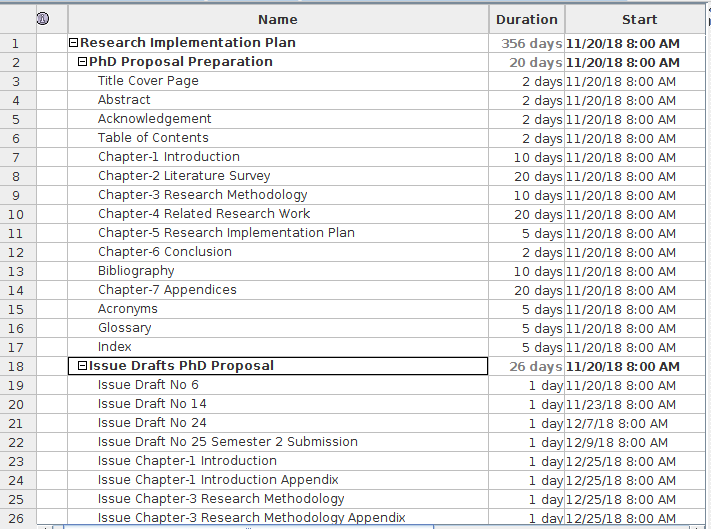
\includegraphics[width=1.00\textwidth]{./07-images/img-Ch5App/01-Research-Implementation-Plan.png}}
		\caption{App5-PhD Proposal Document Preparation}
		\label{fig:App5-01-Research-Implementation-Plan.png}
	\end{center}
\end{figure}

Note that the contents of a proposal document do not include the chapter on implementation design and the chapter on results and discussion, which are both required for a thesis document.

	
\pagebreak	
\subsection{App5-Procurement of Long Lead Items and Project Setup}
\begin{figure}[htbp]
	\begin{center}
		\frame{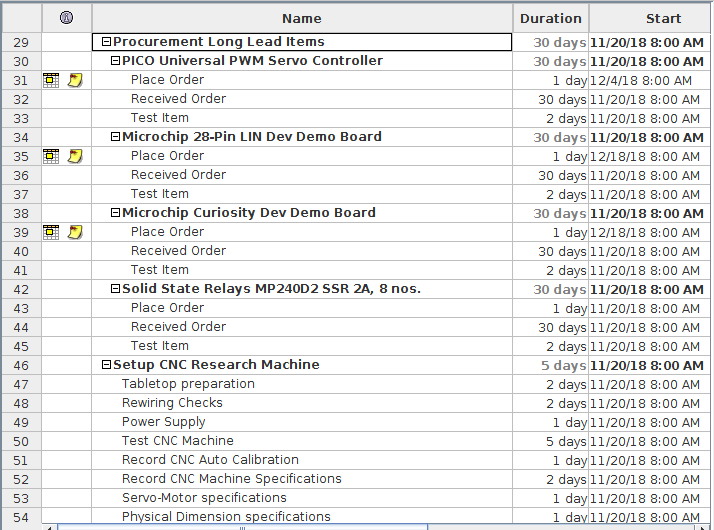
\includegraphics[width=1.00\textwidth]{./07-images/img-Ch5App/02-Research-Implementation-Plan.png}}
		\caption{App5-Procurement of Long Lead Items and Project Setup}
		\label{fig:App5-02-Research-Implementation-Plan.png}
	\end{center}
\end{figure}

The long lead items above are hardware resources that must be procured for the project.

\pagebreak
\subsection{App5-Computer 64bit Resources and Software Installations}
\begin{figure}[htbp]
	\begin{center}
		\frame{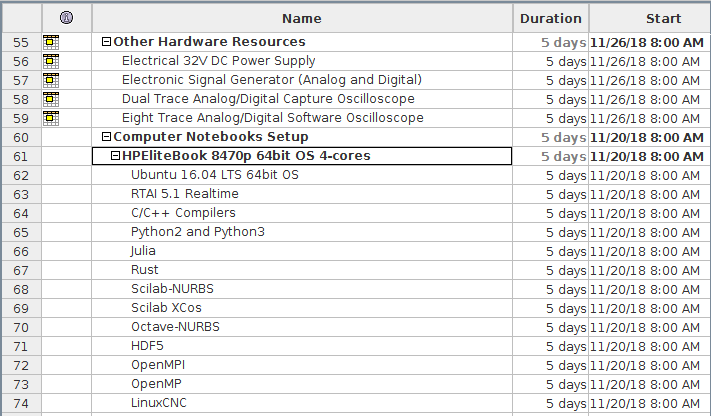
\includegraphics[width=1.00\textwidth]{./07-images/img-Ch5App/03-Research-Implementation-Plan.png}}
		\caption{App5-Computer 64bit Resources and Software Installations}
		\label{fig:App5-03-Research-Implementation-Plan.png}
	\end{center}
\end{figure}

We will be implementing the CNC Control software on both 64bit and 32bit systems. The Linux kernel for the 64bit system is of version 4.X, while that for the 32bit system is of version 3.X. The Realtime RTAI library for the 64bit system is of version 5.1, while that for the 32bit system is version 2.7.  
\vspace{0.5cm}

The above tasks in the figure identify the 64bit hardware resources and their associated software that are required for the project.

\pagebreak
\subsection{App5-Computer 32bit Resources and Software Installations}
\begin{figure}[htbp]
	\begin{center}
		\frame{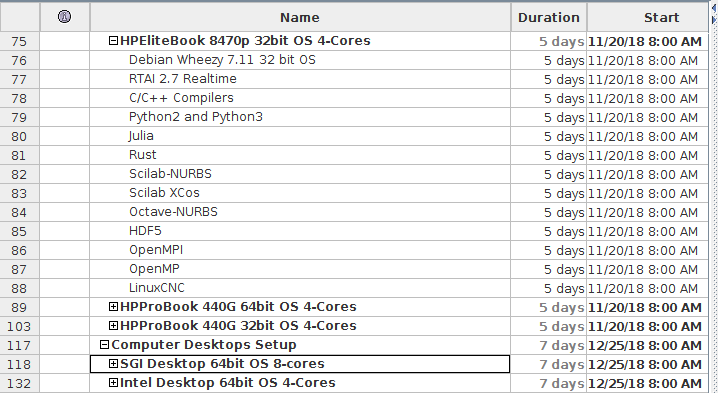
\includegraphics[width=1.00\textwidth]{./07-images/img-Ch5App/04-Research-Implementation-Plan.png}}
		\caption{App5-Computer 32bit Resources and Software Installations}
		\label{fig:App5-04-Research-Implementation-Plan.png}
	\end{center}
\end{figure}

We will be implementing the CNC Control software on four(4) different computer hardware configurations (number of CPU cores, memory speeds, hard disk speeds, etc) for the purposes of performance comparisons. The multi-core feature of the computers is for true parallel computation design. The different computers are as follows:

\begin{enumerate}
	\item Notebook HP EliteBook 8470p, 4-cores, installed with both 64bit and 32bit Linux operating systems.   
	
	\item Notebook HP ProBook 440G, 4-cores, installed with both 64bit and 32bit Linux operating systems.
	
	\item Desktop SGI, 8-cores, installed with only 64bit Linux operating system. Does not accept 32bit OS.
	
	\item Desktop Intel, 4-cores, installed with both 64bit and 32bit Linux operating systems.
\end{enumerate}

The above tasks in the figure identify the 32bit hardware resources and their associated software that are required for the project.

\pagebreak
\subsection{App5-UseCase Design and Software Architecture Design}\label{sec:App5-UseCase Design}
\begin{figure}[htbp]
	\begin{center}
		\frame{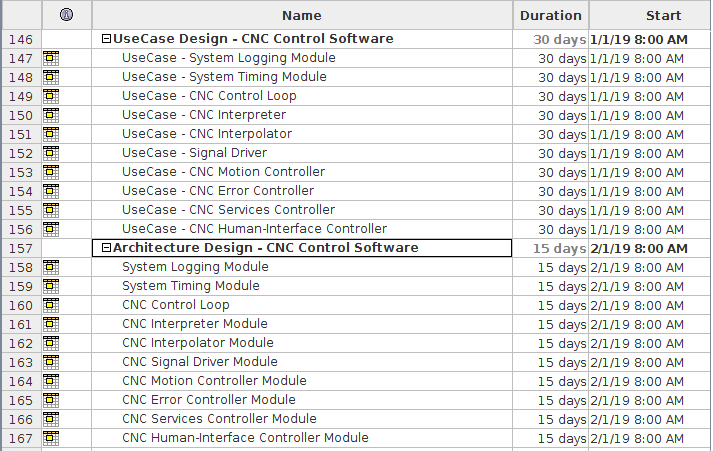
\includegraphics[width=1.00\textwidth]{./07-images/img-Ch5App/05-Research-Implementation-Plan.png}}
		\caption{App5-UseCase Design and Software Architecture Design}
		\label{fig:App5-05-Research-Implementation-Plan.png}
	\end{center}
\end{figure}


\pagebreak	
\subsection{App5-Process and Data Flow Design for the Control Loop}\label{sec:App5-Process-Flow Design}
\begin{figure}[htbp]
	\begin{center}
		\frame{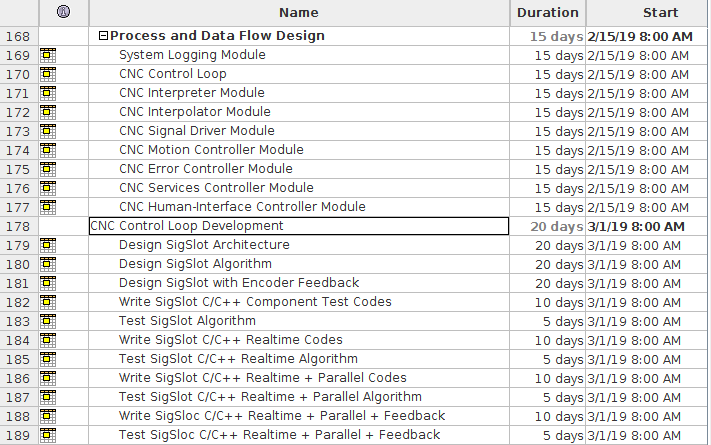
\includegraphics[width=1.00\textwidth]{./07-images/img-Ch5App/06-Research-Implementation-Plan.png}}
		\caption{App5-Process and Data Flow Design for the Control Loop}
		\label{fig:App5-06-Research-Implementation-Plan.png}
	\end{center}
\end{figure}

\pagebreak
\subsection{App5-Test-Case Based Design in Software Construction}
\begin{figure}[htbp]
	\begin{center}
		\frame{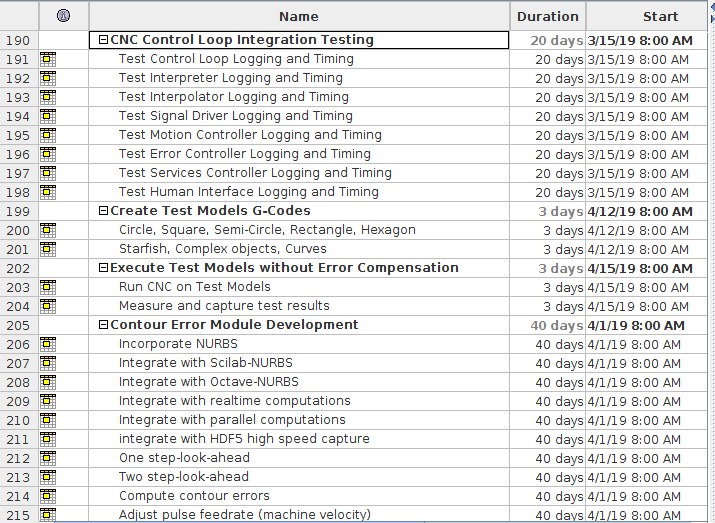
\includegraphics[width=1.00\textwidth]{./07-images/img-Ch5App/07-Research-Implementation-Plan.png}}
		\caption{App5-Test-Case Based Design in Software Construction}
		\label{fig:App5-07-Research-Implementation-Plan.png}
	\end{center}
\end{figure}

\pagebreak
\subsection{App5-Completion Testing, Publication Plan and Project Closing}
\begin{figure}[htbp]
	\begin{center}
		\frame{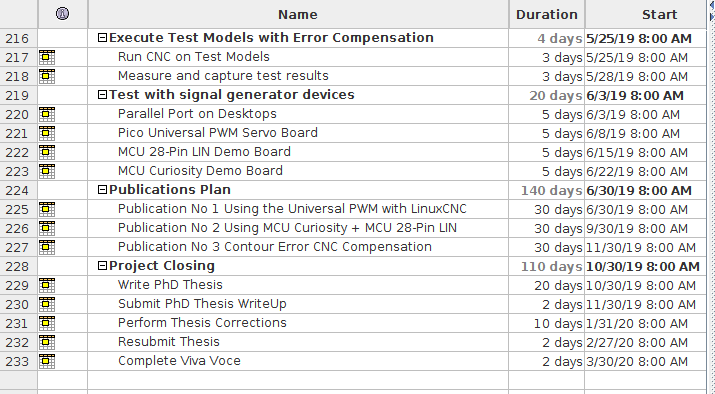
\includegraphics[width=1.00\textwidth]{./07-images/img-Ch5App/08-Research-Implementation-Plan.png}}
		\caption{App5-Completion Testing, Publication Plan and Project Closing}
		\label{fig:App5-08-Research-Implementation-Plan.png}
	\end{center}
\end{figure}

% ==========================================================
% ==========================================================
\clearpage
\begin{landscape}
\subsection{App5-Computer Notebook Specifications}
	
\begin{table}[ht]
\begin{center}
\caption{App5-Computer Notebook Specifications}		
\label{table:App5-Computer Notebook Specifications}	
	
\begin{tabular}{ |p{0.5cm}|p{5.0cm}|p{9.0cm}|p{9.0cm}|}
	\rowcolor{gray!10}			
	\hline \multicolumn{4}{|c|}{\textbf{Computer Notebook Specifications}} \\ [1.0ex]
	\rowcolor{gray!10}
	\hline \textbf{No} & \textbf{Specifications}    & \textbf{Hewlett Packard EliteBook 8470p} & \textbf{Hewlett Packard ProBook 440G}\\ 

	\hline 1 & Name of Student    & Wan Ruslan bin W Yusoff & hello\\ 
	\hline 2 & Student ID         &  aaa & Hello\\ 
	\hline 3 & National Reg. ID   & bbb  & Hello\\ 
	\hline 4 & Faculty            & ccc  & Hello\\ 

	\hline
\end{tabular}
\end{center}
\end{table}  
	
	
\end{landscape}
% ==========================================================
% ==========================================================
\clearpage
\begin{landscape}
\subsection{App5-Computer Desktop Specifications}
	
	\begin{table}[ht]
		\begin{center}
			\caption{App5-Computer Desktop Specifications}		
			\label{table:App5-Computer Desktop Specifications}	
			
			\begin{tabular}{ |p{0.5cm}|p{5.0cm}|p{9.0cm}|p{9.0cm}|}
				\rowcolor{gray!10}			
				\hline \multicolumn{4}{|c|}{\textbf{Computer Desktop Specifications}} \\ [1.0ex]
				\rowcolor{gray!10}
				\hline \textbf{No} & \textbf{Specifications}  & \textbf{WRY Intel Desktop} & \textbf{WRY SGI Desktop}\\ 
				
				\hline 1 & Name of Student    & Wan Ruslan bin W Yusoff & hello\\ 
				\hline 2 & Student ID         &  aaa & Hello\\ 
				\hline 3 & National Reg. ID   & bbb  & Hello\\ 
				\hline 4 & Faculty            & ccc  & Hello\\ 
				
				\hline
			\end{tabular}
		\end{center}
	\end{table}  
	
	
\end{landscape}
% ==========================================================
% ==========================================================
\clearpage
\begin{landscape}
\subsection{App5-Pulse Generator Interface Boards}
	
	\begin{table}[ht]
		\begin{center}
			\caption{App5-Pulse Generator Interface Boards}		
			\label{table:App5-Pulse Generator Interface Boards}	
			
			\begin{tabular}{ |p{0.5cm}|p{5.0cm}|p{6.0cm}|p{6.0cm}|p{6.0cm}|}
				\rowcolor{gray!10}			
				\hline \multicolumn{5}{|c|}{\textbf{Pulse Generator Interface Boards}} \\ [1.0ex]
				\rowcolor{gray!10}
				\hline \textbf{No} & \textbf{Specifications}    & \textbf{Pico Universal PWM Servo Controller Board} & \textbf{MCU Microchip 28-Pin LIN Development Board} & \textbf{MCU Microchip Curiosity Development Board}\\ 
				
				\hline 1 & Name of Student    & Wan Ruslan bin W Yusoff & hello & Hello\\ 
				\hline 2 & Student ID         &  aaa & Hello & hello\\ 
				\hline 3 & National Reg. ID   & bbb  & Hello & Hello \\ 
				\hline 4 & Faculty            & ccc  & Hello & Hello\\ 
				
				\hline
			\end{tabular}
		\end{center}
	\end{table}  
	
	
\end{landscape}
% ==========================================================
% ==========================================================
\clearpage
\begin{landscape}
\subsection{App5-Software Programming Language Features}

	
	\begin{table}[ht]
		\begin{center}
			\caption{App5-Software Programming Language Features}		
			\label{table:App5-Software Programming Language Features}	
			
			\begin{tabular}{ |p{0.5cm}|p{5.0cm}|p{9.0cm}|p{9.0cm}|}
				\rowcolor{gray!10}			
				\hline \multicolumn{4}{|c|}{\textbf{Software Programming Language Features}} \\ [1.0ex]
				\rowcolor{gray!10}
				\hline \textbf{No} & \textbf{Specifications}    & \textbf{Hewlett Packard EliteBook 8470p} & \textbf{Hewlett Packard ProBook 440G}\\ 
				
				\hline 1 & Name of Student    & Wan Ruslan bin W Yusoff & hello\\ 
				\hline 2 & Student ID         &  aaa & Hello\\ 
				\hline 3 & National Reg. ID   & bbb  & Hello\\ 
				\hline 4 & Faculty            & ccc  & Hello\\ 
				
				\hline
			\end{tabular}
		\end{center}
	\end{table}  
	
	
\end{landscape}
% ==========================================================
% ==========================================================
\clearpage
\begin{landscape}
\subsection{App5-Software Programming Paradigms}
	
	\begin{table}[ht]
		\begin{center}
			\caption{App5-Software Programming Paradigms}		
			\label{table:App5-Software Programming Paradigms}	
			
			\begin{tabular}{ |p{0.5cm}|p{5.0cm}|p{9.0cm}|p{9.0cm}|}
				\rowcolor{gray!10}			
				\hline \multicolumn{4}{|c|}{\textbf{Software Programming Paradigms}} \\ [1.0ex]
				\rowcolor{gray!10}
				\hline \textbf{No} & \textbf{Specifications}    & \textbf{Hewlett Packard EliteBook 8470p} & \textbf{Hewlett Packard ProBook 440G}\\ 
				
				\hline 1 & Name of Student    & Wan Ruslan bin W Yusoff & hello\\ 
				\hline 2 & Student ID         &  aaa & Hello\\ 
				\hline 3 & National Reg. ID   & bbb  & Hello\\ 
				\hline 4 & Faculty            & ccc  & Hello\\ 
				
				\hline
			\end{tabular}
		\end{center}
	\end{table}  
	
\end{landscape}	
% ==========================================================
% ==========================================================
\clearpage
\begin{landscape}
	\subsection{App5-Scilab NURBS versus Octave NURBS packages}
	
	\begin{table}[ht]
		\begin{center}
			\caption{App5-Scilab NURBS versus Octave NURBS packages}		
			\label{tabl2:App5-Scilab NURBS versus Octave NURBS packages}	
			
			\begin{tabular}{ |p{0.5cm}|p{5.0cm}|p{9.0cm}|p{9.0cm}|}
				\rowcolor{gray!10}			
				\hline \multicolumn{4}{|c|}{\textbf{Scilab NURBS versus Octave NURBS packages}} \\ [1.0ex]
				\rowcolor{gray!10}
				\hline \textbf{No} & \textbf{Specifications}    & \textbf{Hewlett Packard EliteBook 8470p} & \textbf{Hewlett Packard ProBook 440G}\\ 
				
				\hline 1 & Name of Student    & Wan Ruslan bin W Yusoff & hello\\ 
				\hline 2 & Student ID         &  aaa & Hello\\ 
				\hline 3 & National Reg. ID   & bbb  & Hello\\ 
				\hline 4 & Faculty            & ccc  & Hello\\ 
				
				\hline
			\end{tabular}
		\end{center}
	\end{table}  
	
\end{landscape}
% ==========================================================
% ==========================================================
\clearpage
\begin{landscape}
	\subsection{App5-Python versus Julia programming languages}
	
	\begin{table}[ht]
		\begin{center}
			\caption{App5-Python versus Julia programming languages}		
			\label{tabl2:App5-Python versus Julia programming languages}	
			
			\begin{tabular}{ |p{0.5cm}|p{5.0cm}|p{9.0cm}|p{9.0cm}|}
				\rowcolor{gray!10}			
				\hline \multicolumn{4}{|c|}{\textbf{Python versus Julia programming languages}} \\ [1.0ex]
				\rowcolor{gray!10}
				\hline \textbf{No} & \textbf{Specifications}    & \textbf{Hewlett Packard EliteBook 8470p} & \textbf{Hewlett Packard ProBook 440G}\\ 
				
				\hline 1 & Name of Student    & Wan Ruslan bin W Yusoff & hello\\ 
				\hline 2 & Student ID         &  aaa & Hello\\ 
				\hline 3 & National Reg. ID   & bbb  & Hello\\ 
				\hline 4 & Faculty            & ccc  & Hello\\ 
				
				\hline
			\end{tabular}
		\end{center}
	\end{table}  
	
\end{landscape}
% ==========================================================
% ==========================================================
\clearpage
\begin{landscape}
	\subsection{App5-C/C++ versus Rust system programming languages}
	
	\begin{table}[ht]
		\begin{center}
			\caption{App5-C/C++ versus Rust system programming languages}		
			\label{tabl2:App5-C/C++ versus Rust system programming languages}	
			
			\begin{tabular}{ |p{0.5cm}|p{5.0cm}|p{9.0cm}|p{9.0cm}|}
				\rowcolor{gray!10}			
				\hline \multicolumn{4}{|c|}{\textbf{C/C++ versus Rust system programming languages}} \\ [1.0ex]
				\rowcolor{gray!10}
				\hline \textbf{No} & \textbf{Specifications}    & \textbf{Hewlett Packard EliteBook 8470p} & \textbf{Hewlett Packard ProBook 440G}\\ 
				
				\hline 1 & Name of Student    & Wan Ruslan bin W Yusoff & hello\\ 
				\hline 2 & Student ID         &  aaa & Hello\\ 
				\hline 3 & National Reg. ID   & bbb  & Hello\\ 
				\hline 4 & Faculty            & ccc  & Hello\\ 
				
				\hline
			\end{tabular}
		\end{center}
	\end{table}  
	
\end{landscape}
% ==========================================================
% ==========================================================
 %% Research Implementation Plan
	%\input{Appendix-Chap-6} %% Conclusion ==> NOT APPLICABLE
	\input{Chapter-10-Index}  %% ADDED TEMPORARILY
	...
	...
\end{lstlisting}
\end{tcolorbox}
